%%%%%%%%%%%%%%%%%%%%%%% file template.tex %%%%%%%%%%%%%%%%%%%%%%%%%
%
% This is a general template file for the LaTeX package SVJour3
% for Springer journals.          Springer Heidelberg 2010/09/16
%
% Copy it to a new file with a new name and use it as the basis
% for your article. Delete % signs as needed.
%
% This template includes a few options for different layouts and
% content for various journals. Please consult a previous issue of
% your journal as needed.
%
%%%%%%%%%%%%%%%%%%%%%%%%%%%%%%%%%%%%%%%%%%%%%%%%%%%%%%%%%%%%%%%%%%%
%
% First comes an example EPS file -- just ignore it and
% proceed on the \documentclass line
% your LaTeX will extract the file if required
\begin{filecontents*}{example.eps}
%!PS-Adobe-3.0 EPSF-3.0
%%BoundingBox: 19 19 221 221
%%CreationDate: Mon Sep 29 1997
%%Creator: programmed by hand (JK)
%%EndComments
gsave
newpath
  20 20 moveto
  20 220 lineto
  220 220 lineto
  220 20 lineto
closepath
2 setlinewidth
gsave
  .4 setgray fill
grestore
stroke
grestore
\end{filecontents*}
%
\RequirePackage{fix-cm}
%
%\documentclass{svjour3}                     % onecolumn (standard format)
%\documentclass[smallcondensed]{svjour3}     % onecolumn (ditto)
%\documentclass[smallextended]{svjour3}       % onecolumn (second format)
\documentclass[twocolumn]{svjour3}          % twocolumn
%
\smartqed  % flush right qed marks, e.g. at end of proof
%
\usepackage{graphicx}
\usepackage{times}
\usepackage{epsfig}
\usepackage{epstopdf}
\usepackage{amsmath}
\usepackage{amssymb}
\usepackage{subfigure}
\usepackage{caption}
\usepackage{tabularx}
\usepackage[table]{xcolor}
% Strike through text
 \usepackage[normalem]{ulem}
\usepackage{algorithm}
\usepackage[noend]{algpseudocode}
%
% \usepackage{mathptmx}      % use Times fonts if available on your TeX system
%
% insert here the call for the packages your document requires
%\usepackage{latexsym}
% etc.
%
% Somethong for pseudo algorithms
\makeatletter
\def\BState{\State\hskip-\ALG@thistlm}
\makeatother
% COLORS
\definecolor{myGreen}{HTML}{33FF00}
\definecolor{myRed}{HTML}{FF3030}
\definecolor{myGrey}{HTML}{AA5555}
\definecolor{maroon}{cmyk}{0,0.87,0.68,0.32}
% please place your own definitions here and don't use \def but
% \newcommand{}{}
\newcommand{\PP}{\mathbb{P}}
\newcommand{\Ncal}{N_{\text{c}}}
\newcommand{\subw}{0.20\linewidth}
\newcommand{\wii}{0.323\linewidth}
\newcommand{\myCap}
{
   {\bf  A visualization of learnt feature weights for two database images. In each panel:} 
   \emph{first~row:} (Right) Target database image $j$. (Left) Cumulative density function (or calibrated score) learnt for the SVM scores of the corresponding classifier $f_j$;  three query images displayed on the \emph{second row} are represented by their SVM scores and cdf values $F_0(s)$, denoted (a)-(c) on the graph. \emph{Third~row:} A visualization of the contribution of each feature to the SVM score for the corresponding query image. Red circles represent features with negative weights while green circles correspond to features with positive weights. The area of each circle is proportional to the contribution of the corresponding feature to the SVM score.

   Notice that the correctly localized queries (c) contain more green colored features than queries from other places (b) and (a).
   {\it Left panel:}
   Query (b) gets a high score because the building has orange and white stripes similar to the the sun-blinds of the bakery, which are features that also have large positive weights in the query image (c) of the correct place.
   {\it Right panel:}
   Query (b) is in fact also an image of the same location with a portion of the left skyscraper in the target image detected in the upper left corner and the side of the rightmost building in the target image detected in the top right corner. Both are clearly detected by the method as indicated by a large quantity of green circles in the corresponding regions.
}
\newcommand{\diag}{\mathop{\mathrm{diag}}}

%
% Insert the name of "your journal" with
\journalname{IJCV}
%
\begin{document}

\title{Learning and calibrating per-location classifiers for visual place recognition\thanks{Grants or other notes
about the article that should go on the front page should be
placed here. General acknowledgments should be placed at the end of the article.}
}
%\subtitle{...and learning compact descriptors}

%\titlerunning{Short form of title}        % if too long for running head

\author{Petr Gron{\'a}t         \and
        Josef {S}ivic          \and
        Tom{\'a}{\v s} Pajdla   \and
        Guillaume Obozinski%etc.
}

%\authorrunning{Short form of author list} % if too long for running head

\institute{F. Author \at
              first address \\
              Tel.: +123-45-678910\\
              Fax: +123-45-678910\\
              \email{fauthor@example.com}           %  \\
%             \emph{Present address:} of F. Author  %  if needed
           \and
           S. Author \at
              second address
}

\date{Received: date / Accepted: date}
% The correct dates will be entered by the editor
%\maketitle
%***********************************************************
% *** THIS puts a figure between title and abstract ***
\twocolumn
[{%
    \renewcommand\twocolumn[1][]{#1}%
    \maketitle
    \begin{center}
        \centering
        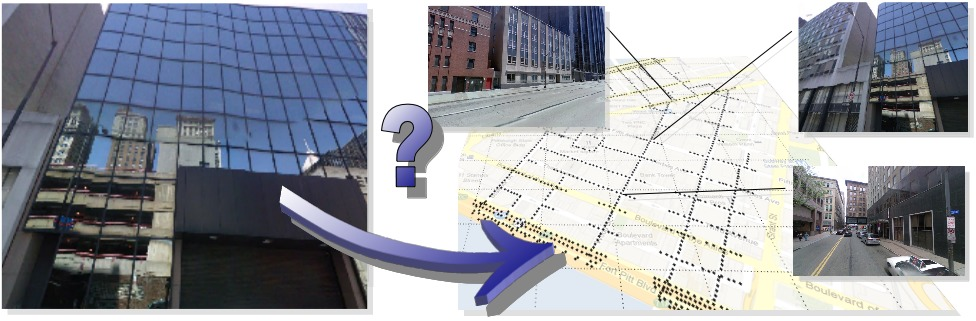
\includegraphics[width=.85\textwidth]{imgs/titleTeX.jpg}
        \vspace*{-3mm}
        \captionof{figure}
        {
          The goal of this work is to localize a query photograph (left) by finding other images of the same place in a large geotagged image database (right). 
          We cast the problem as a classification task and learn a classifier for each location in the database. 
          We develop two procedures
          to calibrate the outputs of the large number of per-location classifiers without the need for additional labelled training data.                     
%          We develop a non-parametric \textcolor{myGrey}{(can we asy tis for FV w-norm norm?)} procedure to calibrate the outputs of the large number of per-location classifiers without the need for additional positive training data.  
        }
    \end{center}%
}]
% ******************************************************

%\maketitle

\begin{abstract}
The aim of this work is to localize a query photograph by finding other images depicting the same place in a large geotagged image database. 
This is a challenging task due to changes in viewpoint, imaging conditions and the large size of the image database. The contribution of this work is two-fold. First, we cast the place recognition problem as a classification task and use the available geotags to train a classifier for each location in the database in a similar manner to per-exemplar SVMs in object recognition. 
Second, as only few positive training examples are available for each location, we propose 
two methods to calibrate all the per-location SVM classifiers without the need for additional positive training data.
The first method relies on p-values from statistical hypothesis testing and uses only the available negative training data. The second method performs an affine calibration by appropriately normalizing the learnt classifier hyperplane and does not need any additional labelled training data.
We test the proposed place recognition method with the bag-of-visual-words and Fisher vector image representations suitable for large scale indexing. 
Experiments are performed on a database of 25,000 geotagged street view images of Pittsburgh and demonstrate improved place recognition accuracy of the proposed approach over the previous work.
% Add SF: as well as the San Francisco dataset containing 1M geotagged images
%\textcolor{myGrey}{
%Second, as only few positive training examples are available for each location, we propose a new approach to calibrate all the per-location SVM classifiers using \emph{only} the negative examples. The calibration we propose relies on a significance measure essentially equivalent to the p-values classically used in statistical hypothesis testing. Experiments are performed on a database of 25,000 geotagged street view images of Pittsburgh and demonstrate improved place recognition accuracy of the proposed approach over the previous work.
%\emph{(FV calibration)}}
\keywords{Place recognition \and SVM calibration \and Geo-location}
% \PACS{PACS code1 \and PACS code2 \and more}
% \subclass{MSC code1 \and MSC code2 \and more}
\end{abstract}
%%%%%%%%%%%%%%%%%%%%%%%%
\section{Introduction}
%%%%%%%%%%%%%%%%%%%%%%%%
   \label{intro}
   Visual place recognition~\cite{Cummins09,Knopp2010,Schindler07} is a challenging task as the query and database images may depict the same 3D structure (e.g.\ a building) from a different camera viewpoint, under different illumination, or the building can be partially occluded. 
   In addition, the geotagged database may be very large. For example, we estimate that Google street-view of France alone contains more than 60 million panoramic images.
It is, however, an important problem as automatic, accurate and fast visual place recognition would have many practical applications in robotics, augmented reality or navigation.

  Similar to other work in large scale place recognition~\cite{Cummins09,Knopp2010,Schindler07,Torii2013} and image retrieval~\cite{Nister06,Philbin07,Sivic2003,Jegou12} we describe each image by a set of local invariant features~\cite{Bay06,Lowe04}
%  , such as SURF~\cite{Bay06} or SIFT~\cite{Lowe04} 
  that are encoded and aggregated into a fixed-length single vector descriptor for each image. In particular, in this work we consider the sparse tf-idf weighted bag-of-visual-words representation~\cite{Sivic2003,Philbin07} and the compact Fisher vector descriptors~\cite{Jegou12}.  
%  Each image is then represented by a weighted histogram of visual words, called the ``tf-idf vector'' due to the commonly used tf-idf weighting scheme~\cite{Sivic2003}. 
The resulting vectors are then normalized to have unit $L_2$ norm and the similarity between the query and a database vector is measured by their dot product. This representation has some desirable properties such as robustness to background clutter and partial occlusion. Efficient retrieval is then achieved using inverted file indexing.

%   Similar to other work in large scale place recognition~\cite{Cummins09,Knopp2010,Schindler07} and image retrieval~\cite{Nister06,Philbin07,Sivic2003}, we build on the bag-of-visual-words representation~\cite{Csurka04,Sivic2003} and describe each image by a set of quantized local invariant features, such as SURF~\cite{Bay06} or SIFT~\cite{Lowe04}.  Each image is then represented by a weighted histogram of visual words, called the ``tf-idf vector'' due to the commonly used tf-idf weighting scheme~\cite{Sivic2003}. The vectors are usually normalized to have unit $L_2$ norm and the similarity between the query and a database vector is then measured by their dot product. This representation has some desirable properties such as robustness to background clutter and partial occlusion. Efficient retrieval is then achieved using inverted file indexing. 

%   Recent work has looked at different ways to improve the retrieval accuracy and speed of the bag-of-visual-words model for image and object retrieval. Examples include: 
%   (i) learning better visual vocabularies from training examples with matched/non-matched descriptors~\cite{Mikulik2010,Philbin10b}; 
%   (ii)  developing quantization methods less prone to quantization errors~\cite{Jegou2011,Philbin08} or 
%   (iii) combining results from multiple query images depicting the same scene~\cite{Chum11,Chum07b}.

   While in image retrieval  databases are typically unstructured collections of images, place recognition databases are usually structured: images have geotags, are localized on a map and depict a consistent 3D world. %~\cite{Gronat2011}. 
   Knowing the structure of the database can lead to significant improvements in both speed and accuracy of place recognition. 
   Examples include: (i) building an explicit 3D reconstruction of the scene~\cite{Irschara2009,Li10,Li12}; (ii) constructing an image graph~\cite{Cao13,Philbin10c,Turcot09}, where images are nodes and edges connect close-by images on the map~\cite{Torii11}, or (iii) using the geotagged data as a form of supervision to select local features that characterize a certain location~\cite{Knopp2010,Schindler07} or re-rank retrieved images~\cite{Zamir10}.

   In this work, we also take advantage of geotags as an available form of supervision and investigate whether the place recognition problem can be cast as a classification task.
   While visual classifiers were investigated for landmark \cite{Li09} recognition in consumer photo collections, where many photographs are available for each landmark, in this work we wish to train a classifier {\em for each location on the map} in a similar manner to per-exemplar classification in object recognition~\cite{Malisiewicz11}. This is beneficial as  each classifier can learn which features are discriminative for a particular place. % and down-weight features occurring at other places.
   The classifiers are learnt offline. At query time, the query photograph is localized by transferring the GPS tag of the best scoring location classifier.

   While learning classifiers for each place may be appealing, calibrating outputs of the individual classifiers is a critical issue. In object recognition~\cite{Malisiewicz11}, it is addressed in a separate calibration stage on a held-out set of training data.
   This is not possible in the place recognition set-up as only a small number, typically one to five, of positive training images are available for each location (e.g. street-view images viewing the same building facade). To address this issue, we propose two calibration methods. 
The first method relies on p-values from statistical hypothesis testing and uses only the available negative training data. The second method performs a simple affine calibration by appropriately normalizing the learnt classifiers and does not need any additional labelled calibration examples.   
%   The first calibration procedure is inspired by the use of p-values in statistics and is based on ranking the score of a query image amongst scores of other images in the database. The second method can be interpreted as a special case of affine calibration that relies only on learned SVM weight.
%   The rest of the paper is organized as follows: Section~\ref{sec:classifiers} describes how per-location classifiers are learnt. Sections~\ref{sec:calibration}~and~\ref{sec:calibrationRenorm} detail the classifier calibration procedure.   Implementation details and experimental results are given in Section~\ref{sec:experiments}.

%%%%%%%%%%%%%%%%%%%%%%%%%%%%%%%%%
\section{Related work} 
\label{sec:related}
%%%%%%%%%%%%%%%%%%%%%%%%%%%%%%%%%

\paragraph{Large-scale visual place recognition.}
    The visual localization problem is typically treated as large-scale instance-level retrieval~\cite{Cummins09,Chen11,Gronat13,Knopp2010,Schindler07,Torii2013,Zamir10}, where images are represented using local invariant
    features~\cite{Lowe04} encoded and aggregated into the bag-of-visual-words~\cite{Csurka04,Sivic03} or Fisher vector~\cite{Jegou12} representations. 
    The image database can be further augmented by 3D point clouds~\cite{Klinger13}, automatically
    reconstructed by large-scale structure from motion
    (SfM)~\cite{Agarwal-ICCV-2009,Klinger13}, which enables accurate prediction of query image camera position~\cite{Li12,Sattler12}.
    In contrast, in this work we investigate learning a discriminative place-specific image representation. A similar idea has been recently explored in~\cite{Cao13} 
    who learn a graph-based discriminative representation for landmark image collections where typically many images are available for each place.
%    For the Fisher vector image representation, other recent work~\cite{Simonyan2013} has demonstrated improved performance in a face recognition application by finding discriminative projection using a large amount of labelled training face data.     
    In this work, we focus on street-level images such as Google street-view, which have greater coverage, but typically only one or a small number of images are  available for each place.  To address this issue we learn a discriminative re-weighting of the descriptor specific to each image in the database using per-exemplar support vector machine~\cite{Malisiewicz11}.
    
    
%     using both the bag-of-visual-words representation as well as the compact Fisher vector descriptors~\cite{Jegou12}.  
%    Fisher vector descriptors have shown excellent place recognition accuracy~\cite{Torii2013}. In this work we further
%    improve their performance by discriminative learning.
%    %or more recently~\cite{Torii-CVPR-2013} the Fisher vector
    %descriptor~\cite{Jegou12}.  

%\paragraph{Fisher vector image representations} \vspace{-3mm}
%    Fisher vector image representations have recently demonstrated excellent performance for a number of visual recognition tasks~\cite{Chatfield11,Jegou12,Krapac2011,Simonyan2013}.
%    They are specially suited for retrieval applications since they are robust to image appearance variations and capture richer image statistics than the simple bag-of-visual-words (BOW) aggregation. However, raw extracted Fisher vectors are typically high-dimensional, e.g.\ with 32,768 non-sparse dimensions, which is impractical for large-scale visual recognition and indexing applications. Hence, their dimensionality is often reduced by principal component analysis (PCA) and further quantized for efficient indexing using, e.g.\, a product quantizer~\cite{Jegou12}.  Other recent work has demonstrated improved performance in a face recognition application by finding discriminative projection using a large amount of training face data~\cite{Simonyan2013}. Our work is complementary to these methods as it operates on the projected low-dimensional descriptor and further learns discriminative re-weighting of the descriptor specific to each image in the database using per-exemplar support vector machine~\cite{Malisiewicz11}.

\paragraph{Per-exemplar support vector machine.} 
    The exemplar support vector machine (w-norm) has been used in a number of visual recognition tasks including
    category-level recognition~\cite{Malisiewicz11}, cross-domain retrieval~\cite{Shrivastava11}, scene parsing~\cite{Tighe13}, %image to 3D model alignment~\cite{Aubry13},
    place recognition~\cite{Gronat13} or as an initialization  for more complex discriminative clustering models~\cite{Doersch12,Singh12}. The main idea is to train a linear support vector machine (SVM) classifier from a single positive example and a large number of negatives. The intuition is that the resulting weight vector will give a higher weight to the discriminative dimensions of the positive training data point and will down weight dimensions that are non-discriminative with respect to the negative training data. A key advantage is that each per-exemplar classifier can be trained independently and hence the learning can be heavily parallelized. 
    The per-exemplar training brings however also an important drawback. As each classifier is trained independently a
    careful calibration of the resulting classifier scores is required~\cite{Malisiewicz11}. 

\paragraph{Calibrating classifier scores.} 
 Several calibration approaches have been proposed in the literature (see~\cite{gebel2007calibrating} and references therein for a review). The most known consists of fitting a logistic regression to the output of the SVM~\cite{Platt99}.  This approach, however, has a major drawback as it imposes a parametric form (the logistic a.k.a.\ sigmoid function) of the likelihood ratio of the two classes, which typically leads to biased estimates of the calibrated scores. Another important calibration method is the isotonic regression~\cite{zadrozny2002transforming}, which allows for a non-parametric estimate of the output probability.
   Unfortunately, the fact that we have only a single positive example
   (or only very few of them, and which are all used for training)
    essentially prevents us from using any of these methods. 
To address these issues, we develop two classifier calibration methods that do not need additional labelled positive examples.
Related to ours is also the recent work of Scheirer et al.~\cite{Scheirer12} who develop a classifier calibration method for face attribute similarity search.
Their method (discussed in more detail in section~\ref{sec:calibration}) also does not require labelled positive examples but, in contrast to us, uses a parametric model (the Weibull distribution) for the scores of negative examples.    


\paragraph{Contributions.} 
This paper has two main contributions. First, we cast the place recognition problem as a classification task and use the available geo-tags to train a classifier for each location in the database (section~\ref{sec:classifiers}). Second, as only few positive training examples are available for each location, we propose two methods to calibrate all the per-location SVM classifiers without the need for additional positive training data. The first method (section~\ref{sec:calibration}) relies on p-values from statistical hypothesis testing. The second method (section~\ref{sec:calibrationRenorm}) performs an affine calibration by appropriately normalizing the learnt decision hyperplane. 
We also describe a memory efficient classifier representation for the sparse bag-of-visual-word vectors (section~\ref{sec:memory}) and experimentally demonstrate benefits
of the proposed approach (section~\ref{sec:experiments}). 

%    The contributions of this work are threefold.    
%    First, we analyze the exemplar support vector machine objective and show that the learnt hyperplane can be interpreted
%    as a new descriptor that replaces the original positive example and is re-weighted to increase its separation from the negative data.
%    Second, we demonstrate that after an appropriate normalization of the new re-weighted descriptor no further calibration is necessary. 
%    Third, we apply w-norm training to compact Fisher vector descriptors for large-scale place recognition resulting in  
%    a {\em discriminative} yet {\em compact} representation of each image in the database. 
%    Place recognition results are shown on two image datasets from Pittsburgh and demonstrate the learnt representation
%    consistently improves over the standard Fisher vector descriptors at different target dimensions. % with different dimensions. 




%%%%%%%%%%%%%%%%%%%%%%%%
\section{Per-location classifiers for place recognition}
\label{sec:classifiers}
%%%%%%%%%%%%%%%%%%%%%%%%
%  \textcolor{myGrey}{
%  This section (and almost the whole paper) implicitly speaks about tf-idf. However, there will be a section about FV later. We should re-design this section to be more general. We can keep \emph{Dual representaton} outside as separate section related to tf-idf.
%  } \newline
   We are given an image descriptor $\vec{x_j}$, one for each database image $j$. This representation can be a sparse tf-idf weighted bag-of-visual-words vector~\cite{Sivic03} or a dense compact descriptor such as the Fisher vector (FV)~\cite{Jegou12}. The goal is to learn a score $f_j$ for each database image $j$, so that, at test time, given the descriptor $\vec{q}$ of the query image, we can either retrieve the correct target image as the image $j^*$ with the highest score 
   \begin{equation}
   \label{eq:class}
    j^*=\operatorname*{arg\;max}_{j} f_j(\vec{q}) 
   \end{equation}

   \noindent
   or use these scores to rank candidate images and use geometric verification to identify the correct location in an $n$-best list.
   Instead of approaching the problem directly as a large multiclass classification problem, we tackle the problem by learning a per-exemplar linear SVM classifier~\cite{Malisiewicz11}  for each database image $j$.
   Similar to~\cite{Knopp2010}, we use the available geotags to construct the negative set $\mathcal N_j$ for each image $j$. The negative set is constructed so as to concentrate difficult negative examples, i.e.\ from images that are far away from the location of image $j$ and at the same time similar to the target image as measured by the dot product between their feature vectors. The details of the construction procedure will be given in section~\ref{sec:experiments}.  The positive set $\mathcal P_j$ is represented by the only positive example, which is $\vec{x_j}$ itself. 
   Each SVM classifier produces a score $s_j$ which is a priori not comparable with the score of the other classifiers. A calibration of these scores will therefore be key to convert them to comparable scores $f_j$. This calibration problem is more difficult than usual given that we only have a single positive example and will be addressed in section~\ref{sec:calibration}.
   
   %%%%%%%%%%%%%%%%%%%%%%%%%%%%%%%%%%%%%%%%%%%%%%%%%%%
   \subsection{Learning per-location SVM classifiers }
   %%%%%%%%%%%%%%%%%%%%%%%%%%%%%%%%%%%%%%%%%%%%%%%%%%%
      Each linear SVM classifier learns a score $s_j$ of the form 

      \begin{align}
        s_j(\vec{q})=\vec{q}^T \vec{w_j}+b_j
        \label{eq:linear}
      \end{align}

      \noindent
      where $\vec{w_j}$ is a weight vector re-weighting contributions of individual visual words and $b_j$ is the bias specific for image $j$. Given the training sets $\mathcal P_j$ and $\mathcal N_j$, the aim is to find a vector $\vec{w_j}$ and bias $b_j$ such that the score difference between $\vec{x_j}$ and the closest neighbor from its negative set $\mathcal N_j$ is {\em maximized}. % modulo margin (perhaps mention this).
      Learning the weight vector $\vec{w_j}$ and bias $b_j$ is formulated as a minimization of the convex objective 
      \begin{align}
        \nonumber
        \Omega(\vec{w_j},b_j)=||\vec{w_j}||^{2}& +C_1\sum_{\vec{x}\in \mathcal P_j}h(\vec{w_j}^T\vec{x}+b_j)   \\
        \label{eq:obj}
                           & +C_2\sum_{\vec{x}\in \mathcal N_j}h(-\vec{w_j}^T\vec{x}-b_j), 
      \end{align}

      \noindent
      where the first term is the regularizer, the second term is the loss on the positive training data weighted by scalar parameter $C_1$, and the third term is the loss on the negative training data weighted by scalar parameter $C_2$.   
      This is a standard SVM formulation \eqref{eq:obj}, also used in exemplar-SVM~\cite{Malisiewicz11}.
      In our case $h$ is the squared hinge loss, which we found to work better in our setting than the standard hinge-loss. $\vec{w_j}$ and $b_j$ are learned separately for each database image $j$ in turn. 
%      \sout{
%      In our case (details in section~\ref{sec:experiments}), we use about 1-5 positive examples, and 200 negative examples. As the dimensionality of $\vec{w}$ is $100,000$ all training data points are typically support vectors. 
%      }
%      \textcolor{myGrey}{
%        \emph{(Above we claim that only a single positive is available)}
%      }
   % %%%%%%%%%%%%%%%%%%%%%%%%%%%%%%%%%%%%%%%
   % \paragraph{Expanding the positive set.}
   % %%%%%%%%%%%%%%%%%%%%%%%%%%%%%%%%%%%%%%%
   %    \sout{
   %    A typical geotagged database may contain several images depicting a particular location. For example, neighboring street-view panoramas depict the same store front from different viewpoints. However, a specific place is often imaged only in a small number (2-5) of neighboring panoramas. 
   %    If such images are identified, they may provide a few additional positive examples for the particular place and improve the quality of that per-location classifier. Moreover, treating them erroneously as negatives is likely to bias the learnt classifier.
   %    We automatically identify such images as geo-graphically close-by images to the location $j$.
   %    These images can be further verified using geometric verification~\cite{Philbin07} and included in the positive training data for location $j$. Details are given in section~\ref{sec:experiments}.
   %    }
      

   \subsection{The need for calibrating classifier scores}
   Since the classification scores $s_j$ are learned independently for each location $j$, they cannot be directly used for place recognition as in eq.~\eqref{eq:class}. As illustrated in figure~\ref{fig:calib}, for a given query $q$, a classifier from an incorrect location (b) can have a higher score~\eqref{eq:linear} than the classifier from the target location (a). Indeed, the SVM score is a signed distance from the discriminating hyperplane and is a priori not comparable between different classifiers. This issue is addressed by calibrating scores of the learnt classifiers. The goal of the calibration is to convert the output of each classifier into a probability (or in general a ``universal" score), which can be meaningfully compared across classifiers. In the following two sections we develop two classifier calibration methods that do not need additional labelled positive examples.


%   Several calibration approaches have been proposed in the literature (see~\cite{gebel2007calibrating} and references therein for a review). The most known consists of fitting a logistic regression to the output of the SVM~\cite{Platt99}.  This approach, however, has a major drawback as it imposes a parametric form (the logistic a.k.a.\ sigmoid function) of the likelihood ratio of the two classes, which typically leads to biased estimates of the calibrated scores. Another important calibration method is the isotonic regression~\cite{zadrozny2002transforming}, which allows for a non-parametric estimate of the output probability.
%   Unfortunately, the fact that we have only a single positive example
%   (or only very few of them, and which are all used for training)
%    essentially prevents us from using any of these methods. 
%To address these issues, in the following two sections we develop two classifier calibration methods that do not need additional labelled positive examples.

%In the first method (Section~\ref{}) we exploit the the availability of large amounts of negative data, i.e.\ images from other far away locations in the database.
%In particular, we estimate the significance of the score of a test example compared to the typical score of  the (plentifully available) negative examples. Intuitively, we will use a large dataset of negative examples to calibrate the individual classifiers so that they {\em reject the same number of negative examples} at each level of the calibrated score.   We will expand this idea in detail and use concepts from hypothesis testing to propose a calibration method.

%In the second method (Section~\ref{}), ... 

%   However, given the availability of negative data, it is easy to estimate the significance of the score of a test example compared to the typical score of (plentifully available) negative examples. Intuitively, we will use a large dataset of negative examples to calibrate the individual classifiers so that they {\em reject the same number of negative examples} at each level of the calibrated score.
%   We will expand this idea in detail and use concepts from hypothesis testing to propose a calibration method.

    
%%%%%%%%%%%%%%%%%%%%%%%%%%  
\section{Non-parametric calibration of the  SVM-scores from negative examples only}
\label{sec:calibration}
%%%%%%%%%%%%%%%%%%%%%%%%%%  

In this section we describe a classifier calibration method that exploits the availability of large amounts of negative data, i.e.\ images from other far away locations in the database.
In particular, the method estimates the significance of the score of a test example compared to the typical score of  the (plentifully available) negative examples. Intuitively, we will use a large dataset of negative examples to calibrate the individual classifiers so that they {\em reject the same number of negative examples} at each level of the calibrated score.   We will expand this idea in detail using the concepts from hypothesis testing. % to propose a calibration method.
   %%%%%%%%%%%%%%%%%%%%%%%%%%%%%%%%%%%%%%%%%%%%%%%%%%%%%%%
   \subsection{Calibration \emph{via} significance levels}
   %%%%%%%%%%%%%%%%%%%%%%%%%%%%%%%%%%%%%%%%%%%%%%%%%%%%%%% 
      In the following, we view  the problem of deciding whether a query image matches a given location based on the corresponding SVM score as a hypothesis testing problem. In particular, we appeal to ideas from the traditional frequentist hypothesis testing framework also known as Neyman-Pearson (NP) framework (see e.g.~\cite{casella2001statistical}, chap.~8).

      We define the null hypothesis as $H_0=\{$the image is a random image$\}$ and the alternative as $H_1=\{$the image matches the particular location$\}$. The NP framework focuses on the case where the distribution of the data under $H_0$ is well known, whereas the distribution under $H_1$ is not accessible or too complicated to model, which matches perfectly our setting.
%      \textcolor{myGrey}{How about the other NP assumptions? We should ask Guillaume}

      In the NP framework, the \emph{significance level} of a score is measured by the p-value or equivalently by the value of the cumulative density function  (cdf) of the distribution of the negatives at a given score value. The cdf is the function $F_0$ defined by $F_0(s)=\PP(S_0\leq s)$, where $S_0$ is the random variable corresponding to the scores of negative data (see figure~\ref{fig:qntExample} for an illustration of the relation between the cdf and the density of the function). The cdf 
      (or the corresponding p-value\footnote{
        The notion most commonly used in statistics is in fact the p-value. The p-value associated to a score is the quantity $\alpha(s)$ defined by $\alpha(s)=1-F_0(s)$; so the more significant the score is, the closer to $1$ the cdf value is, and the closer to $0$ the p-value is. To keep the presentation simple, we avoid the formulation in terms of p-values and we only talk of the probabilistic calibrated values obtained from the cdf $F_0$.
       }%
       )
      is naturally estimated by the empirical cumulative density function $\hat{F}_0$, which is computed as: 
      
      \begin{equation}
        \hat{F}_0(s)=\frac{1}{\Ncal} \sum_{n=1}^{\Ncal} 1_{\{s_n \leq s\}},
        \label{eq:empiricalCDF}
      \end{equation}

      \noindent
      where $(s_n)_{1\leq n \leq \Ncal }$ are the SVM scores associated with $\Ncal$ negative examples used for calibration.
      $\hat{F}_0(s)$ 
      is the fraction of the negative examples used for calibration (ideally held out negative examples) that have a score below a given value $s$.
      Computing $\hat{F}_0$ exactly would require to store all the SVM scores for all the calibration data for all classifiers, so in practice, we only keep a fraction of the larger scores.
      We also interpolate the empirical cdf between consecutive datapoints so that instead of being a staircase function it is a continuous piecewise linear function such as illustrated on figure~\ref{fig:calib}. Given a query, we first compute its SVM score $s_q$ and then compute the calibrated probability $f(q)=\hat{F}_0(s_q)$.
      We obtain a similar calibrated probability $f_j(q)$ for each of the SVMs associated with each of the target locations, which can now be ranked.

      \begin{figure}[t]
         \vspace{1mm}
         \subfigure[]{
            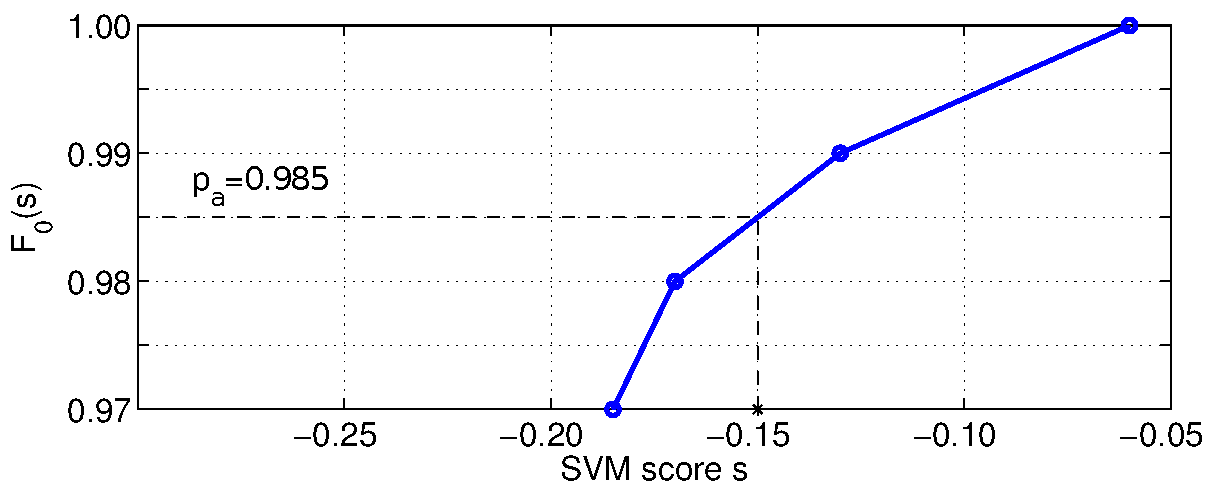
\includegraphics[width=\linewidth]{imgs/qnt1x}
            \label{fig:subfig1}
         }
         \vspace{1.5mm}\newline
         \subfigure[]{
            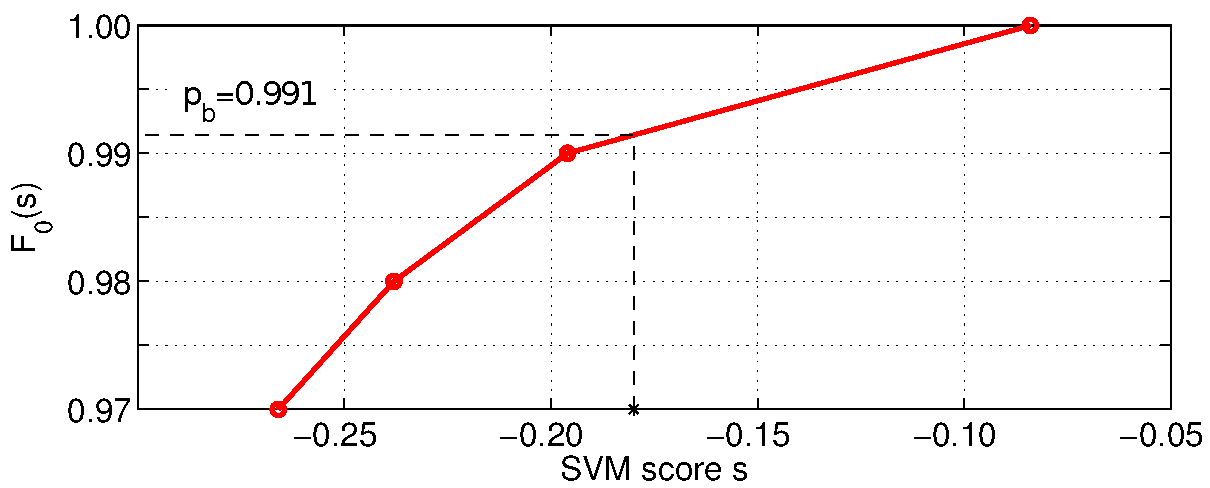
\includegraphics[width=\linewidth]{imgs/qnt2x}
            \label{fig:subfig2}
         }
         \vspace*{-3mm}
         \caption[]{
            An illustration of the proposed normalization of SVM~scores for two different database images. In each plot, the x-axis shows the raw SVM score. The y-axis shows the calibrated output. For the given query, the raw SVM score of image (b) is lower than for image (a), but the calibrated score of image (b) is higher than for image (a). 
         }
         \vspace*{-2mm}
         \label{fig:calib}
      \end{figure}

      \begin{figure}[t]
         \subfigure[]{
            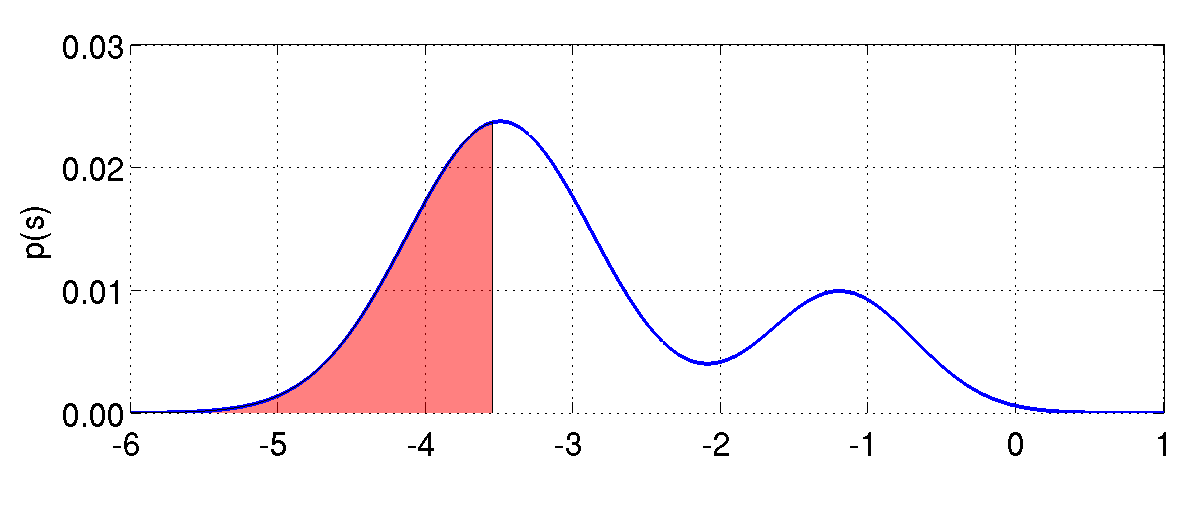
\includegraphics[width=\linewidth]{imgs/qntEx1.pdf}
         }
         \subfigure[]{
            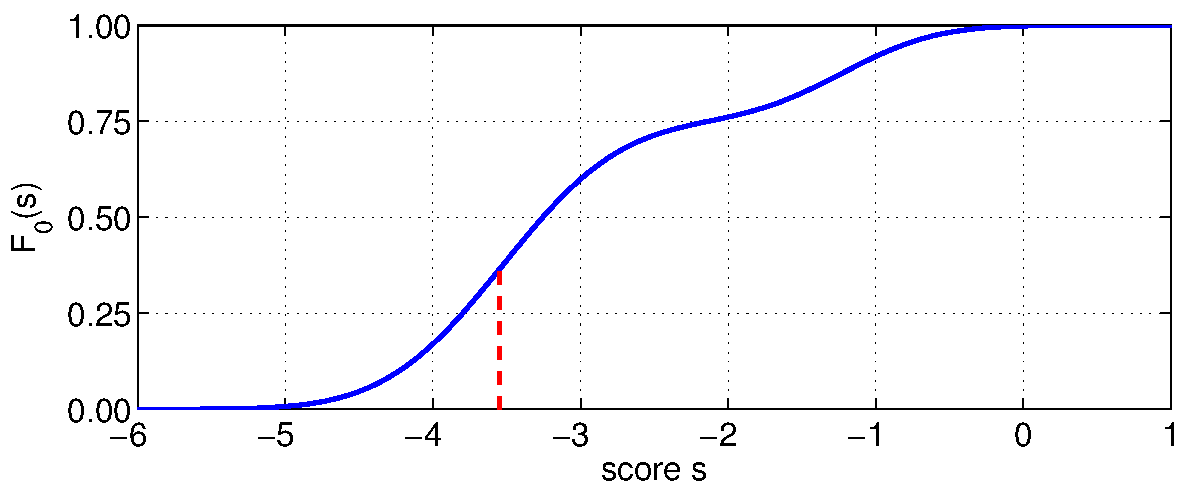
\includegraphics[width=\linewidth]{imgs/qntEx2.pdf}
         }
         \vspace*{-3mm}
         \caption{Illustration of the relation between (a) the probability density of the random variable $S_0$ modeling the scores of the negative examples and (b) the corresponding cumulative density function $F_0(s)=\PP(S_0 \leq s)$.
         }
               \vspace*{-3mm}
         \label{fig:qntExample}
      \end{figure}
      
      
   %%%%%%%%%%%%%%%%%%%%%%%%%%%%%%%%%%%%%%%%%%%%%%%%%
   \subsection{Summary of the calibration procedure}
   %%%%%%%%%%%%%%%%%%%%%%%%%%%%%%%%%%%%%%%%%%%%%%%%%
    
    For each trained place-specific classifier $s_j$ we construct the empirical cumulative density function~\eqref{eq:empiricalCDF} of scores of the negative examples and keep only its top $K$ values. This can be done offline and the procedure is summarized in Algorithm \ref{alg:offline}. 
    %
    At query time, given a query image descriptor $\vec{q}$, we compute the uncalibrated classification score $s_j(\vec{q})$ and then use the stored cdf values to compute the calibrate score $f_j(\vec{q})$. This procedure is performed for each database image $j$ and is summarized in Algorithm \ref{alg:online}.
    Finally, the best candidate database image is selected by equation~\eqref{eq:class}. Alternatively, candidate database images can be also ranked according to the calibrated score.
 
% {\tt TODO: Petre, the algorithms are a bit confusing as you suddently introduce a completely new notation different that is the main text.
% Could you please make the notation consistent? I.e. the algorithms should use the s, F, f as in the main text.  Please also include explicitly the equation for interpolation
% as suggested in the Algorithm 2. As suggested in the algorithm, 
% } 
 
 
      \begin{algorithm}
         \caption{P-value calibration: offline stage}\label{alg:offline}
         \begin{algorithmic}[1]
         \Procedure{p-value calibration}{}
         \State $N \gets$ database size
         %\State $K \gets$ size of the cdf tail to be kept
         \State $\mathcal{X} \gets$ descriptor matrix of negative examples %all database images
         \For{$\forall j \in 1 \dots N$}
            \State $N_c \gets$ number of negative examples
            \State $\vec{w} \gets$ learned SVM weight for image $j$
            \State $b \gets$ learned SVM bias for image $j$
            \State $\vec{\sigma} \gets \vec{w}^T \mathcal{X}+b$
            \State {\em Compute the cdf:}  % $\vec{s_j}, \hat{F}_{0j}$ }
            \State $\vec{s_j} \gets$ sorted $\vec{\sigma}$ in descending order
            \State $\hat{F}_{0j} \gets [N_c \dots 0]/N_c$
         \EndFor
         \EndProcedure
         \end{algorithmic}
         \label{alg:onffline}
      \end{algorithm}

       \begin{algorithm}
         \caption{P-value calibration: online stage}\label{alg:online}
         \begin{algorithmic}[1]
         \Procedure{calibrating scores}{}
         \State $\vec{q} \gets$ query image descriptor
         \State $N \gets$ database size
%         \State $y \gets [0,1,\dots (K-1)]$
         \For{$\forall j \in 1 \dots N$} // for each database image
            \State $\vec{w} \gets$ learned SVM weight for image $j$
            \State $b \gets$ learned SVM bias for image $j$
            \State $\hat{F}_{0} \gets \hat{F}_{0j}$ // Empirical cdf
            \State $\vec{s} \gets \vec{s_j}$ // Corresponding sorted scores
            \State $s_q \gets \vec{q}^T\vec{w}+b$  // compute uncalibrated classifier score 
%		        \State $\hat{F}_0 \gets \hat{F}_{0j}$
            \State Find $n$ such that $s_{n} \leq s_q < s_{n+1} $
            \State Compute the interpolated empirical cdf value:
            \Statex $\hspace{9mm}
              \hat{F}_0(s_q)\approx 
              \hat{F}_0(s_n)+\frac{s_q-s_n}{s_{n+1}-s_n} (\hat{F}_0(s_{n+1})-\hat{F}_0(s_n)).
            $
            \State $f_j(\vec{q})=\hat{F}_0(s_q)$ // output the calibrated score
         
         \EndFor
         \EndProcedure
         \end{algorithmic}
         \label{alg:online}
      \end{algorithm}
      
%             \begin{algorithm}
%         \caption{P-value calibration: online stage}\label{alg:online}
%         \begin{algorithmic}[1]
%         \Procedure{calibrating scores}{}
%         \State $\vec{q} \gets$ query image descriptor
%         \State $T \gets$ length of the output shortlist
%         \State $N \gets$ database size
%         \State $K \gets$ size of the kept cdf tail
%%         \State $y \gets [0,1,\dots (K-1)]$
%         \For{$\forall j \in 1 \dots N$} // for each database image
%            \State $\vec{w} \gets$ learned SVM weight for image $j$
%            \State $b \gets$ learned SVM bias for image $j$
%            \State $s \gets \vec{q}^T\vec{w}+b$  // compute uncalibrated classifier score
%%            \State $x \gets calib_j$
%            \If{$s>calib_j[1]$}
%               \State $idx \gets 0$ \hspace{10mm} // score below stored c.d.f. values
%            \ElsIf{$calib_j[K]>s$}
%               \State $idx \gets 1$ \hspace{9mm} // score above stored c.d.f. values 
%            \Else
%  		\State Find $n$ such that $s_{n} \leq s_q < s_{n+1} $
%		\State 
%         $
%         \hat{F}_0(s_q)\approx 
%         \hat{F}_0(s_n)+\frac{s_q-s_n}{s_{n+1}-s_n} (\hat{F}_0(s_{n+1})-\hat{F}_0(s_n)).
%        $\\
%%            \State $f[j] \gets (N-idx)/N$ \hspace{10mm} // p-value $\in (0..1)$
%              % \State $idx \gets interpolate(x,y,s)$
%            \EndIf
%            
%         \EndFor
%         \EndProcedure
%         \end{algorithmic}
%         \label{alg:online}
%      \end{algorithm}

      % For each place, keep $\Ncal$ scores from negative examples~$(s_n)_{1 \leq n \leq \Ncal}$ used for calibration together with the associated cumulative probability values $\hat{F}_0(s_n)$.
      % Given the score of the query $s_q$:\\
      % 1.  Find $n$ such that $s_{n} \leq s_q < s_{n+1} $\\
      % 2.  Compute the interpolated empirical cdf value
      % \begin{equation}
      %   \hat{F}_0(s_q)\approx 
      %   \hat{F}_0(s_n)+\frac{s_q-s_n}{s_{n+1}-s_n} (\hat{F}_0(s_{n+1})-\hat{F}_0(s_n)).
      %   \label{eq:interp}
      % \end{equation}

   %%%%%%%%%%%%%%%%%%%%%%%
   \subsection{Discussion.}
   %%%%%%%%%%%%%%%%%%%%%%% 
      It should be noted that basing the calibration only on the negative data has the advantage that we privilege precision over recall, which is justified given the imbalance of the available training data (much more negatives than positives).
      Indeed, since we are learning with a single positive example, intuitively, we cannot guarantee that the learned partition of the space will generalize well to other positives, whose scores in the test set can potentially drop significantly (this is indeed what we observe in practice). By contrast, since we are learning from a comparatively large number of negative examples, we can trust the fact that new negative examples will stay in the half-space containing the negative training set, so that their scores are very unlikely to be large. Our method is therefore based on the fact that we can measure reliably how surprising a high score would be if it was the score of a negative example. This exactly means that we can control false positives (type I error) reasonably well but not false negatives (type II error or equivalently the power of our test/classifier), exactly as in the Neyman-Pearson framework.

      An additional reason for not relying on positive examples for the calibration in our case is that (even if we had sufficiently many of them) the positive examples that we collect using location and geometric verification from the geotagged database typically have illumination conditions that are extremely similar to each other and not representative of the distribution of test positives which can have very different illuminations. This is because of the controlled nature of the capturing process of geotagged street-level imagery (e.g.\ Google street-view) used for experiments in this work. Close-by images are typically captured at a similar time (e.g. on the same day)and under similar imaging conditions.

      Scheirer et al.~\cite{Scheirer12} propose a method, which is related to ours, and calibrate SVM scores by computing the corresponding cdf value of a Weibull distribution fitted to the top negative scores. The main difficulty is that the Weibull model should be fitted only to the tail of the distribution of the negatives, which is in general difficult to identify. As a heuristic, Scheirer et al. propose to fit the Weibul model to false positives (i.e. the negative samples classified incorrectly as positives). But in our case, most of the exemplar SVMs that we are training have $0$ false positives in a held out set, which precludes the application of their method. To avoid that issue our approach forgoes any parametric form of the distribution and instead relies directly on a standard non-parametric estimate of the cumulative density function.

      Finally, we should remark that we are not doing here calibration in the same sense of the word as the calibration based on logistic regression (or isotonic regression), since logistic regression estimates a probability of making a correct prediction by assigning a new data to class $1$, while we are estimating how unlikely it would be for a negative example to have such a high score. The calibration with either methods yields ``universal" scores in the sense that they are comparable from one SVM to another, but the calibrated values obtained from logistic regression are not comparable to the values obtained from our approach.

%%%%%%%%%%%%%%%%%%%%%%%%%%  
\section{Affine calibration by-normalizing the classification hyperplane}
%\section{Calibration by-normalization }
\label{sec:calibrationRenorm}
%%%%%%%%%%%%%%%%%%%%%%%%%%  
  
  The non-parametric calibration method described in the previous section has two computational disadvantages, which make it hard to scale-up to very large datasets. 
  % of more than 1M images.  
  First, the method requires storing the non-parametric model of the calibration function for each learned classifier. This has memory complexity 
  of $O(NK)$, where $N$ is the number of images (classifiers) in the database and $K$ the number of stored elements of the non-parametric model. For typical values of $K=1000$ and $N=1M$ this would require additional 4GB of memory, comparable to the size of the inverted index itself. Second, computing the cumulative density function requires applying all $N$ learnt classifiers to the entire set of negative examples, which has also size $N$. As a result computing the cdf has complexity $O(N^2)$, which becomes quickly infeasible already for datasets with $N$ larger than $100,000$. 
  
To address these issues we first describe an affine calibration model that approximates the tail of the cdf with a simple linear function defined by only two parameters: its slope and offset, greatly reducing the required storage.
%This greatly reduces the storage requirements and makes storing the calibration functions feasible for very large datasets.
Second, we show that the parameters of the affine calibration function can be obtained by-normalizing the learnt classification hyper-plane without applying the classifiers on the negative data and thus bringing down the computational complexity to $O(N)$.
As a result,  computing and storing the calibration functions becomes feasible for very large datasets with 1M images.
%This greatly reduces the storage and computational requirements and makes computing and storing the calibration functions feasible for very large (1M+) datasets.

%The calibration method described above requires storing a non-parametric model of the calibration function for each learned classifier. Later, the SVM score calibration must be performed online at query time. These two aspects increase a memory footprint and computational cost in both offline and online phase. 
%
%  If $K$ is a fraction of values of the empirical cumulative density function that is kept for each SVM, the additional memory footprint of $O(NK)$ is required to store all calibration functions for a database of size $N$. Typically we keep $K=1,000$ values for each c.d.f. for the database size of $N=50,000$. This requires additional $\sim 200$MB. For lager datasets this may be a key limitation. At query time, given the raw SVM score, one has to find nearest values of the calibration function and interpolate between them \eqref{eq:interp} for each database image in turn. This operation requires additional computational time.
%  %This yields a computational complexity of $O(N \log{K})$.
%  To construct a calibration function at offline phase $N$ SVM scores must be sorted for each database image in turn. When the merge sort is used the total complexity for entire database of the c.d.f. construction is $O(N^2 \log{N})$. This makes the calibration method hard to scale up.
%
%  In this section we, first, simplify the calibration by approximating the cumulative density function by an affine function and show that nor additional memory nor computational cost is required at query time. Second, we address the offline stage problem by introducing a calibration by-normalization and shift which reduces the offline complexity to $O(N)$.

   \subsection{Affine calibration model}
   Using the affine calibration model we transform the uncalibrated score $s_j(\vec{q})$ of query $\vec{q}$ with a linear function 
%     The main disadvantage of the \emph{p-value} calibration is the memory footprint and need for additional computation at query time. This can be eliminated by simplification of the calibration model. Each calibration function can be approximated by an affine line such that calibration function can be written as follows
     \begin{equation}
       f_j(\vec{q}) = \alpha_j s_j(\vec{q}) + \beta_j,
       \label{eq:affine}
     \end{equation}
	where 
%	$s_j(\vec{q})$ is the uncalibrated score for query $\vec{q}$ , 
	$ f_j(\vec{q})$ is the output calibrated score, and
	$\alpha_j$ and $\beta_j$ are scalar calibration parameters specific to each classifier $j$.
	In this work we use linear classifiers, hence substituting for $s_j(\vec{q})$ %in~\eqref{eq:affine} 
	the linear classifier from \eqref{eq:linear} results also in a linear calibrated classifier
%     \begin{align}
%%        \nonumber
%         f_j(\vec{q}) = c_j\vec{w}_j^T \vec{q}+ (c_j b_j+d_j)
%        %\label{eq:affine2}
%    \end{align}
%    that can be further simplified to
    \begin{align}
    \label{eq:linear2}
%      \nonumber
%        f_j(\vec{q}) = (c_j\vec{w}_j)^T \vec{q} + \beta_j
        f_j(\vec{q}) = \vec{\widetilde{w}}_j^T \vec{q} + c_j,
        %\label{eq:affiine3}
     \end{align}
    where $\vec{\widetilde{w}}_j = \alpha_j\vec{w}_j$ and $c_j=\alpha_j b_j+\beta_j$. 
    Note that the calibrated classifier~\eqref{eq:linear2} has the same form as the original classifier~\eqref{eq:linear} and hence this representation does not require any additional storage compared to storing the original classifier. %Compared to the~\cite{
    The question remains how to set the parameters $\alpha_j$ and $\beta_j$ of the calibration function~\eqref{eq:affine}, which is discussed next.
    
  
%    Setting the calibration parameters  
%    The parameters $c_j$ and $d_j$ of the calibration function 
    
    % As compared to (2) does not result in additional storage. 
    % How to set c and b? Can be done from data, but we do it directly.

%    While we have greatly reduced the storage complexity of the calibration to only two parameters.
%          The parameters $c_j$, $\beta_j$ in equation \eqref{eq:affine} represent an affine approximation the calibration function. 
%          Selection of these parameters still requires an expensive sorting of SVM scores for each database image in turn which yields a complexity of $O(N^2 \log{N})$ at offline phase.

    	
%     \noindent
%     Substituting for $s_j(\vec{q})$ from equation \eqref{eq:linear} into the equation above we get
%     \begin{align}
%        \nonumber
%         f_j(\vec{q}) = c_j\vec{w}_j^T \vec{q}+ (c_j b_j+d_j)
%        %\label{eq:affine2}
%    \end{align}
%
%    Notice that this can be further rewritten as a new affine function as follows
%    \begin{align}
%      \nonumber
%        f_j(\vec{q}) = (c_j\vec{w}_j)^T \vec{q} + \beta_j
%        %\label{eq:affiine3}
%     \end{align}
%
%    \noindent
%    where $\beta_j=c_j b_j+d_j$, which can be further written as a  dot product
%    \begin{equation}
%      f_j(\vec{q}) = \vec{\widetilde{q}}^T \vec{\widetilde{w}}_j
%      \label{eq:affiine3}
%    \end{equation}    
%     \noindent
%     where $\vec{\tilde{q}_j}=[\vec{q}_j^T 1]^T$ and $\vec{\widetilde{w}}_j = [\vec{w}_j^T \beta_j]^T$. The original score calibration requires expensive searching of nearest calibration values which yields complexity of $O(N \log{K} )$ at query time. Notice that the vector $\vec{\tilde{w}_j}$, consisting of scaled SVM weight and unity, can be computed offline. Therefore no additional memory storage or computational cost is required at query time and calibration. Since computing the raw SVM scores is $O(N)$ and $K$ is typically $1,000$ the online phase can be sped up by factor of $\log{K}\sim 10$.
%      The parameters $c_j$, $d_j$ in equation \eqref{eq:affine} represent an affine approximation the calibration function. Selection of these parameters still requires an expensive sorting of SVM scores for each database image in turn which yields a complexity of $O(N^2 \log{N})$ at offline phase.

   \subsection{Calibration by-normalization}
   Parameters of the affine calibration function~\eqref{eq:affine} could be learnt from negative training data in a similar manner to for example~\cite{Aubry14}. 
   However, as discussed above, in our case this would require running all $N$ classifiers on all $N$ images, which is prohibitive for large datasets.
   Instead, we have found that a good calibration can be obtained by-normalizing the learnt hyperplane $\vec{w}$. In particular, we set 
   %we found in practice good results can be obtained by setting 
   \begin{align}
   \label{eq:rescale1}
   \alpha_j &= \dfrac{1}{||\vec{w}_j||},\\ 
   \label{eq:rescale2}
    \beta_j &=  -b_j \alpha_j, 
   \end{align}
   where $\vec{w}_j$ and $b_j$ are the parameters of the learnt SVM hyper-plane for location $j$ and $||\vec{w}||$ is the $L_2$ norm of $\vec{w}$ . Given this choice of $\alpha_j$ and $\beta_j$
   the calibrated classification score~\eqref{eq:linear2} reduces to

      \begin{align}
%      \nonumber
%        f_j(\vec{q}) = (c_j\vec{w}_j)^T \vec{q} + \beta_j
        f_j(\vec{q}) = \dfrac{1}{||\vec{w}_j||}\vec{w}_j^T\vec{q}.
            \label{eq:linear3}
     \end{align}

     The intuition is that when $\vec{q}$ is $L_2$ normalized, equation~\eqref{eq:linear3} is equivalent to computing the normalized dot-product between vectors $\vec{q}$ and $\vec{w}$.       This was found to work well in image retrieval~\cite{Sivic03} or matching whitened HOG descriptors~\cite{Doersch13}.
%      but has not yet been used in conjunction with SVMs as done in this work.
In this work we investigate whether this intuition about descriptor matching can be used as a form of calibration for the learnt place-specific classifier.  
      Note  that this form of calibration by-normalization is scalable to very large datasets as it (i) requires only $O(N)$ computations offline to pre-compute the calibration parameters for each of the $N$ learnt classifiers (equations~\eqref{eq:rescale1} and~\eqref{eq:rescale2}), and (ii) does not need any additional storage or computation at query time as the calibration parameters can be included in the classifier~\eqref{eq:linear2}.   
%          We have found that this calibration works very well in practice when the SVM is appropriately regularized. In particular, we set parameters $C_1$ and $C_2$ in the SVM cost~\eqref{} by cross-validation to prevent overfitting to the single positive example and details are given in section~\ref{}.
      % - pluggin in 7+8 into 5 we see the form.
      % For L2 normalized descriptor this is equivalent to normalized scalar-product between the two vectors which was found to work well..
%  The intuition is that for an $L_2$ normalized query descriptor $\vec{q}$ computing the calibrated score $f_j(\vec{q})$ given by \eqref{eq:rescale1} and  \eqref{eq:rescale2}
   
  
%  corresponds to computing the normalized cross-correlation between vectors $w$ and $x$. This was found to work well in retrieval (see e.g. Sivic and Zisserman, \cite{}) or matching whitened HOG descriptors [11,13] \cite{}, \cite{} (see e.g. [Doersch et al., Mid-Level Visual Element Discovery as discriminative Mode Seeking, NIPS 2013] \cite{}), but has not yet been used in conjunction with SVMs as done in this work. Note also that the affine calibration can be computed offline and does not need any additional computation or storage at query time compared to the p-value calibration of \cite{Gronat13}.
%      Though the calibration by-normalization is simple we observe that this type of calibration is more suited for dense descriptors such as Fisher vectors. Details will be given next in the experimental section. 
%      
%      In the previous section we had to find parameters $c_j$ and $d_j$ from training data which can be still costly at training time and requires negative training data. Below we investigate whether it is possible to set $c_j$ and $b_j$ without any training. We found that this is possible by special choice of affine function based on learnt SVM. 
%      The raw SVM score can be calibrated such that, first, the bias term is subtracted and, second, the score is scaled by inverse of the SVM weight vector. The calibration function can be then written as follows
%      \begin{equation}
%         f_j(\vec{q}) = \dfrac{1}{||\vec{w}_j||}\vec{q}^T\vec{w}_j
%         \label{eq:rescale}
%      \end{equation}
%
%      \noindent
%      This calibration can be viewed as a spacial case of affine calibration where calibration parameters rely on SVM only. The equation \eqref{eq:rescale} can be further re-written as a dot-product
%      
%      \begin{equation}
%         f_j(\vec{q}) = \vec{q}^T\vec{\tilde{w}}_j
%         \label{eq:rescaled}
%      \end{equation}
%
%      \noindent
%      where $\vec{\tilde{w}}_j=\frac{\vec{\tilde{w}}_j}{||\vec{w}_j||}$ can be computed offline and yields only $O(N)$ complexity which allows the method to scale up.
%   
%   \subsection{Discussion}
%      We have found that this calibration works very well in practice when SVM is properly regularized.
%      The intuition is that for $L2$ normalized descriptors $x$ computing the calibrated score $f(x)$ corresponds to computing the normalized cross-correlation between vectors $w$ and $x$. This was found to work well in retrieval (see e.g. Sivic and Zisserman, \cite{}) or matching whitened HOG descriptors [11,13] \cite{}, \cite{} (see e.g. [Doersch et al., Mid-Level Visual Element Discovery as discriminative Mode Seeking, NIPS 2013] \cite{}), but has not yet been used in conjunction with SVMs as done in this work. Note also that the affine calibration can be computed offline and does not need any additional computation or storage at query time compared to the p-value calibration of \cite{Gronat13}.
%      Though the calibration by-normalization is simple we observe that this type of calibration is more suited for dense descriptors such as Fisher vectors. Details will be given next in the experimental section. 
      %The proposed calibration method works when the SVM is properly regularized. The resulting direction of $\vec{\tilde{w}}$ heavily depends on $C_2$ parameter of the objective \eqref{eq:obj}. It can be shown that when $C_2 \rightarrow 0$ the resulting $\vec{\tilde{w_j}} \rightarrow \vec{x}_j^+$ where $\vec{x}_j^+$ is a single positive exemplar used for training. 


  %%%%%%%%%%%%%%%%%%%%%%%%%%%%%%%%%%%%%%%
%  \section{Memory efficient classifier representation for BOW}
  \section{Memory efficient classifier representation}  
  \label{sec:memory}
  %%%%%%%%%%%%%%%%%%%%%%%%%%%%%%%%%%%%%%% 
  % The method requires storing all the learnt classifiers w.
  % The optimal storage depends on the dimension and sparsity structure of w.
  % As will be discussed in detail section(exp), in this work we investigate two types of descriptors 
  % The high-dimensional sparse BOF and compact non-sparse FV.  
  % Some descriptors are dense. Some descriptors are sparse.
  
%  For each image $j$, we learn a linear discriminative classifier with weight vector $\vec{w}_j$ and bias $b_j$.
We learn a linear discriminative classifier with weight vector $\vec{w}_j$ and bias $b_j$ for each image $j$ in the database.   
  These classifier parameters become the new representation for each image. 
%  This becomes the new representation for each image in the database. 
  In this section we discuss how the classifier parameters can be stored in a memory efficient manner that is amenable for indexing. 
 The goal is to apply all the learnt classifiers to the query descriptor $\vec{q}$
      \begin{equation}
      \label{eq:allscores}
        \vec{s}=\vec{q}^T \mathcal{W}+\vec{b}, %=\vec{q}^T \mathcal{X}\cdot \mathcal{A}+\vec{b}
      \end{equation}
where $\mathcal{W}$ is $d\times N$ matrix storing all the learnt $\vec{w}_j$ classifiers as columns, $\vec{b}$ is a $N\times1$ vector storing all the learnt bias values $b_j$, 
$\vec{q}$ is the input query descriptor, $\vec{s}$ is a $1\times N$ vector of output scores for all classifiers in the database, $N$ is the number of images in the database  and $d$ is the dimensionality of the image representation. 
 As discussed in detail in section~\ref{sec:experiments} we investigate two different image representations:  (i) the bag-of-visual-word vectors~\cite{Sivic03} and (ii) the compact Fisher vectors~\cite{Jegou12}. The learnt classifiers for these two image descriptors have different statistics and require different methods for storing and indexing. Next, we discuss the classifier representations for the two types of image representations.
 
 \paragraph{Bag-of-visual-words:}
In the bag-of-visual-words representation, each image is represented by a high dimensional vector $\vec{x}$, where the dimensionality $d$ is typically $100,000$, but the vector is very sparse with only about 2,000 non-zero entries. 
The learnt $\vec{w_j}$ are of the same (high) dimension $d$ but are {\em not sparse}. As a result, directly storing the learnt classifiers becomes quickly infeasible.
%  However, for the bag-of-visual-words representation, storing directly the classifier weights $\vec{w}$ becomes quickly non-feasible as the learnt $\vec{w}$ are very high-dimensional ($d=100,00$) but not sparse. 
  To illustrate this, consider a database of $N=1,000,000$ images. Storing the original descriptors with about 2,000 non-zero entries for each image would take around 8GB. However, directly storing the learnt non-sparse $100,000\times 1,000,000 $ matrix $\mathcal{W}$ would require 400GB of memory. % for the same database.
  To address this issue we have developed an alternative indexing structure taking advantage of the dual form of the linear classifier as a sparse linear combination of a small number of support vectors~\cite{scholkopf2002learning}.   
 The key observation is that the number of support vectors $k$ is significantly lower then dimensionality $d$ of the original image descriptor. In the following we omit index $j$ for clarity.  In detail, we represent each $\vec{w}$ by its corresponding coefficients $\alpha_i$ of the linear combination of the support vectors (individual image descriptors) $\vec{x}_i$ such that
  \begin{equation}
        \vec{w}=\sum_{i} \alpha_i \vec{x_i} = \mathcal{X} \cdot \vec{\alpha},
        \label{eq:dual}
      \end{equation}
      \noindent
      where $\alpha_i$, the elements of vector $\vec{\alpha}$, are coefficients of the linear combination of the training data points $\vec{x}_i$ and the matrix $\mathcal{X}$ contains (as columns) descriptors of the entire database. Note that the vector $\vec{\alpha}$ is sparse and the number of non-zero elements depends on the number of support vectors $k$. 
%    \begin{equation}
%    \label{eq:lincomb}
%    	\vec{w}=\sum_{i} \vec{x}_i\alpha_i.
%    \end{equation}
%    The coefficients $\alpha$ for the entire database can be concatenated into a $N\times N$ matrix $\mathcal A$, where $N$ is the number of images in the database.  The $j$-th column of $\mathcal A$ contains the coefficients $\alpha$ that reconstruct the particular weight vector $\vec{w}_j$ using eq.~(\ref{eq:lincomb}).
%    As the number of non-zero coefficients for each place $j$ is small  matrix $\mathcal A$ is sparse and can be efficiently stored in an inverted file structure. 
%    At query time, given the query descriptor $\vec{q}$ the (uncalibrated) classifier scores can be computed as 
%    \begin{equation}
%    	s=q^T \mathcal{X} \mathcal{A} + b^T,
%    	\label{eq:simAlpha}
%    \end{equation}
%   
As a result, matrix $\mathcal{W}$ containing all learned classifier weights can be expressed in the dual form as
      \begin{equation}
      \label{eq:dual}
        \mathcal{W} = \mathcal{X} \mathcal{A},  
      \end{equation}
      \noindent
      where $\mathcal{X}$ is the (sparse) matrix of the bag-of-visual-words image descriptors and $\mathcal{A}$ is the (sparse) matrix of $\alpha$ coefficients, 
   where each column corresponds to vector $\vec{\alpha}$ from \eqref{eq:dual}. 
%   Hence, to reconstruct (dense) matrix $\mathcal{W}$ we only keep two sparse matrices, the descriptor matrix $\mathcal{X}$ and the coefficient matrix~$\mathcal{A}$. 
%   Notice, that if $500$ hard negative data is being used for SVM training this representation requires only $2$kB of additional memory per image. 
Using this representation, the memory footprint is significantly reduced. Instead of storing all (non-sparse) weight vectors $\mathcal{W}$, which has memory complexity $O(dN)$ where $d$ (= 100,000) is the dimensionality of the image representation and $N$ is the size of the database, we store two sparse matrices $\mathcal{X}$ and $\mathcal{A}$, which has memory complexity $O(mN+kN)$ where $m$(=2,000) is the number on non-zero elements in the original bag-of-visual-word descriptors, and $k$ is the typical number of support vectors. In our case $k$ is about the size of the training data which is around 500. As a result, the storage requirements are significantly reduced. For example, for a database of 1M images the dual representation requires only about 10 GB of storage compared to 400GB for directly storing classifiers $\mathcal{W}$.  
Note that sparsity can be imposed directly on the learnt classifiers $\vec{w}$ by appropriate regularization~\cite{scholkopf2002learning}. However, we found this approach did not yield competitive results.
%       \begin{equation}
%    	\vec{s}= \vec{q}^T \mathcal{X} \mathcal{A} + \vec{b},
%    	\label{eq:simAlpha}
%    \end{equation}
%where $\mathcal{X}$ is the $d\times N$ matrix of all image descriptors, $\mathcal{A}$ is the $N \times N$ matrix of the corresponding $\alpha$ coefficients, $\vec{b}$ is the vector of offsets $b_j$ for each $j$, $d$ is the dimensionality of the image representation and $N$ is the number of images in the database. 
%  Notice that $\vec{q}^T\mathcal{X}$ is vector of similarity scores between the query and all database images. Hence, the score $s$ can be interpreted as a similarity score that is weighted by coefficients $\alpha$ stored in matrix $\mathcal{A}$. Using this representation, the memory footprint is significantly reduced. Instead of storing all (non-sparse) weight vectors $\vec{w}_j$, which has memory complexity $O(dN)$ where $d=100,000$ is the dimensionality of the image representation and $N$ is the size of the database, we store its dual representation, which has memory complexity $O(kN)$ where $k = 500$ is the number of support vectors. Hence, the storage requirements are reduced by a factor of $200$.  Note that sparsity can be imposed directly on the learnt classifiers $\vec{w}$ by appropriate regularization~\cite{}. However, we found this approach did not yield competitive results. 
 %   imposing sparsity directly on $w$ did not yield competitive results.  
%   In addition, depending on the calibration method, we also store the calibration function (for the p-value calibration) or the calibration parameters are include in the classifier (calibration by-normalization). 
%      For each image $j$ in the database the linear SVM is learnt \eqref{eq:linear}. The image is then represented by corresponding weight $\vec{w_j}$ and bias $b_j$. The main drawback of this representation is that when the original vector $\vec{x_j}$ is sparse and high dimensional, for instance BOW vector, the learned weight vector $\vec{w_j}$ of the same dimensionality is dense. Hence a memory requirement for storage of the new representation grows dramatically. For instance, if the visual word vocabulary size is $100,000$ and each image contains $2,000$ features on average, the memory required for storage of one BOW image representation is $\sim 8$kB. However the memory required for storing the SVM weight is $\sim390$kB per image.

%      This drawback can be efficiently solved by storing SVM vectors in its dual representation. The key observation is that number of training data $K$ is significantly lower then dimensionality $D$ of the original tfidf vector. In the following we omit index $j$ for clarity. Since $K\ll D$ all the training data points are typically support vectors, hence each vector $\vec{w}$ can be then expressed in dual form as linear combination
%
%      \begin{equation}
%        \vec{w}=\sum_{i\in \mathcal{P},\mathcal{N}} \alpha_i \vec{x_i} = \mathcal{X} \cdot \vec{\alpha}
%        \label{eq:dual}
%      \end{equation}
%
%      \noindent
%      where $\alpha_i$, the elemnts of vector $\vec{\alpha}$, are coefficients of linear combination of training data $\vec{x_i}$ and the matrix $\mathcal{X}$ contains descriptors of all database. Notice that the vector $\vec{\alpha}$ is sparse and number of non-zero elements depends on the number of training data $K$. Finally, a column wise matrix $\mathcal{W}$ containing all learned SVM weights can be expressed in a dual form as
%
%      \begin{equation}
%        \mathcal{W} = \mathcal{X}\cdot \mathcal{A}  
%      \end{equation}
%
%      \noindent
%      where $\mathcal{A}$ is a sparse coefficient matrix where each column corresponds to vector $\vec{\alpha}$ from equation \eqref{eq:dual}. To be able to reconstruct the matrix $\mathcal{W}$ one has to keep only two sparse matrices, the descriptor matrix $\mathcal{X}$ and the coefficient matrix~$\mathcal{A}$. Notice, that if $500$ hard negative data is being used for SVM training this representation requires only $2$kB of additional memory per image. 

%      At query time, given the query image $\vec{q}$, the uncalibrated SVM score between the query image and each of the database images is computed by \eqref{eq:linear} which can be expressed in a matrix form as 
%      \begin{equation}
%        \vec{s}=\vec{q}^T \mathcal{W}+\vec{b}=\vec{q}^T \mathcal{X}\cdot \mathcal{A}+\vec{b}
%      \end{equation}
%
%      Let $\vec{\sigma}^T=\vec{q}^T \mathcal{X}$ be a dot product cosine similarity between original descriptors. Then the equation above can be re-written as
%      \begin{equation}
%        \vec{s}=\vec{\sigma}^T \mathcal{A}+\vec{b}
%      \end{equation}
%
%      \noindent
%      It is worth noting that the new score $s$ consists of linear combination of the cosine similarity measure and the bias term.

\paragraph{Fisher vectors:}
%In contrast, the Fisher vectors are not-sparse, but relatively low-dimensional with
%  The way the learnt classifiers are stored is determined by the dimensionality and sparsity of the learnt weight vector $\vec{w}$.
% 
% FV are low d but X is not sparse hence no additional benefit is obtained using the dual representaiton as outline above  
% However, the represent is low d hence it is possible to store directly the learnt W. 
% Space saving is obtained by applying PCA to the original descriptors X as used in ~\cite{Jegou12}.
%   
The Fisher vector descriptors are not sparse and therefore the dual representation given by~\eqref{eq:dual} does not bring any memory savings.
However, they have a relatively low-dimension $d\in\{128, 512, 2048\}$ hence
it is possible to store directly the (non-sparse) matrix $\mathcal{W}$ containing the learnt
classifier parameters $\vec{w}$.
%  In the bag-of-visual-words representation, each image is represented by a high dimensional vector $\vec{x}$, where the dimensionality $d$ is typically $100,000$, but the vector is very sparse with only about 2,000 non-zero entries. In contrast, the Fisher vectors are not-sparse, but relatively low-dimensional with $d\in\{128, 512, 2048\}$.
%    For Fisher vectors we store directly the learnt parameters $\vec{w}$. 
In this work we exhaustively compute the classifier scores for all images in the database (given by equation~\eqref{eq:allscores}) using efficient (but exact) matrix-vector multiplication routines.
%As both the query $\vec{q}$ and classifier vectors $\vec{w}$ are normalized to have unit L2 norm, 
However, this computation can be further sped-up using product quantization indexing as described in~\cite{Jegou12}.     
 %    The efficient computation of all classifier scores in the database can be achieved using the product quantization indexing~\cite{Jegou12}.      



%%%%%%%%%%%%%%%%%%%%%%%
\section{Experimental setup and implementation details}
\label{sec:experiments}
%%%%%%%%%%%%%%%%%%%%%%%
   In this section we describe the experimental datasets, outline the two types of used image descriptors, and finally give implementation details of the classifier learning procedure.
   %In this section we first give implementation details, then describe the experimental datasets and finally compare performance of the proposed approach with several baseline methods.
        %%%%%%%%%%%%%%%%%%%%%%%%%%
        \subsection{Image datasets}
        %%%%%%%%%%%%%%%%%%%%%%%%%%
        \paragraph{Image database.}
        We performed experiments on a database of Google Streetview images from the Internet. We downloaded panoramas from Pittsburgh (U.S.) covering roughly an area of $1.3 \times 1.2 \; {\rm km}^2$. Similar to~\cite{Chen11}, we generate for each panorama 12 overlapping perspective views corresponding to two different elevation angles $4^\circ$ and $28^\circ$ to capture both the street-level scene and the building fa\c{c}ades. This resuls in a total of 24 perspective views each with $90^\circ$ FOV and resolution of $960 \times 720$ pixels. In this manner we generate two datasets. The first smaller dataset covers a smaller area and contains $25k$ perspective images. The second larger dataset contains $55k$ images.

        \paragraph{Query set.}
        As a query set with known ground truth GPS positions, we use the 8999 panoramas from the Google Streetview research dataset, which cover approximately the same area, but were captured at a different time, and typically depict the same places from different viewpoints and under different illumination conditions.         
        We generate a test query set such that we, first select a panorama at random and, second, we generate a perspective image with a random orientation and random elevation pitch. This way we synthesize 4,000 query test images.

	% *** TODO: Add here the SF 1M dataset.

      %%%%%%%%%%%%%%%%%%%%%%%%%%
       \subsection{Image descriptors}
       %%%%%%%%%%%%%%%%%%%%%%%%%%
        We perform experiments with two type of image descriptors: the sparse high-dimensional bag-of-visual-word vectors~\cite{Sivic03} and the compact (not-sparse) Fisher vectors~\cite{Jegou12}. Details of each are given next.
%        We first extract rootSIFT descriptors~\cite{Arandjelovic12} for each image. On top od rootSIFT descriptors we build two different image representations, a bag-of-words and Fisher vectors representation.

        \paragraph{Bag-of-visual-word representation.}
           We extract SURF descriptors~\cite{Bay06} for each image and learn a vocabulary of $100$k visual words by approximate k-means clustering~\cite{Philbin07} from a subset of features from $5,000$ randomly selected database images. Then, a tf-idf weighted vector~\cite{Sivic03} is computed for each image by assigning each descriptor to the nearest cluster center.  Finally, all database vectors are normalized to have unit $L_2$ norm.
        
        \paragraph{Fisher vectors.}
        Following~\cite{Jegou12} we project the extracted 128-dimensional rootSIFT~\cite{Arandjelovic12} descriptors to 64 dimensions using PCA. The projection matrix is learnt on a set of descriptors from 5,000 randomly selected database images. This has also the effect of decorrelating the rootSIFT descriptor. The 64-dimensional descriptors are then aggregated into Fisher vectors using a Gaussian mixture model with $N=256$ components, which results in a $2\times256\times64 = 32,768$-dimensional descriptor for each image.  
        The Gaussian mixture model is learnt from descriptors extracted from 5,000 randomly sampled database images. The  high-dimensional Fisher vector descriptors are then projected down to dimension $d\in\{128,512, 2048\}$ using PCA learnt from all available images in the database. The resulting low dimensional Fisher vectors are then-normalized to have unit L2-norm, which we found to be important in practice.


%      \subsection{Learning parameters and training data.}
      \subsection{Parameters of per-location classifier learning}
        To learn the exemplar support vector machine for each database image $j$, the positive and negative training data are constructed as follows. 
        The \emph{negative training set} $\mathcal N_j$ is obtained by: (i) finding the set of images with geographical distance greater than $200{\rm m}$; (ii)  sorting the images by decreasing value of similarity to image $j$ measured by the dot product between their respective descriptors; (iii) taking the top $N=500$ ranked images as the negative set. 
        In other words, the negative training data consists of the hard negative images, i.e. those that are similar to image $j$ but are far away from its geographical position, hence, cannot have the same visual content. 
        The \emph{positive training set} $\mathcal P_j$ consist of the descriptor $\vec{x}_j$ of the target image $j$. The set can be further expanded by including close by images having the same visual content. These images can be identified by geometric verification \cite{Philbin07}.

        For the SVM training we use {\tt libsvm} \cite{libsvm}. We use the same $C_1$ and $C_2$ parameters for all per-exemplar classifiers, but find the optimal value of the parameters for each image representation by a grid search evaluating performance on a held out query set.
        %We observe that for different Fisher vector target dimensions the optimal value of parameter $C_1$ is quite stable (typically $C_1=1$) while the optimal parameter for $C_2$varies between $10^{-6}$ to $10^{-1}$.
        \paragraph{Fisher vectors:}
        To learn the new image representation for each database image $j$ we: (i) learn SVM from $\mathcal P_j$ and $\mathcal N_j$ (see above); (ii) $L2$ normalize the learned $\vec{w}_j$ using equation~\eqref{eq:linear3}; and (iii) use this-normalized vector as the new image descriptor $\vec{x}'_j$ for image $j$. At query time we compute the Fisher vector $\vec{q}$ of the query image and measure its similarity score to the learnt descriptors $\vec{x}'_j$ for each database image by equation~\eqref{eq:class}.
        
        \paragraph{Bag-of-words:}
        For each image in turn we (i) learn SVM from $\mathcal P_j$ and $\mathcal N_j$; (ii) compute the SVM score for all database images and construct the empirical cumulative density function~\eqref{eq:empiricalCDF} (iii) keep top 1,000 values that represent non-parametric calibration function. At query time, given the query tfidf vector $\vec{q}$, for each database image $j$ in turn, we compute the SVM score and then we compute calibrated SVM score $f_j$ using the calibration function.

        The positive set $\mathcal P_j$ is expanded by performing a geometry verification on close-by images. In this manner we typically find between 0-5 additional positive images. If these images are used for SVM training each extra data point must be weighted by factor of $1/(2\#\text{of extra positives})$. This prevents SVM to fit on noise introduced in additional the images.

      % All images are described using the bag-of-visual-words representation~\cite{Sivic2003}. First, SURF~\cite{Bay06} 
      % %or rootSIFT~\cite{Arandjelovic12} 
      % descriptors are extracted. Second, a vocabulary of 100k visual words is learnt by approximate k-means clustering~\cite{Philbin07} from a subset of features from 2,000 randomly selected images. Third, a tf-idf vector is computed for each image by assigning each descriptor to the nearest cluster center.  Finally, all tf-idf vectors are normalized to have unit $L_2$ norm.

      % To learn the classifier for database image $j$, the positive and negative training data
      % is constructed as follows. 
      % The \emph{negative training set} $N_j$ is obtained by: (i) finding the set of images with geographical distance greater than $200{\rm m}$; (ii)  sorting the images by decreasing value of similarity to image $j$ measured by the dot product between their respective tf-idf vectors; (iii) taking the top $N=200$ ranked images as the negative set. 
      % In other words, the negative training data consists of the hard negative images, i.e.\ those that are very similar to image $j$ but are far away from its geographical position, hence, cannot have the same visual content.

      % The \emph{positive training set} $P_j$ initially consist of the image $j$ itself and can be expanded by:  (i) finding the adjacent images (e.g. images located within~$<20m$ of image $j$), (ii) identifying adjacent images with the same visual content using geometric verification, and (iii) adding these verified images to the positive set $P_j$.

      % For SVM training we use {\tt libsvm} \cite{libsvm}. We set the value of the regularization parameters to $C_1=1 \cdot n_P$ for positive data and $C_2=10^{-3} \cdot n_N$ for negative data where $n_P$ and $n_N$ denote the number of examples in the positive and the negative set, respectively. These parameters were found by cross-validation and work well on various datasets. 

      % The calibration with significance levels is done for each classifier in turn as follows: (i) given image $j$ and learnt SVM we construct a set of images consisting of the whole database without the positive set $P_j$; (ii) for this image set, SVM scores are computed; (iii) empirical cdf $\hat{F}_0$ is estimated from sorted SVM scores.

      % To use a reasonable amount of memory, for each classifier, we store only the first 1000 largest negative scores (the number of negative scores stored could be reduced further using interpolation).


   %%%%%%%%%%%%%%%%%%%%
   \section{Results}
   %%%%%%%%%%%%%%%%%%%%

  We compare the calibration methods (\emph{p-val}, \emph{w-norm}) to two baselines: standard bag-of-visual-words baseline (BOW) and raw Fisher (FV) vector of dimension 128. For \emph{w-norm} calibration method we also perform experiments on several target Fisher vector dimensions $d\in\{128,512,2048\}$. Since the ground truth GPS position for each query image is available, for each method we measure performance using the percentage of correctly recognized queries (Recall) similarly to, e.g.,~\cite{Chen11,Knopp2010,Sattler-BMVC12}.The query is correctly localized if at least one of the top $K$ retrieved database images is within $20$ meters from the ground truth position of the query. 

  \subsection{Fisher vectors}
  The results for FV on Pittsburgh 25k dataset are summarized in table \ref{tab:recall01}. For \emph{w-norm} method on FV the results demonstrate benefits of the learnt descriptors with respect to the standard Fisher vectors. In figure~\ref{fig:recall} we show results in the form of a recall curve. Notice that \emph{w-norm} method improves the recall curves for all target dimensions and lengths of shortlist $K$.

  \begin{table}[t!]
\begin{centering}
	\begin{tabularx}{0.89\linewidth}{|l|c c c c c|}
		\hline 
		\rowcolor{maroon!50}
		Method: & \multicolumn{5}{c|}{25k Pittsburgh} \\
		\hline 
		\hline 
		%%%%%%%%%%%%%%%%%%%%%%%%%%%%%%%%%%%%%%%%%%%%%%%%%%%%%%%%%%%%%%%%%%%%%%%%%%%%
		\rowcolor{maroon!50}
		recall@K [$\%$] & 1 & 2 & 5 & 10 & 20 \\
		\hline
		\rowcolor{maroon!10}
		BOW           & 28.7  & 35.7  & 45.8 & 53.7   & 61.5 \\
        \rowcolor{maroon!10}
		BOW p-val     & 33.0  & 40.3  & 50.2 & 58.7   &  66.4 \\
        \rowcolor{maroon!10}
		BOW w-norm  & 31.8  & 38.7  & 49.7 & 60.2   & 69.4 \\
        \hline
        %%%%%%%%%%%%%%%%%%%%%%%%%%%%%%%%%%%%%%%%%%%%%%%%%%%%%%%%%%%%%%%%%%%%%%%%%%%%
		\rowcolor{maroon!10}
		FV128         & 33.6  & 41.8  & 52.0 & 59.8   & 67.7  \\
		\rowcolor{maroon!10}
		FV128 p-val                 & \textbf{}       & \textbf{}     & \textbf{}     & \textbf{}     & \textbf{}  \\
    \rowcolor{maroon!10}
		\textbf{FV128 w-norm}     & \textbf{38.3}   & \textbf{47.5} & \textbf{57.7} & \textbf{65.8} & \textbf{72.7}  \\
    \hline  
    %%%%%%%%%%%%%%%%%%%%%%%%%%%%%%%%%%%%%%%%%%%%%%%%%%%%%%%%%%%%%%%%%%%%%%%%%%%%%
    \rowcolor{maroon!10}
    FV512         & 44.3 & 51.7   & 61.4  & 68.7   & 75.2  \\
    \rowcolor{maroon!10}
    \textbf{FV512 w-norm}   & \textbf{47.6}  & \textbf{55.4} & \textbf{65.1} & \textbf{72.4} & \textbf{78.8}  \\
    \hline
    %%%%%%%%%%%%%%%%%%%%%%%%%%%%%%%%%%%%%%%%%%%%%%%%%%%%%%%%%%%%%%%%%%%%%%%%%%%%%%
		\rowcolor{maroon!10}
		FV2048        & 46.9  & 54.1  & 63.8  & 70.5    & 76.8 \\
		\rowcolor{maroon!10}
		% FV2048 p-val  & \textbf{} & \textbf{} & \textbf{} & \textbf{} & \textbf{} &
  %       \textbf{} & \textbf{} & \textbf{} & \textbf{} & \textbf{}\\
        \rowcolor{maroon!10}
        \textbf{FV2048 w-norm}  & \textbf{50.2} & \textbf{57.3} & \textbf{67.0} & \textbf{73.8} & \textbf{78.0} \\
        \hline
        %%%%%%%%%%%%%%%%%%%%%%%%%%%%%%%%%%%%%%%%%%%%%%%%%%%%%%%%%%%%%%%%%%%%%%%%%%%%%%%%
  %       \rowcolor{maroon!10}
  %       FV8192        & 46.0  & 52.7 & 62.5 & 69.4 & 76.4 & - & - & - & - &  -   \\
  %       \rowcolor{maroon!10}
  %       \textbf{FV8192 w-norm}  & \textbf{48.4} & \textbf{55.6} & \textbf{65.4} & \textbf{72.6} & \textbf{79.0} & - & - & - & - & -\\
		% \hline
	\end{tabularx}
  \caption{ 
      % The percentage of correctly localized test queries for which the topK ranked database image is within $20$ meters   from the ground truth query position. The proposed method (svmFV) outperforms the baseline methods.
      \textbf{Results on Pittsburgh 25k dataset.} The fraction of correctly recognized queries (recall@K) vs. the number of top $K\in\{1,2,5,10,20\}$ retrieved database images for different Fisher vector dimensions $d\in\{128,512,2048\}$ and BOW for different calibration methods. The learnt Fisher vector descriptors by the  \emph{w-norm} method consistently improve over the raw Fisher vector descriptors across the whole range of $K$ and all dimensions.    
  }

\label{tab:recall01}
\end{centering}
\end{table}


  However we observe that the \emph{p-val} calibration method fails on Fisher vectors. The method have been tested on FV of dimension 128 and as shown in table \ref{tab:recall01} the results do not outperform the raw FV baseline. We believe that this is given by a different nature of the descritpors....... TODO

  Finally, the \emph{w-norm} method have been tested on the larger Pittsburgh 55k dataset. As shown in table~\ref{tab:recall02} the method consistently improves the performance over the raw Fisher vector descriptors on all Fisher vector dimensions. 
    \begin{figure}[t!]
        \centering
        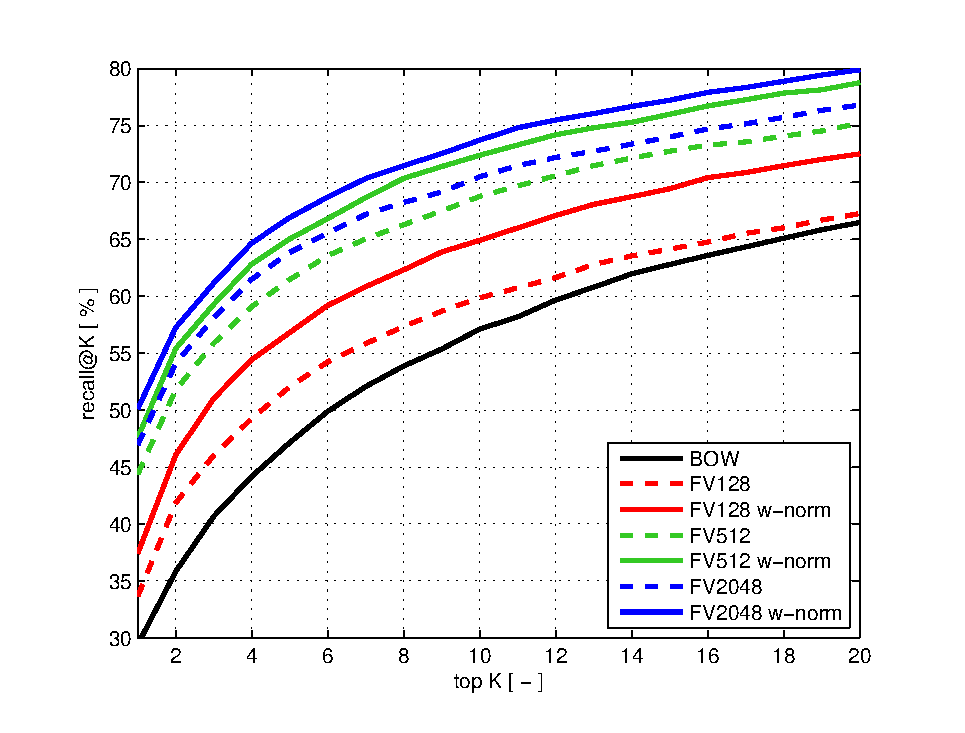
\includegraphics[width=1.1\linewidth]{imgs/plotPitt25k}  
        %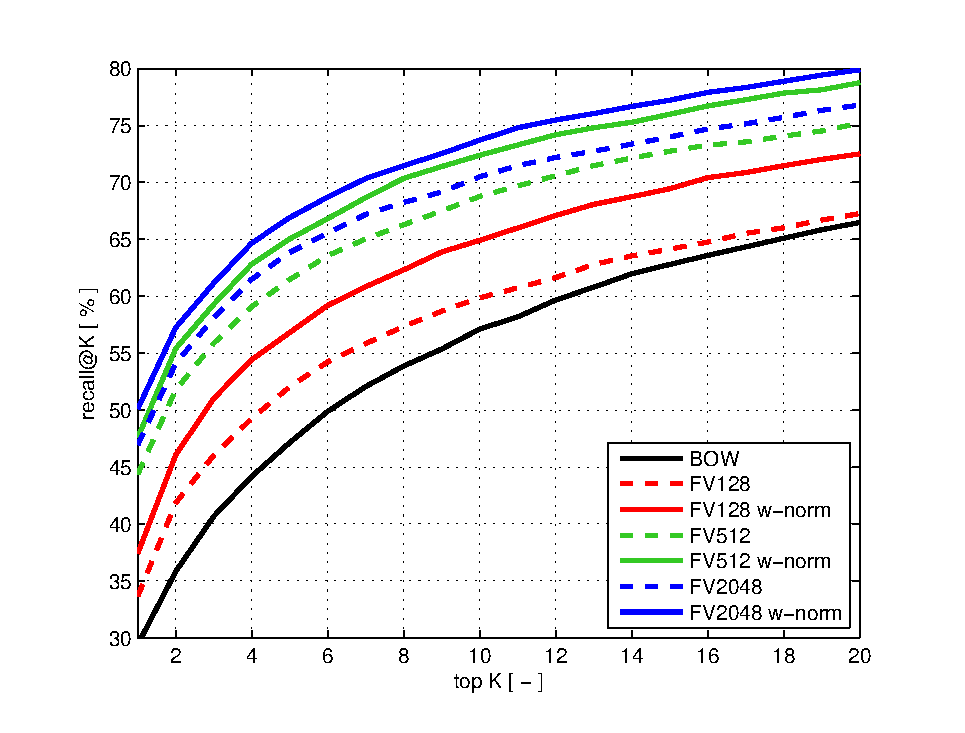
\includegraphics[trim=35mm 70mm 40mm 75mm, clip=true, width=\linewidth]{imgs/plotPitt25k}    
        \caption{
            \textbf{Evaluation on Pittsburgh 25k \cite{Gronat13} dataset for FV.} The fraction of correctly recognized queries (recall@K, y-axis) vs. the number of top $K$ retrieved database images for different Fisher vector dimensions. The learnt descriptors by the proposed method (FV w-norm) consistently improve over the raw Fisher vector descriptors across the whole range of $K$ and all dimensions.
        }
        \label{fig:recall}
    \end{figure}

  \subsection{Bag-of-words}
  As shown in table \ref{tab:recall01} both methods improve over the BOW baseline. Figure~\ref{fig:recallBOW} shows the results in a curve. Notice that while the \emph{p-val} calibration improves the recall for small values of $K$ the \emph{w-norm} method improves the recall for larger short lists. This is related to the fact that the calibration from the the negative data has the advantage that the precision is privileged over recall as discussed in Section \ref{sec:calibration}.
  

    \begin{figure}[t!]
        \centering
        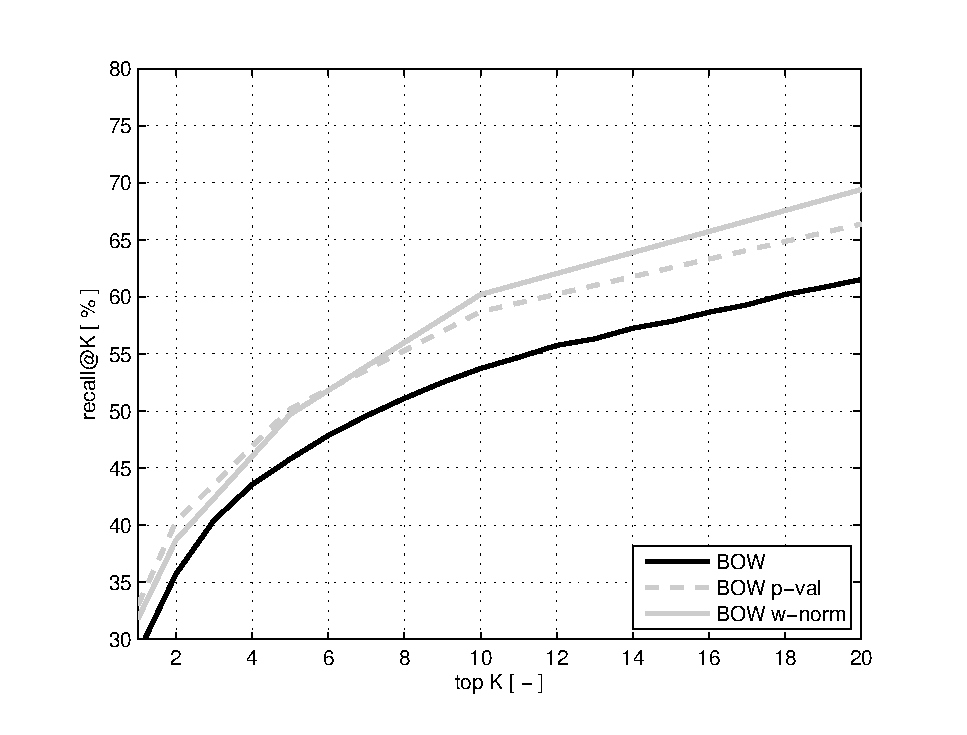
\includegraphics[width=1.1\linewidth]{imgs/plotPitt25kBOW}  
        %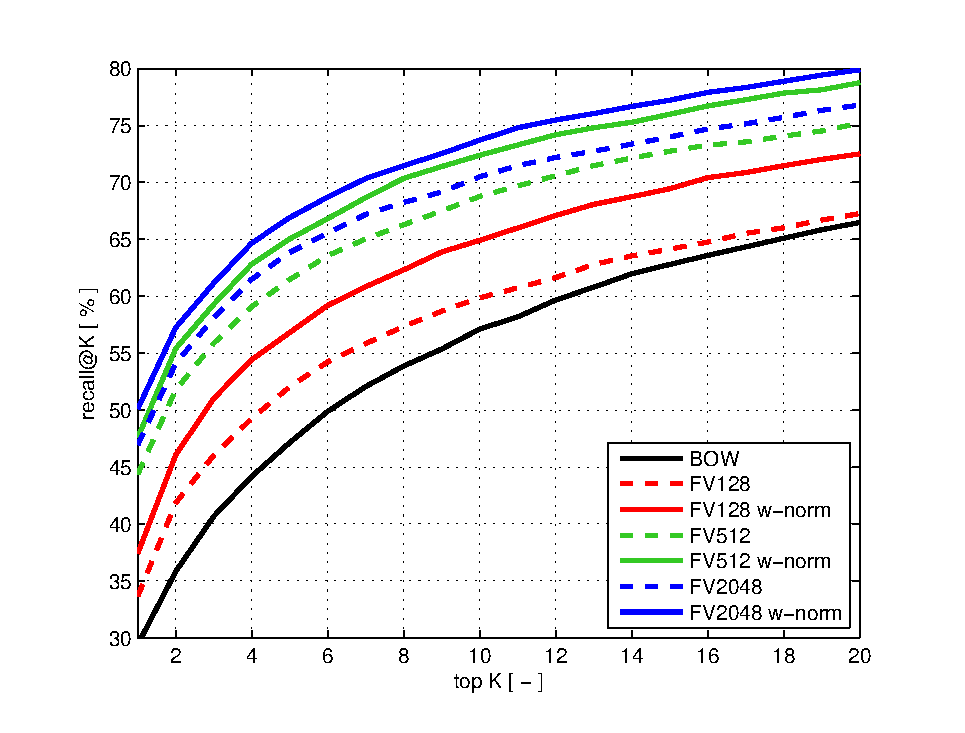
\includegraphics[trim=35mm 70mm 40mm 75mm, clip=true, width=\linewidth]{imgs/plotPitt25k}    
        \caption{
            \textbf{Evaluation on Pittsburgh 25k \cite{Gronat13} dataset for BOW.} The fraction of correctly recognized queries (recall@K, y-axis) vs. the number of top $K$ retrieved database images for different calibration methods.
        }
        \label{fig:recallBOW}
    \end{figure}

  % \paragraph{Comparison to other methods.}
  %   On the Pittsburgh 25k database, we compare performance of our learnt discriminative descriptors to the methods of~\cite{Gronat13} and~\cite{Knopp2010}, who report on the same testing data top $K=1$ recall of 36.5\% and 41.9\%, respectively (results taken from~\cite{Gronat13}). 
  %   Our method outperforms~\cite{Knopp2010} already for dimension $d=128$ (37.8\%) and~\cite{Gronat13} for dimension $d=512$ (47.6\%). Furthermore, note that~\cite{Gronat13,Knopp2010} are based on a bag-of-visual-words representation, which typically needs to store between 1000-2000 non-zero visual words per image, which is significantly more than our learnt 128 or 512 dimensional descriptor. 
       
  \subsection{Memory complexity analysis}
    Figure~\ref{fig:memory} compares the performance of proposed methods vs. space complexity. The results demonstrate that for a given level of accuracy (y-axis) the method learns a more compact (lower-dimensional) representation (x-axis). 
    For example, our learnt 128-dimensional descriptor which space complexit for Pittsburgh 25k dataset is 24MB achieves a similar accuracy, around 65\%, to the 256-dimensional raw Fisher descriptor whit memory complexity of 51MB. The \emph{w-norm} essentially reduces the memory complexity to 50\% for the same level of performance. Note that similar to~\cite{Jegou12}, we observe decrease in performance at high-dimensions for both the baseline and our method. The figure also demonstrates the advantage of usage of compressed Fisher vector representation over the BOW in terms of memory efficiency.  

    \begin{figure}[t!]
        \centering
        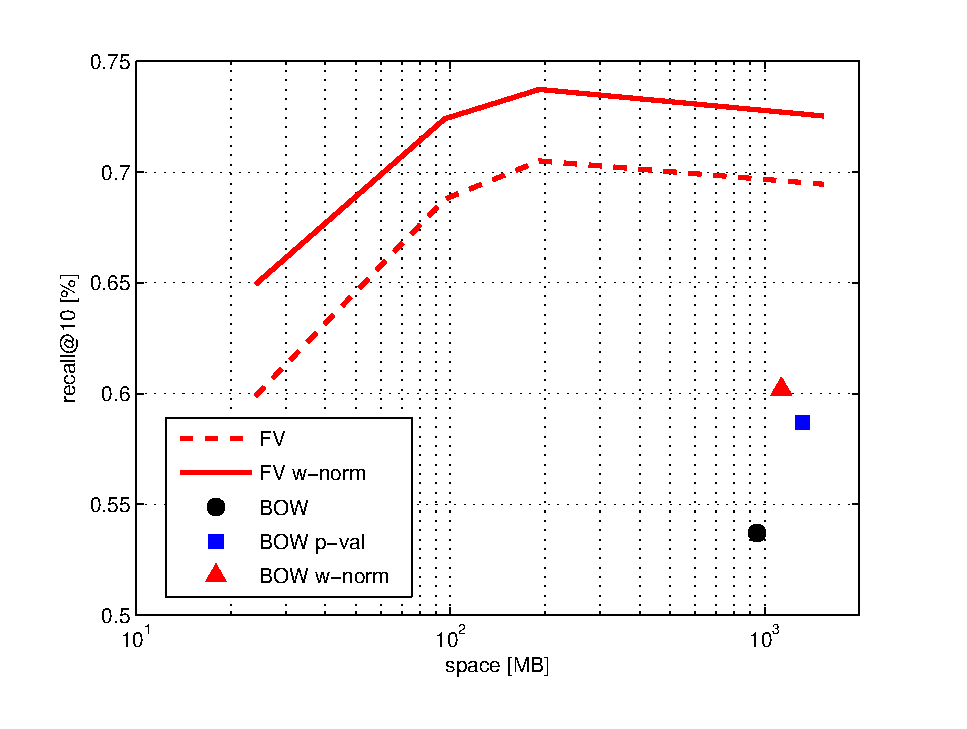
\includegraphics[width=1.1\linewidth]{imgs/FVmemory02}    
        \caption{
            \textbf{Memory complexity analysis for Pittsburgh 25k dataset.} 
            The fraction of correctly localized queries at the top 10 retrieved images (y-axis) vs. memory complexity (x-axis) for different methods. The learnt descriptors by the FV \emph{w renorm} mehtod clearly outperform the raw Fisher vector descriptors (FV) in terms of memory efficiency. Note that for a certain level of performance (y-axis) the proposed method learns a more memory efficient (lower dimensional) descriptor.
        }
        \label{fig:memory}
    \end{figure}

  \subsection{Visualizations}
    \begin{table}[t!]
\begin{centering}
	\begin{tabularx}{0.89\linewidth}{|l|c c c c c|}
		\hline 
		\rowcolor{maroon!50}
		Method: & \multicolumn{5}{c|}{55k Pittsburgh} \\
		\hline 
		\hline 
		%%%%%%%%%%%%%%%%%%%%%%%%%%%%%%%%%%%%%%%%%%%%%%%%%%%%%%%%%%%%%%%%%%%%%%%%%%%%
		\rowcolor{maroon!50}
		recall@K [$\%$] & 1 & 2 & 5 & 10 & 20\\
		\hline
		\rowcolor{maroon!10}
		BOW       & 8.7 & 11.0 & 17.3 & 22.8 & 25.4  \\
    \hline
    %%%%%%%%%%%%%%%%%%%%%%%%%%%%%%%%%%%%%%%%%%%%%%%%%%%%%%%%%%%%%%%%%%%%%%%%%%%%
		\rowcolor{maroon!10}
		FV128     & 10.9 & 14.1 & 20.2 & 26.4 & 33.2 \\
		\rowcolor{maroon!10}
		\textbf{FV128 w renorm}  & \textbf{13.5}  &  \textbf{17.7}  &  \textbf{25.0}  &  \textbf{31.8}  &  \textbf{39.0} \\
    \hline  
    %%%%%%%%%%%%%%%%%%%%%%%%%%%%%%%%%%%%%%%%%%%%%%%%%%%%%%%%%%%%%%%%%%%%%%%%%%%%%
    \rowcolor{maroon!10}
    FV512   & 17.3 &  21.1 &  28.4 &  34.2 &  40.3 \\      
    \rowcolor{maroon!10}
    % FV512 p-val   & \textbf{}  & \textbf{} & \textbf{} & \textbf{} & \textbf{}  &
    %                          \textbf{} &  \textbf{} &  \textbf{}  & \textbf{} &  \textbf{} \\
    \rowcolor{maroon!10}
    \textbf{FV512 w renorm}  & \textbf{19.8} &  \textbf{25.1} &  \textbf{32.7}  & \textbf{38.7} &  \textbf{46.0} \\
    \hline
    %%%%%%%%%%%%%%%%%%%%%%%%%%%%%%%%%%%%%%%%%%%%%%%%%%%%%%%%%%%%%%%%%%%%%%%%%%%%%%
		\rowcolor{maroon!10}
		FV2048        & 19.2 & 23.5 & 29.9 &  35.2 &  41.9 \\
		\rowcolor{maroon!10}
		% FV2048 p-val  & \textbf{} & \textbf{} & \textbf{} & \textbf{} & \textbf{} &
  %       \textbf{} & \textbf{} & \textbf{} & \textbf{} & \textbf{}\\
        \rowcolor{maroon!10}
        \textbf{FV2048 w renorm}  & \textbf{20.8} & \textbf{25.9} & \textbf{33.1} & \textbf{38.7} & \textbf{45.9} \\
        \hline
        %%%%%%%%%%%%%%%%%%%%%%%%%%%%%%%%%%%%%%%%%%%%%%%%%%%%%%%%%%%%%%%%%%%%%%%%%%%%%%%%
  %       \rowcolor{maroon!10}
  %       FV8192        & 46.0  & 52.7 & 62.5 & 69.4 & 76.4 & - & - & - & - &  -   \\
  %       \rowcolor{maroon!10}
  %       \textbf{FV8192 w renorm}  & \textbf{48.4} & \textbf{55.6} & \textbf{65.4} & \textbf{72.6} & \textbf{79.0} & - & - & - & - & -\\
		% \hline
	\end{tabularx}
	\caption{ \textcolor{myRed}{}
%		The percentage of correctly localized test queries for which the topK ranked database image is within $20$ meters from the ground truth query position. The proposed method (svmFV) outperforms the baseline methods.
The fraction of correctly recognized queries (recall@K) vs. the number of top $K\in\{1,2,5,10,20\}$ retrieved database images for different Fisher vector dimensions $d\in\{128,512,2048\}$. The learnt descriptors by the proposed method (FV w renorm) consistently improve over the raw Fisher vector descriptors across the whole range of $K$ and all dimensions on 55k Pittsburgh image datasets.		
}
\label{tab:recall02}
\end{centering}
\end{table}

    %%%%%%%%%%% Example 1 %%%%%%%%%%%%%%%
\begin{minipage}{1.0\linewidth}
\end{minipage}
% QUERY image
\begin{minipage}{0.34\linewidth}
    \centering
    \vspace{5mm}
    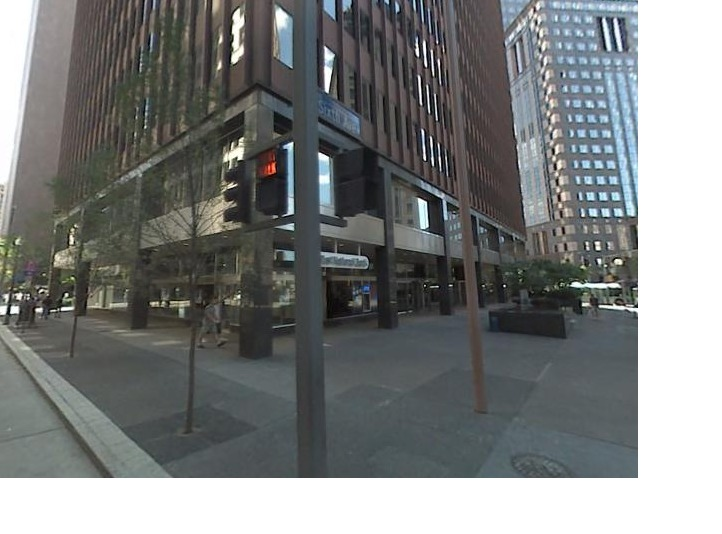
\includegraphics[height=40mm]{imgs/ex1/query.jpg}
\end{minipage}
% Retrieved images
\begin{minipage}{0.75\linewidth}
    % FV e-SVM
    \begin{minipage}{\linewidth} 
        \colorbox{myGreen}{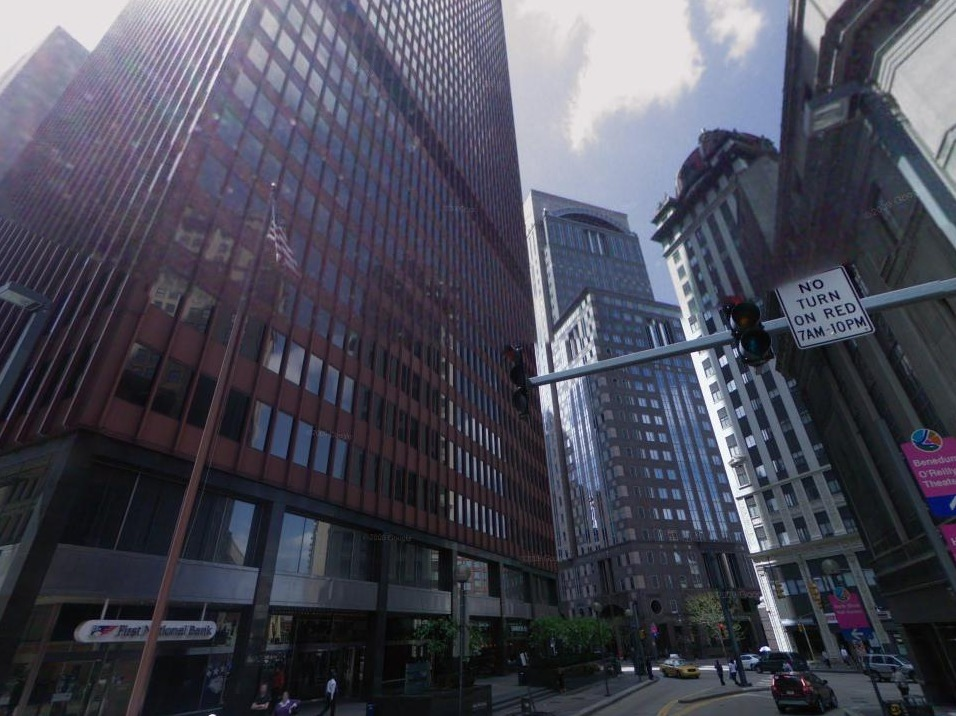
\includegraphics[height=16mm]{imgs/ex1/FVsvm1.jpg}}
        \colorbox{myGreen}{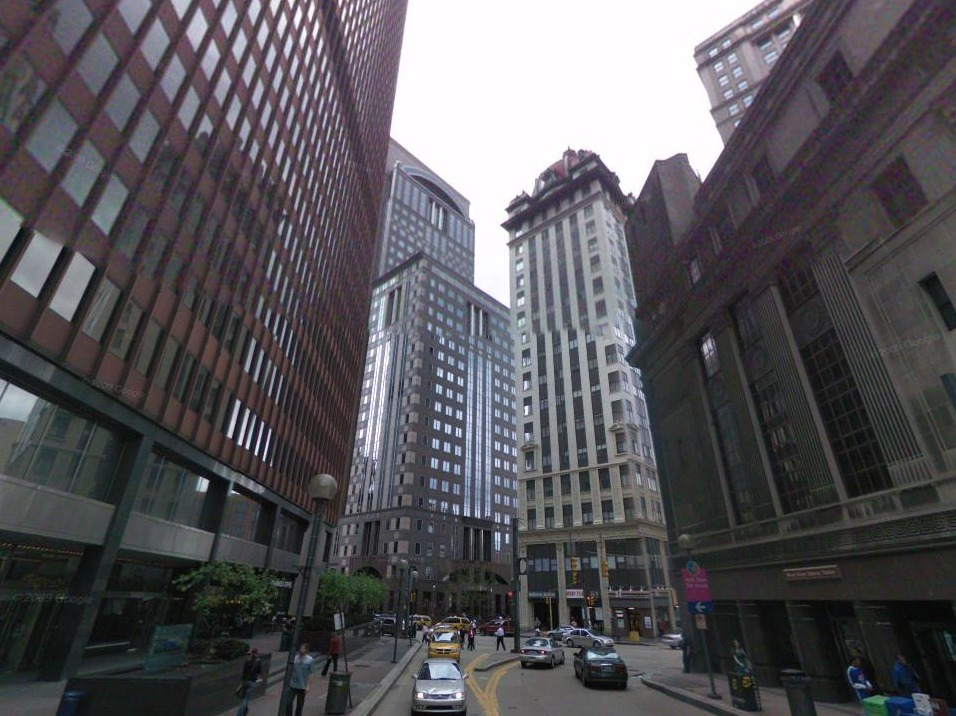
\includegraphics[height=16mm]{imgs/ex1/FVsvm2.jpg}}
        \colorbox{myGreen}{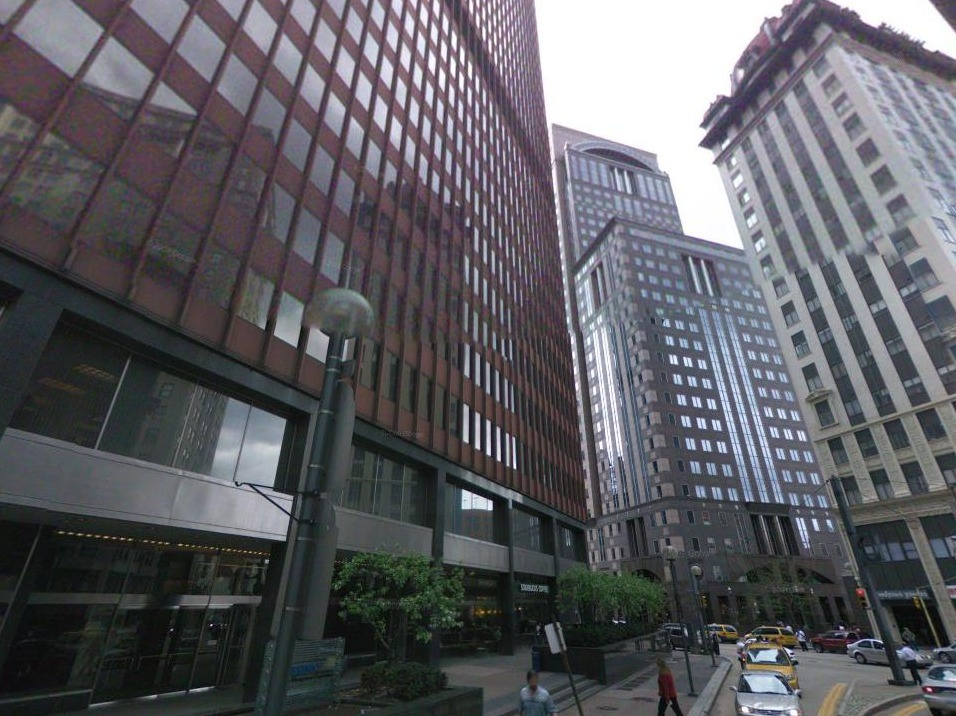
\includegraphics[height=16mm]{imgs/ex1/FVsvm3.jpg}}
        \colorbox{myGreen}{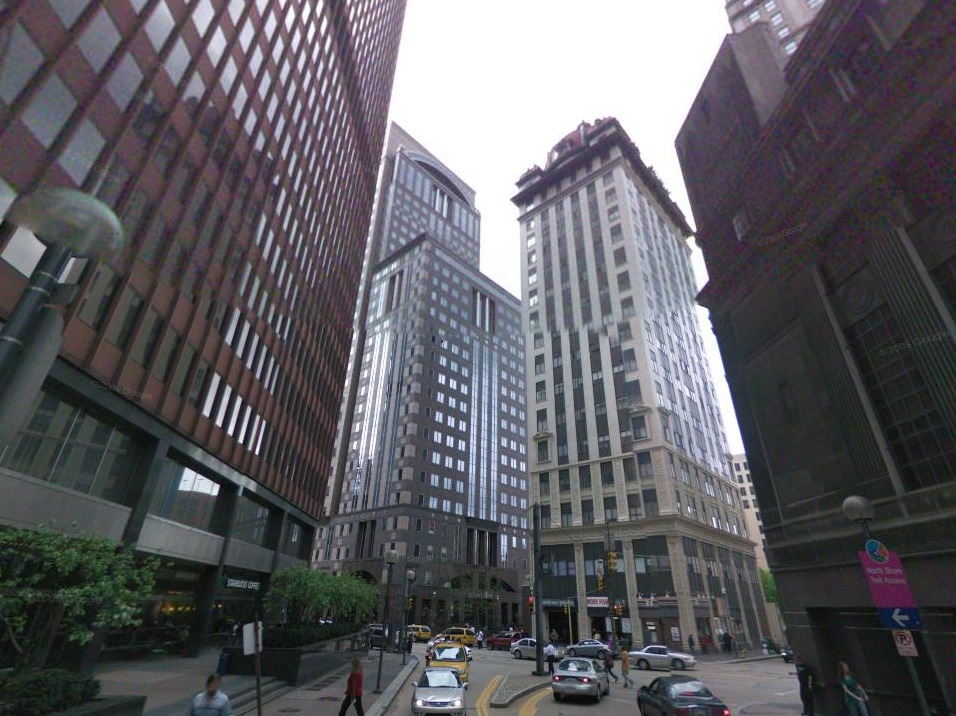
\includegraphics[height=16mm]{imgs/ex1/FVsvm4.jpg}}
    \end{minipage}
    \\
    \begin{minipage}{\linewidth}
        \colorbox{myRed}{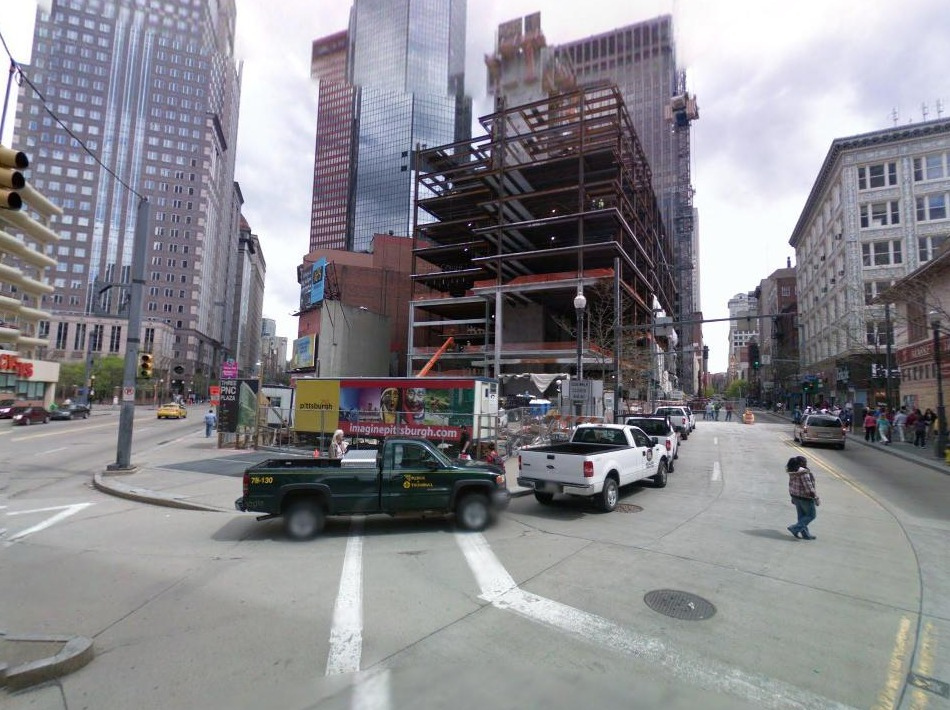
\includegraphics[height=16mm]{imgs/ex1/FV1.jpg}}
        \colorbox{myRed}{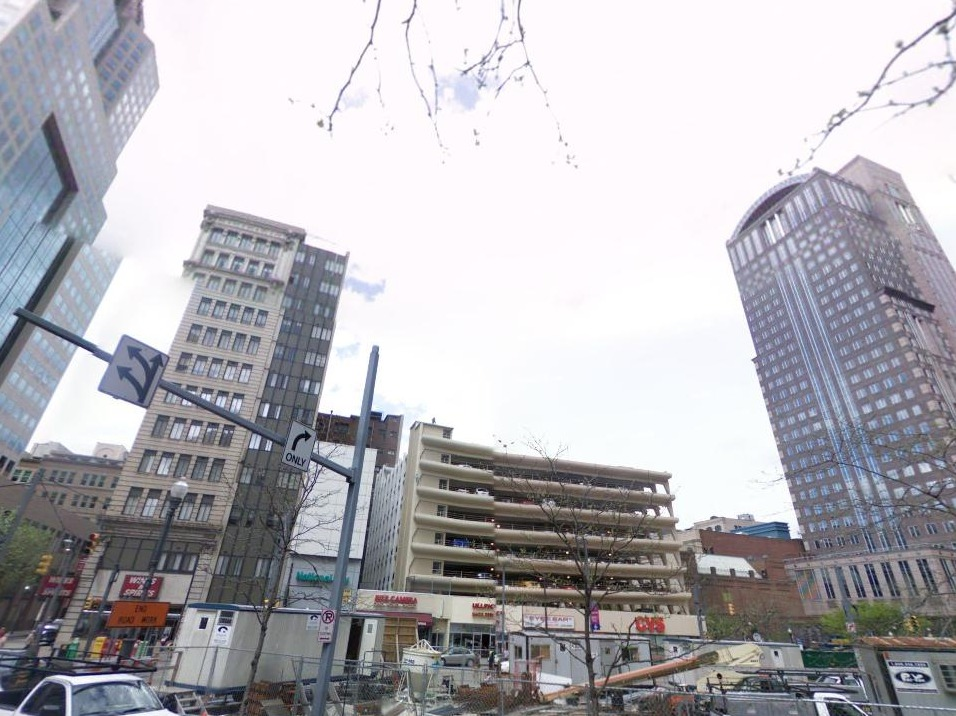
\includegraphics[height=16mm]{imgs/ex1/FV2.jpg}}
        \colorbox{myRed}{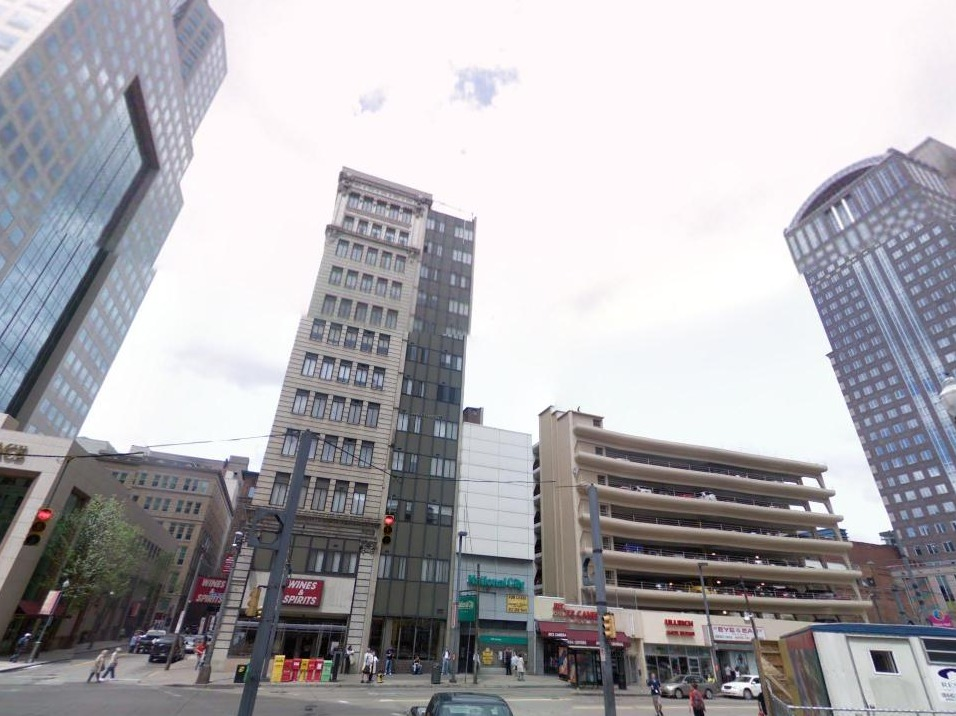
\includegraphics[height=16mm]{imgs/ex1/FV3.jpg}}
        \colorbox{myRed}{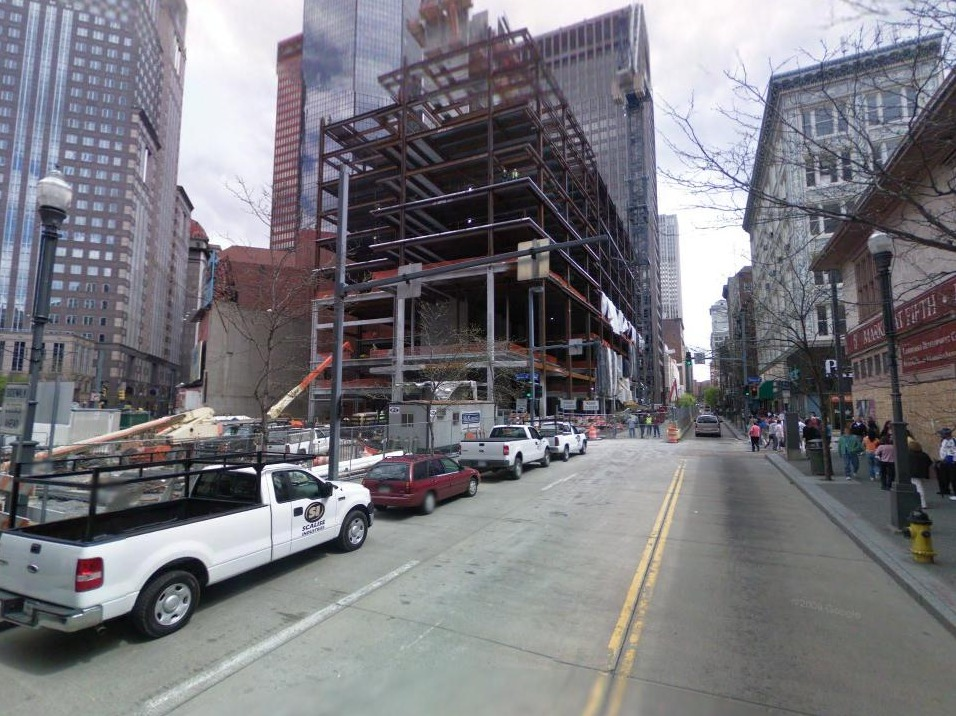
\includegraphics[height=16mm]{imgs/ex1/FV4.jpg}}
    \end{minipage} 
\end{minipage}
\\
%%%%%%%%%%% Example 2 %%%%%%%%%%%%%%%
\begin{minipage}{0.34\linewidth}
    \centering
    \vspace{0mm}
    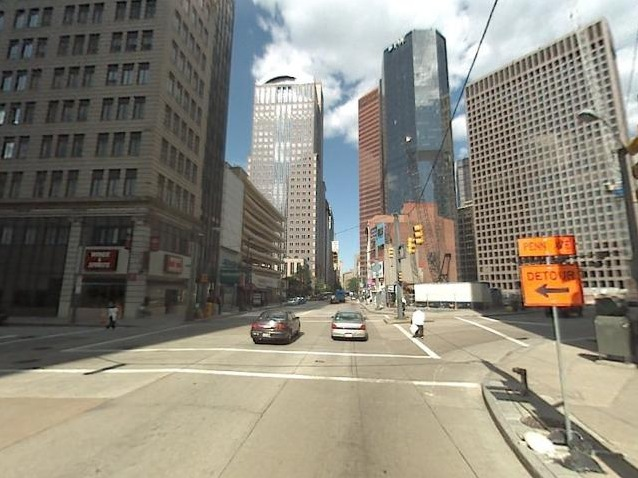
\includegraphics[height=36mm]{imgs/ex2/query.jpg}
\end{minipage}
% Retrieved images
\begin{minipage}{0.75\linewidth}
    % FV e-SVM
    \begin{minipage}{\linewidth} 
        \colorbox{myGreen}{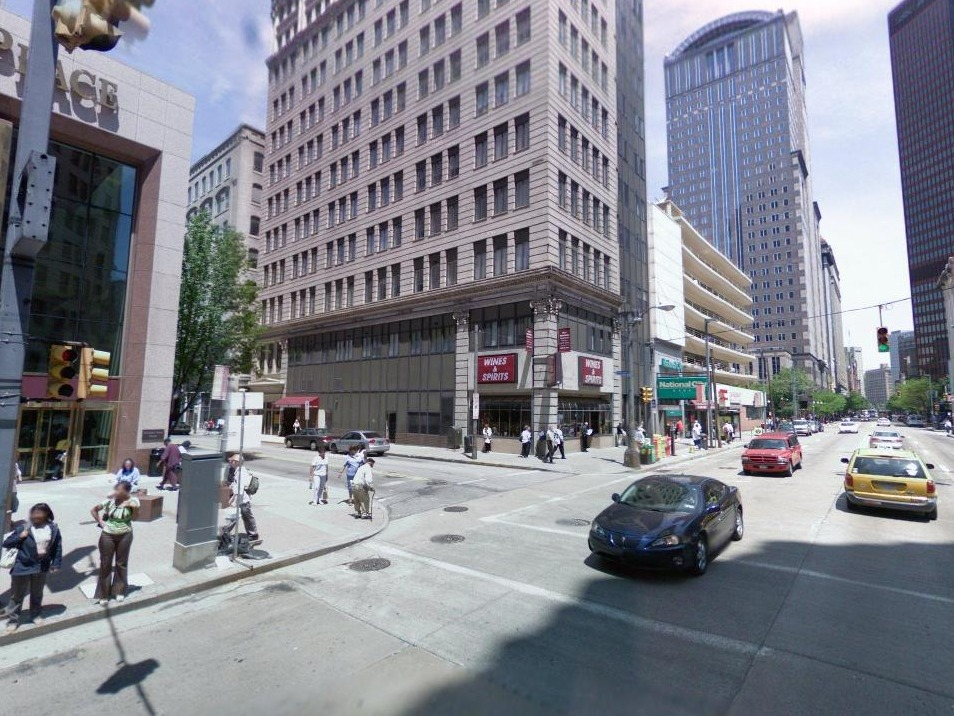
\includegraphics[height=16mm]{imgs/ex2/FVsvm1.jpg}}
        \colorbox{myGreen}{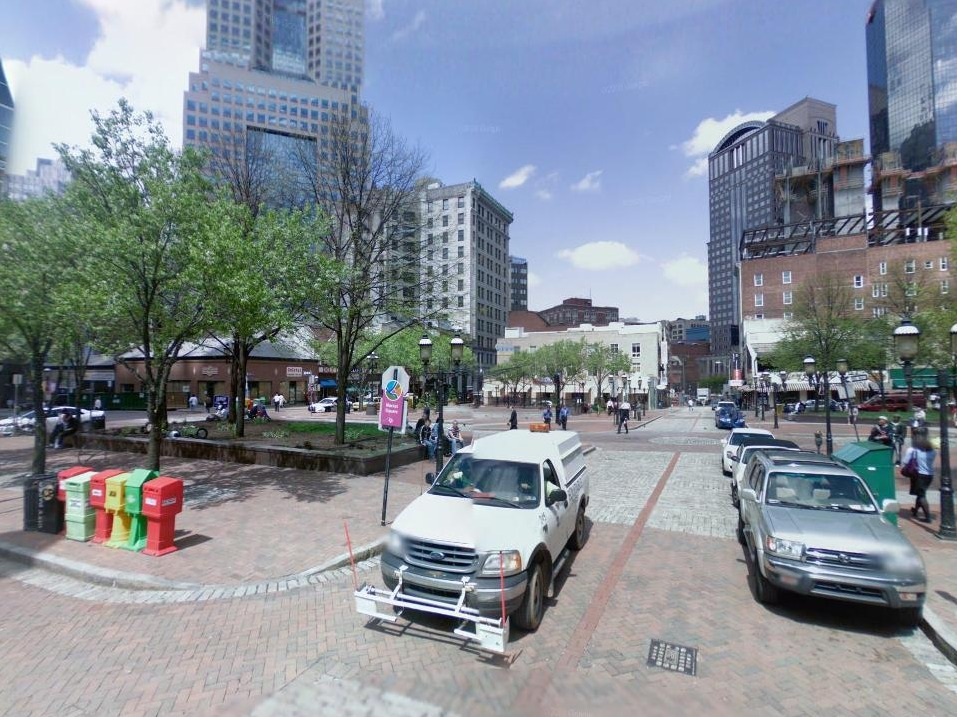
\includegraphics[height=16mm]{imgs/ex2/FVsvm2.jpg}}
        \colorbox{myGreen}{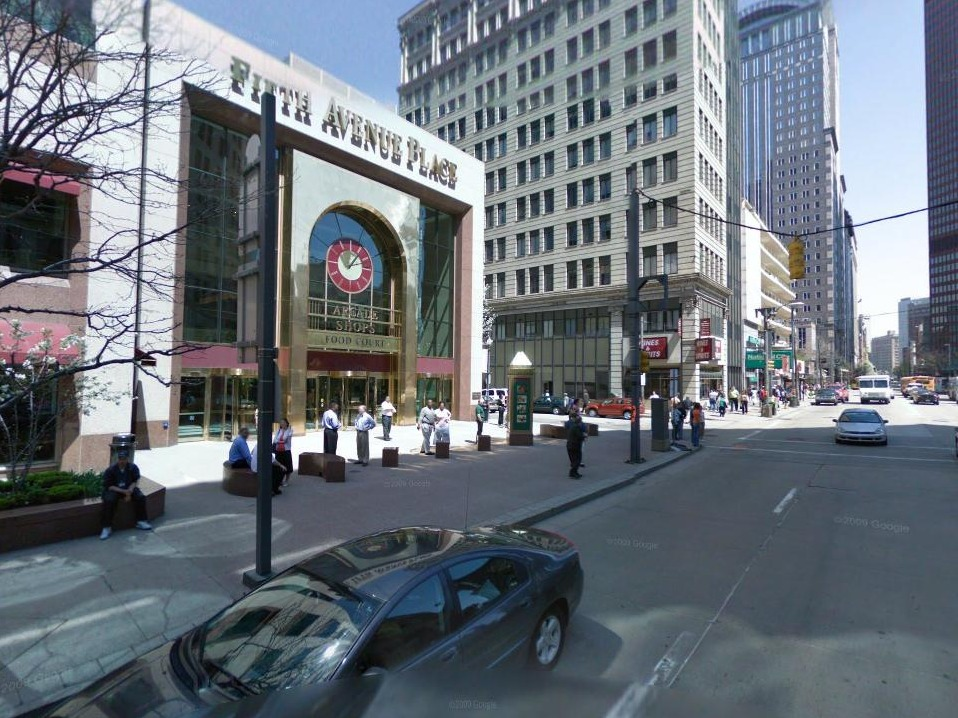
\includegraphics[height=16mm]{imgs/ex2/FVsvm3.jpg}}
        \colorbox{myGreen}{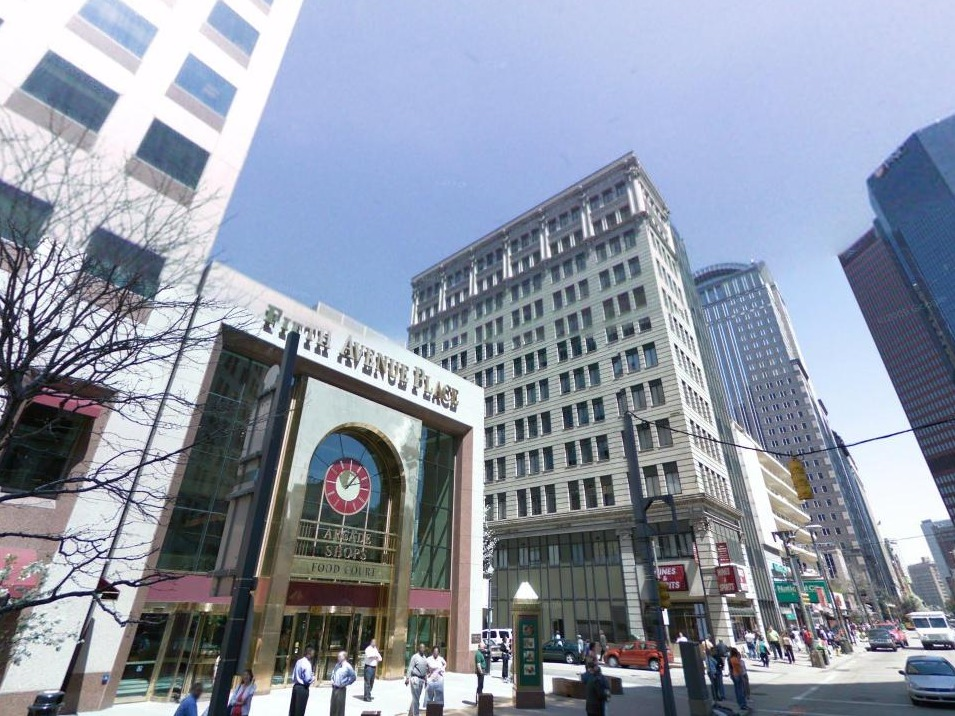
\includegraphics[height=16mm]{imgs/ex2/FVsvm4.jpg}}
    \end{minipage}
    \\
    \begin{minipage}{\linewidth}
        \colorbox{myRed}{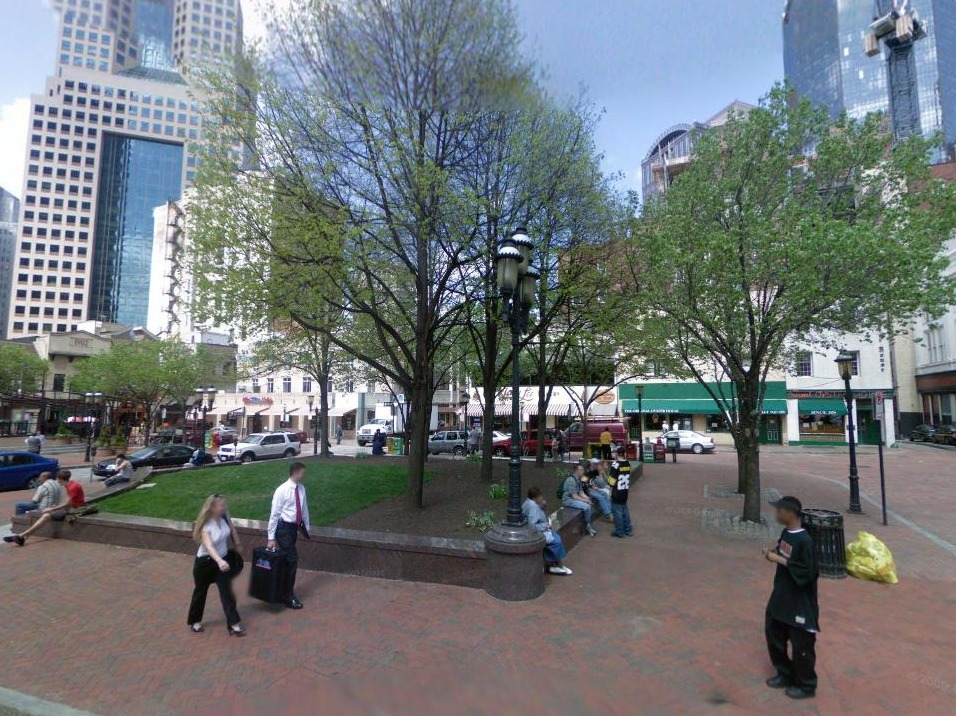
\includegraphics[height=16mm]{imgs/ex2/FV1.jpg}}
        \colorbox{myRed}{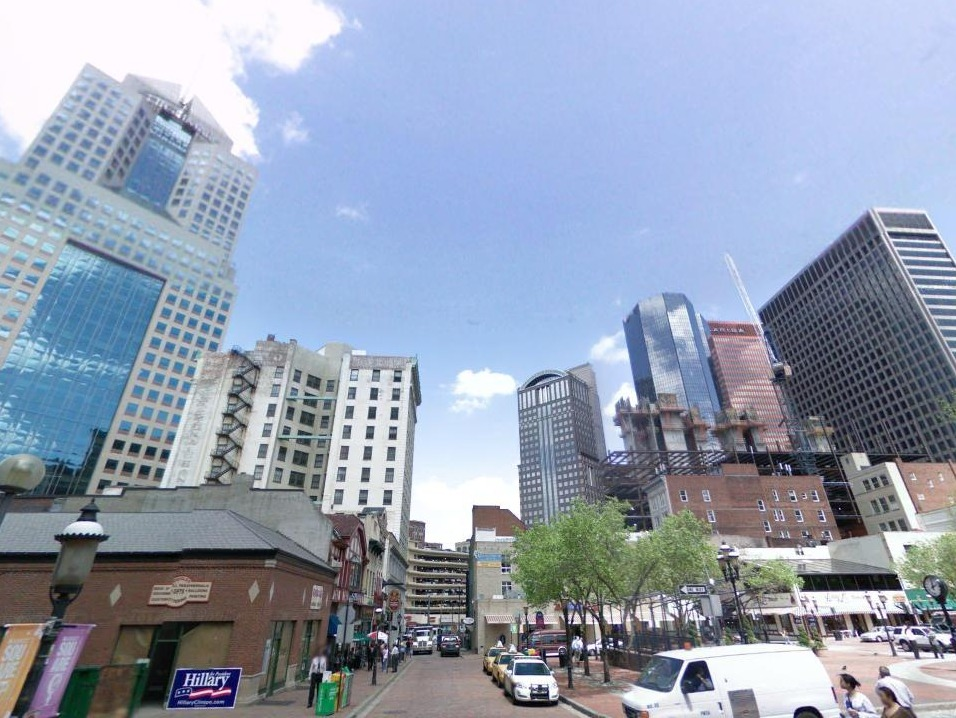
\includegraphics[height=16mm]{imgs/ex2/FV2.jpg}}
        \colorbox{myRed}{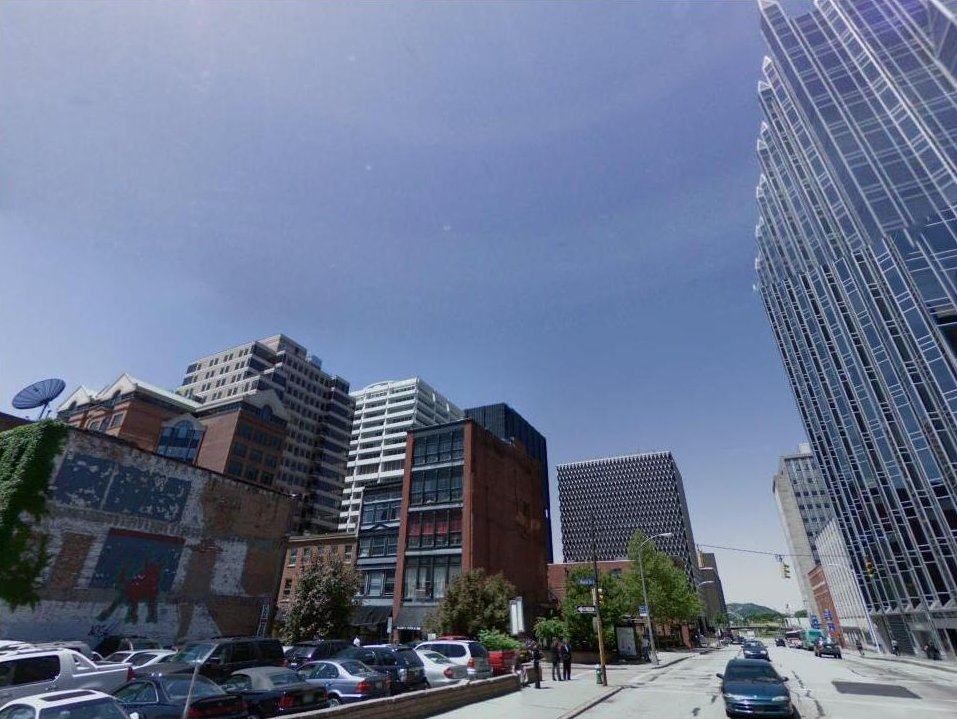
\includegraphics[height=16mm]{imgs/ex2/FV3.jpg}}
        \colorbox{myRed}{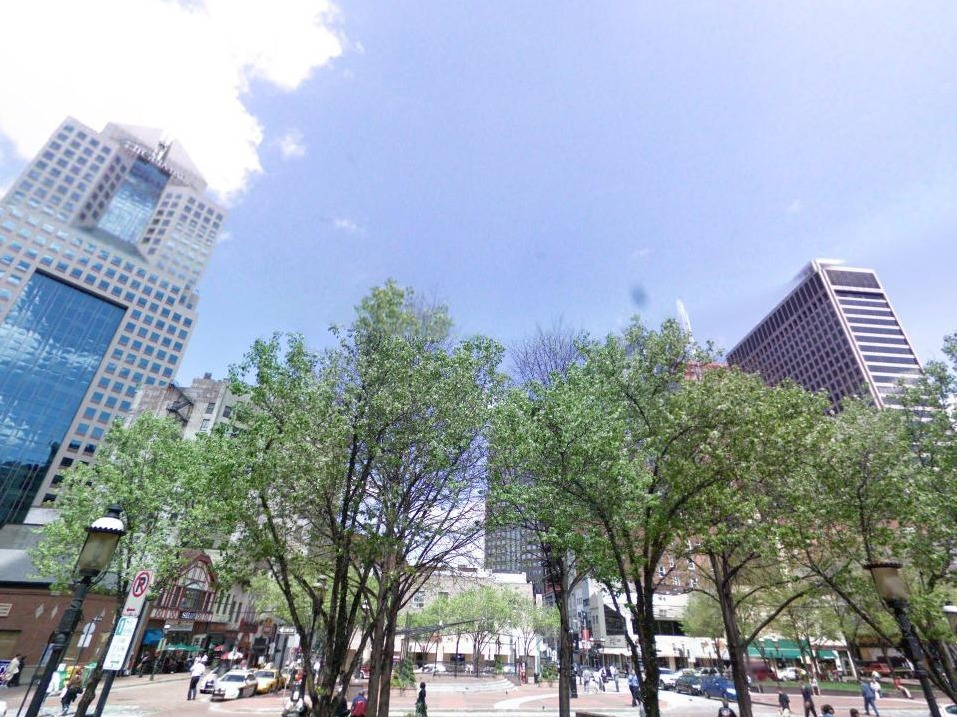
\includegraphics[height=16mm]{imgs/ex2/FV4.jpg}}
    \end{minipage} 
\end{minipage}
\vspace{3mm}
\\
%%%%%%%%%%% Example 3 %%%%%%%%%%%%%%%
\begin{minipage}{0.34\linewidth}
    \centering
    \vspace{0mm}
    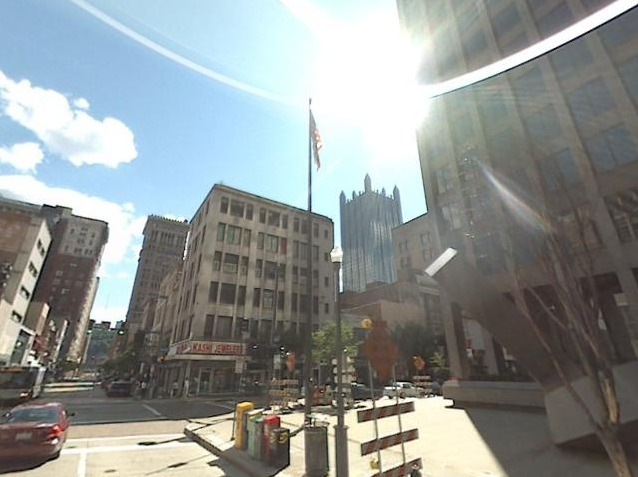
\includegraphics[height=36mm]{imgs/ex3/query.jpg}
\end{minipage}
% Retrieved images
\begin{minipage}{0.75\linewidth}
    % FV e-SVM
    \begin{minipage}{\linewidth} 
        \colorbox{myGreen}{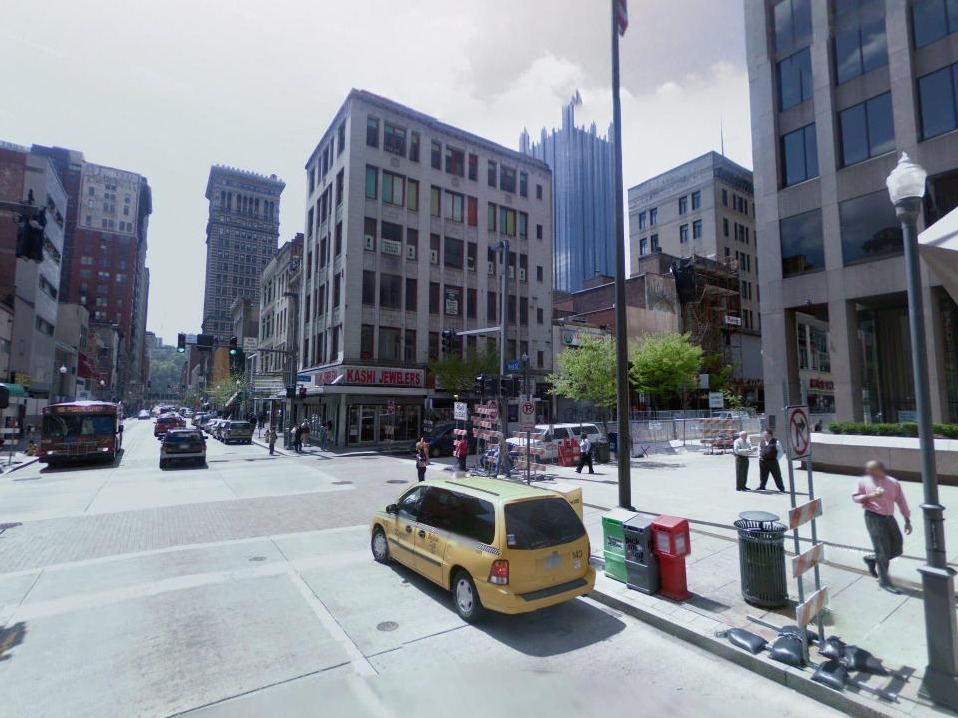
\includegraphics[height=16mm]{imgs/ex3/FVsvm1.jpg}}
        \colorbox{myRed}{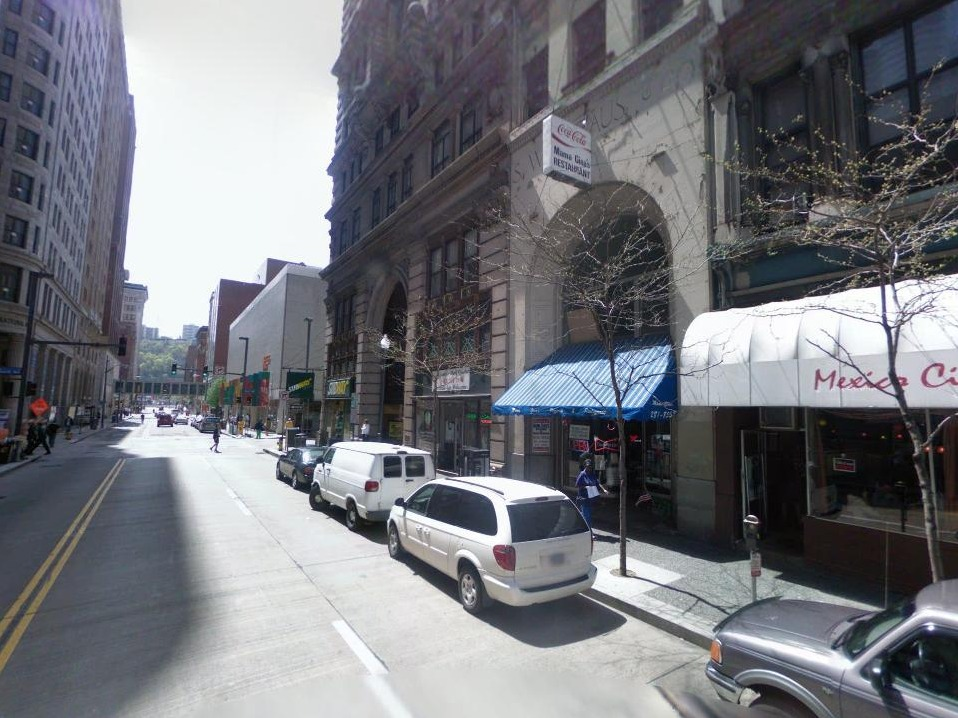
\includegraphics[height=16mm]{imgs/ex3/FVsvm2.jpg}}
        \colorbox{myGreen}{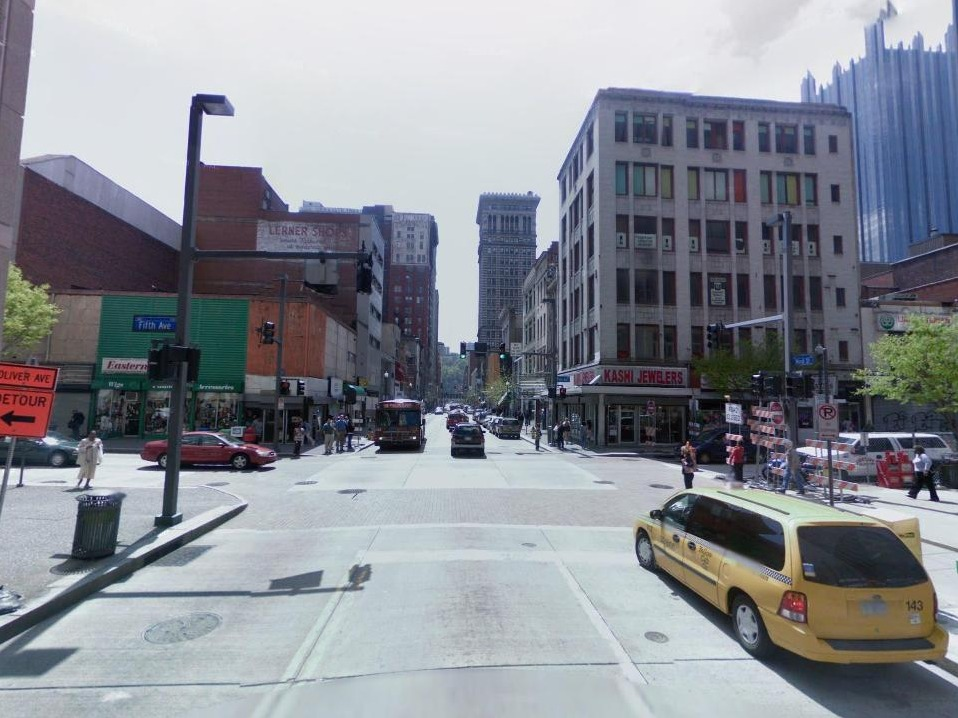
\includegraphics[height=16mm]{imgs/ex3/FVsvm5.jpg}}
        \colorbox{myGreen}{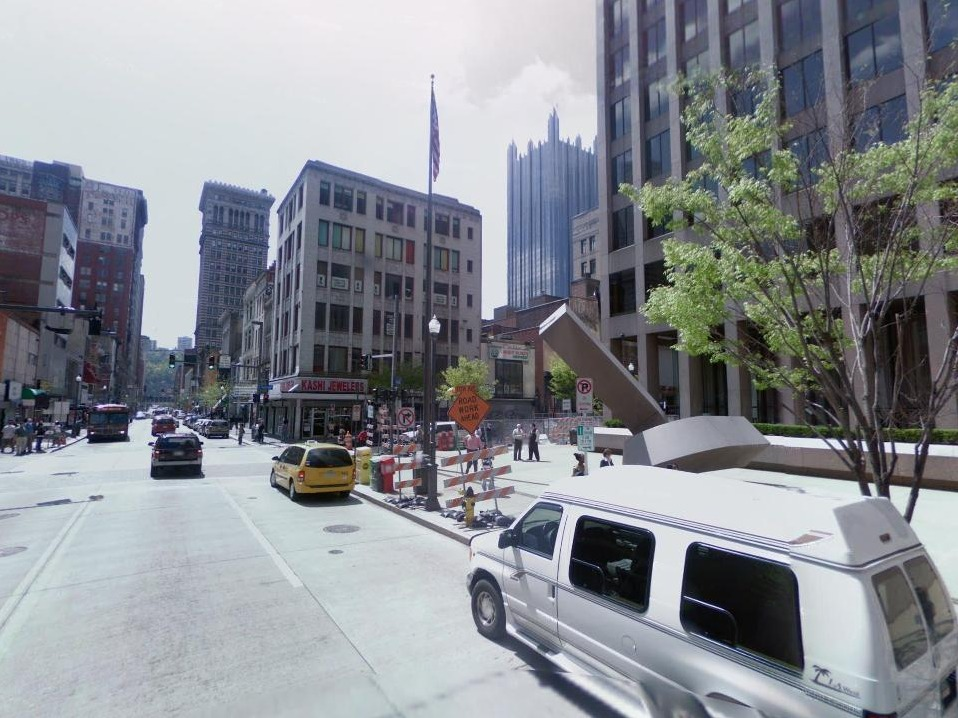
\includegraphics[height=16mm]{imgs/ex3/FVsvm4.jpg}}
    \end{minipage}
    \\
    \begin{minipage}{\linewidth}
        \colorbox{myRed}{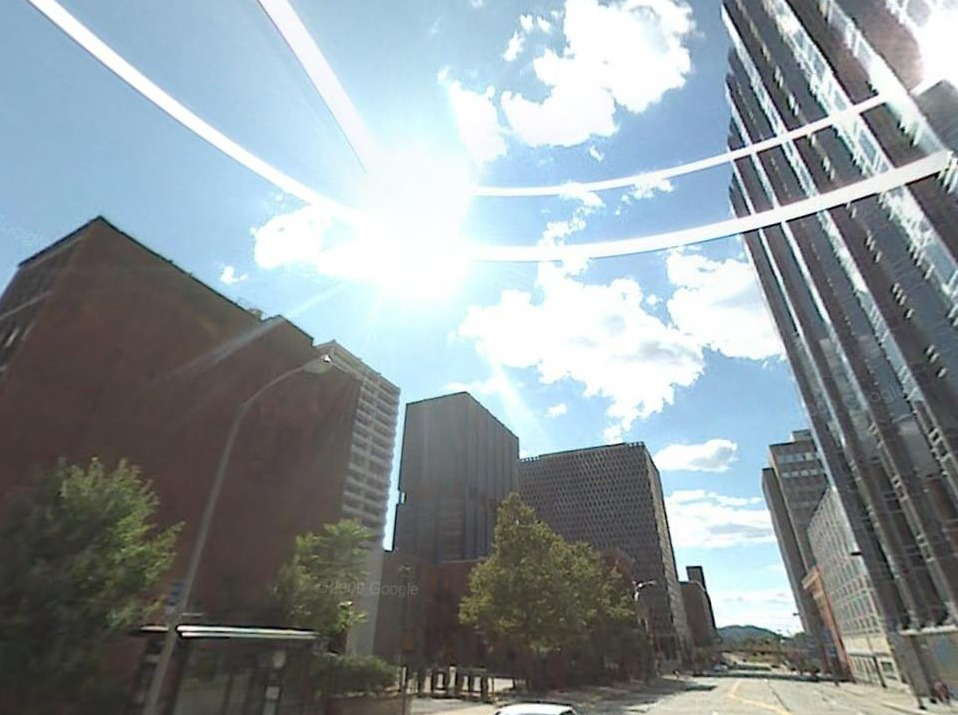
\includegraphics[height=16mm]{imgs/ex3/FV1.jpg}}
        \colorbox{myGreen}{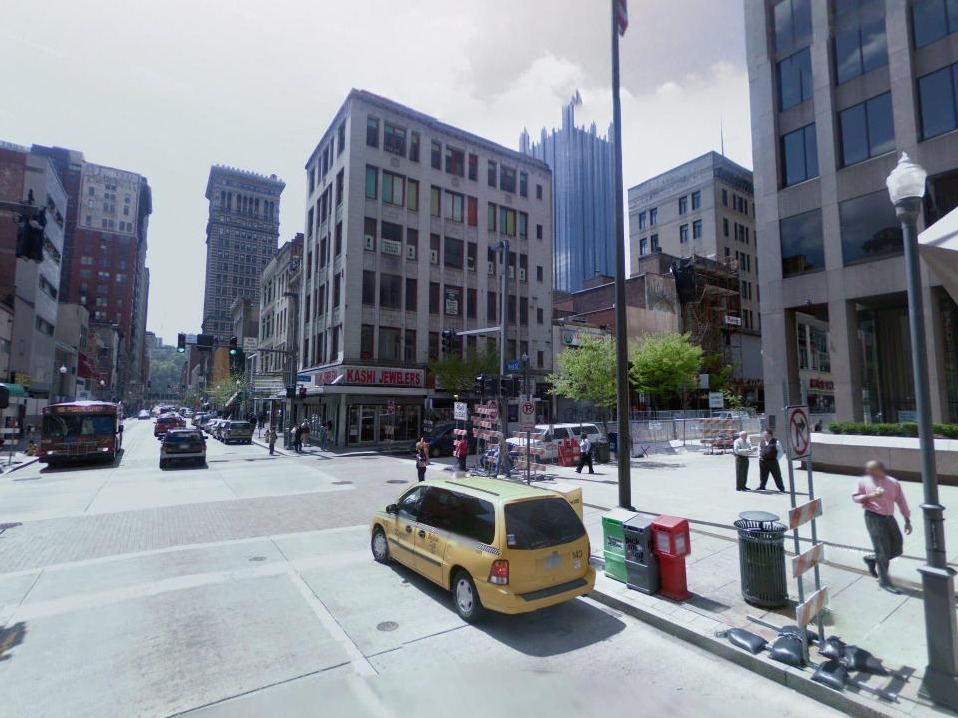
\includegraphics[height=16mm]{imgs/ex3/FV2.jpg}}
        \colorbox{myRed}{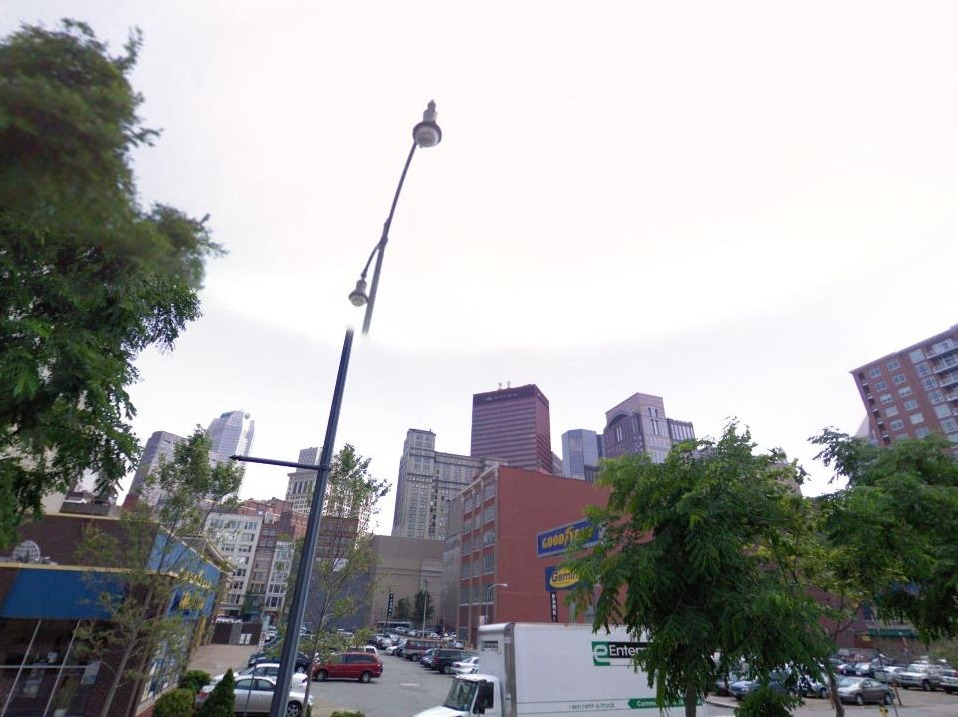
\includegraphics[height=16mm]{imgs/ex3/FV3.jpg}}
        \colorbox{myRed}{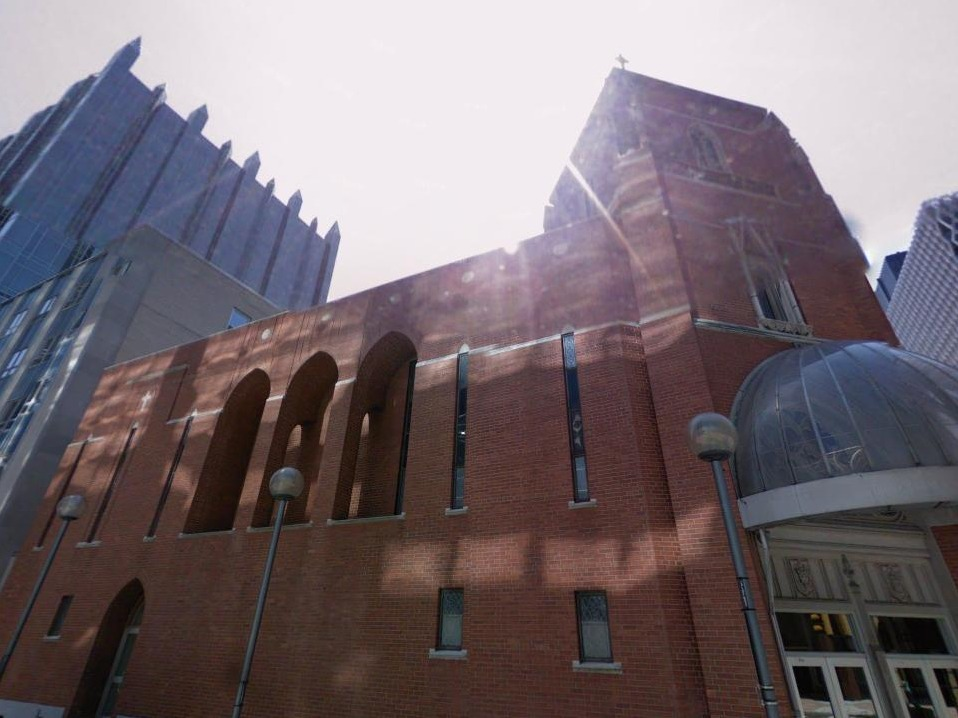
\includegraphics[height=16mm]{imgs/ex3/FV4.jpg}}
    \end{minipage} 
\end{minipage}
\vspace{3mm}
\\
%%%%%%%%%%% Example 4 %%%%%%%%%%%%%%%
\begin{minipage}{0.34\linewidth}
    \centering
    \vspace{0mm}
    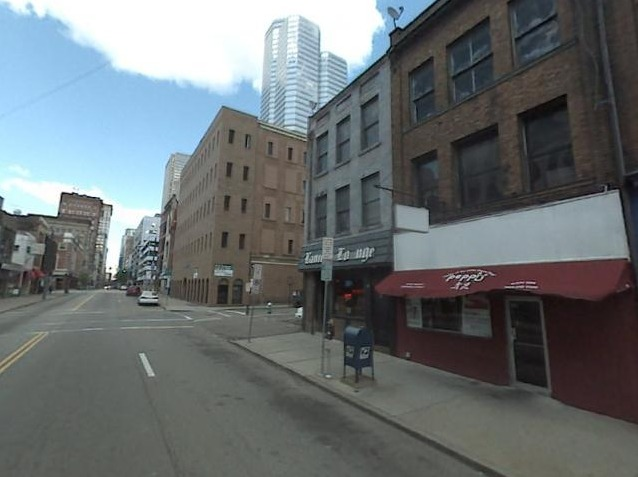
\includegraphics[height=36mm]{imgs/ex4/query.jpg}
\end{minipage}
% Retrieved images
\begin{minipage}{0.75\linewidth}
    % FV e-SVM
    \begin{minipage}{\linewidth} 
        \colorbox{myGreen}{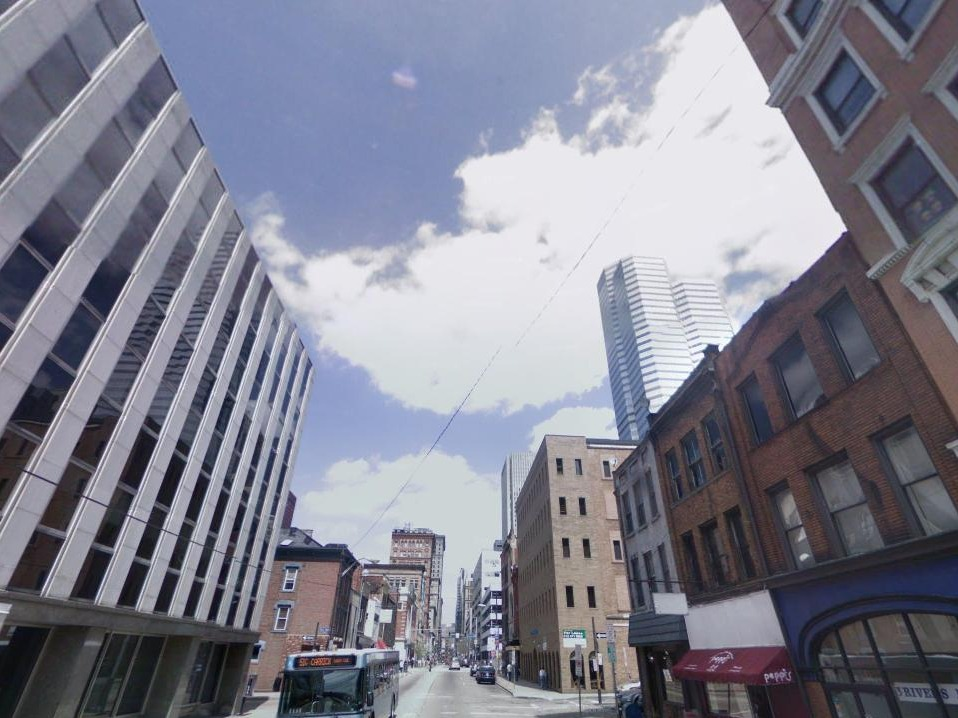
\includegraphics[height=16mm]{imgs/ex4/FVsvm1.jpg}}
        \colorbox{myRed}{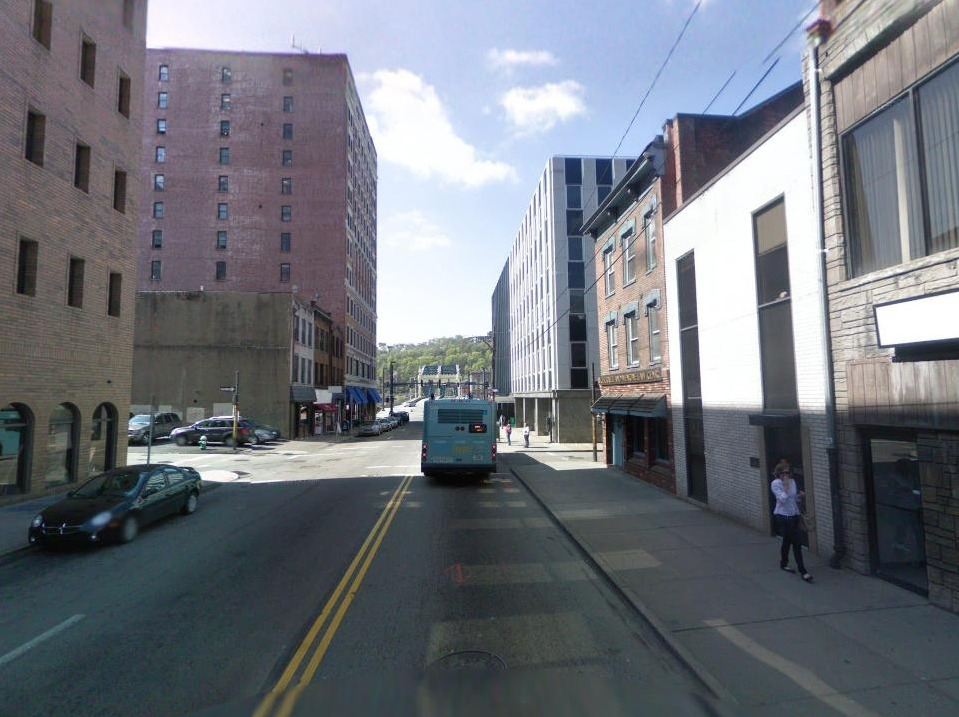
\includegraphics[height=16mm]{imgs/ex4/FVsvm2.jpg}}
        \colorbox{myGreen}{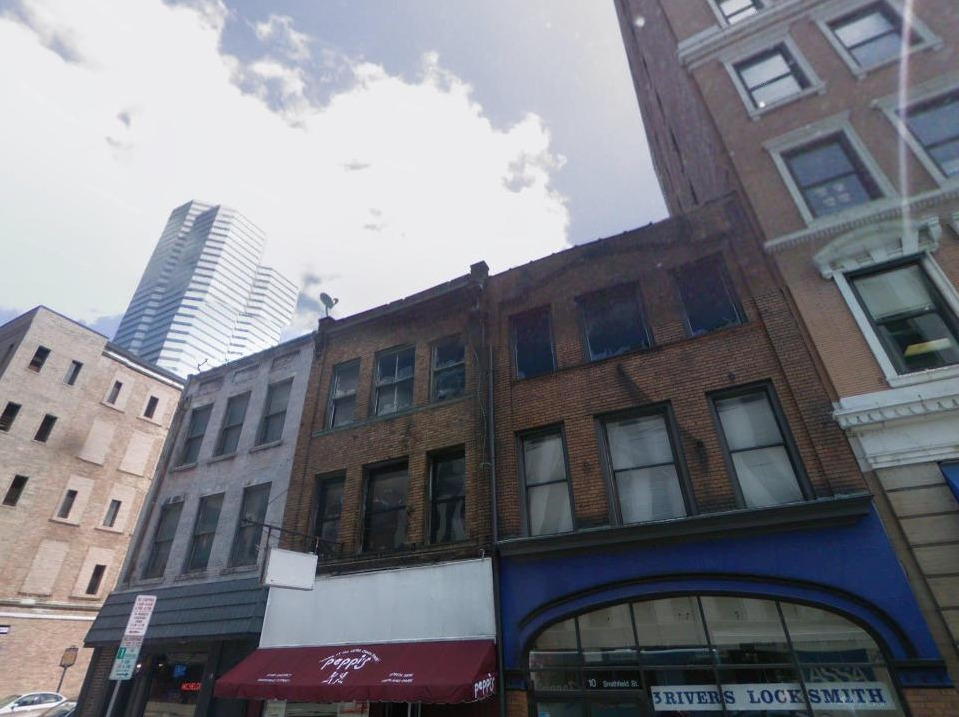
\includegraphics[height=16mm]{imgs/ex4/FVsvm5.jpg}}
        \colorbox{myGreen}{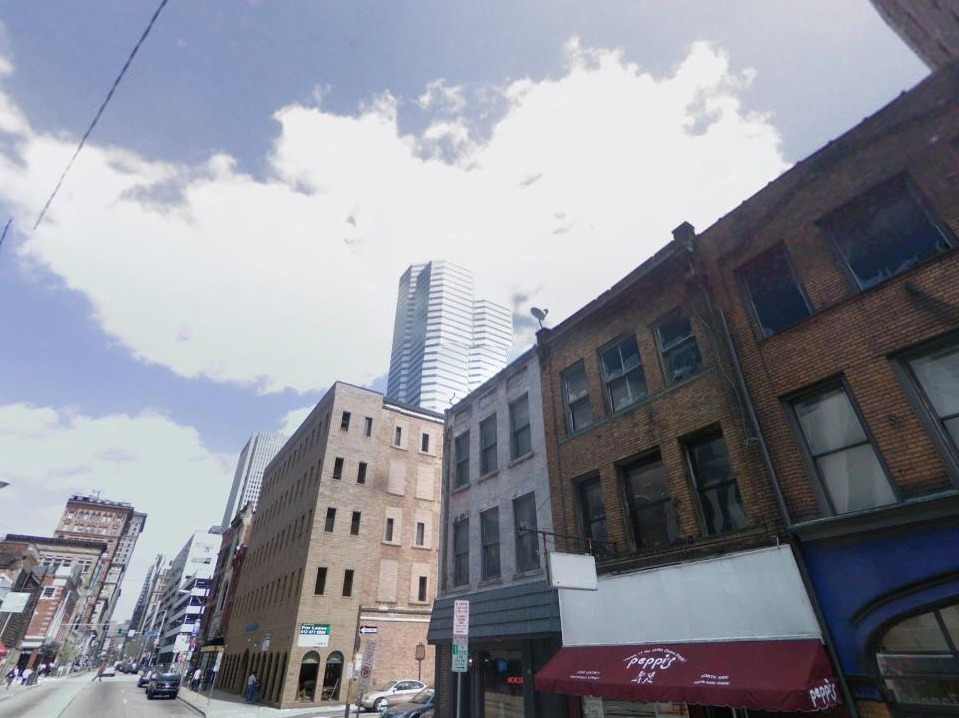
\includegraphics[height=16mm]{imgs/ex4/FVsvm4.jpg}}
    \end{minipage}
    \\
    \begin{minipage}{\linewidth}
        \colorbox{myRed}{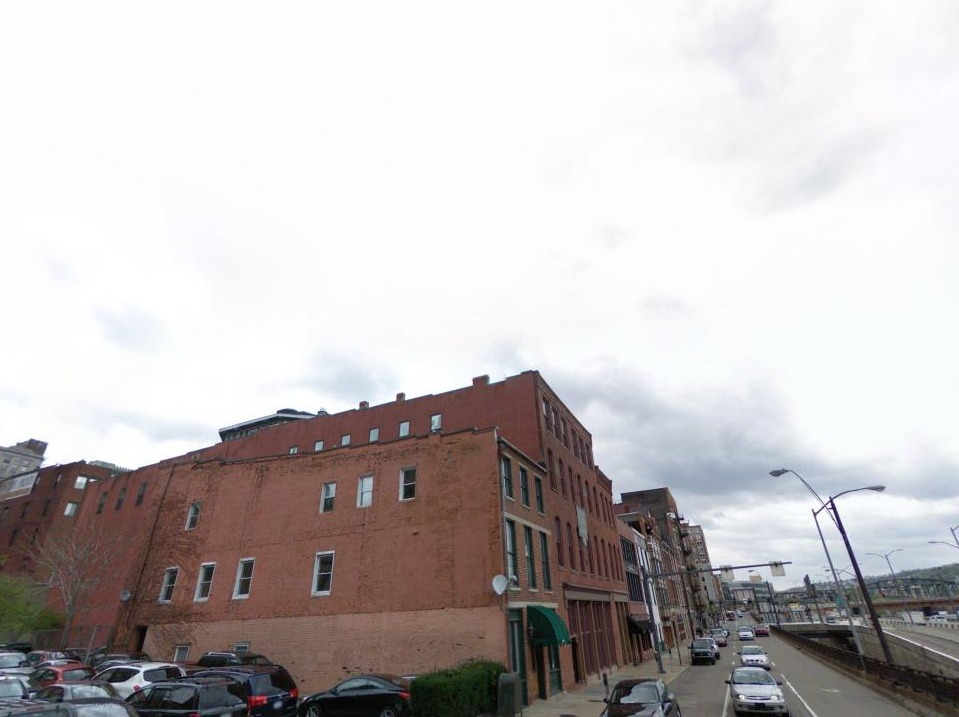
\includegraphics[height=16mm]{imgs/ex4/FV1.jpg}}
        \colorbox{myGreen}{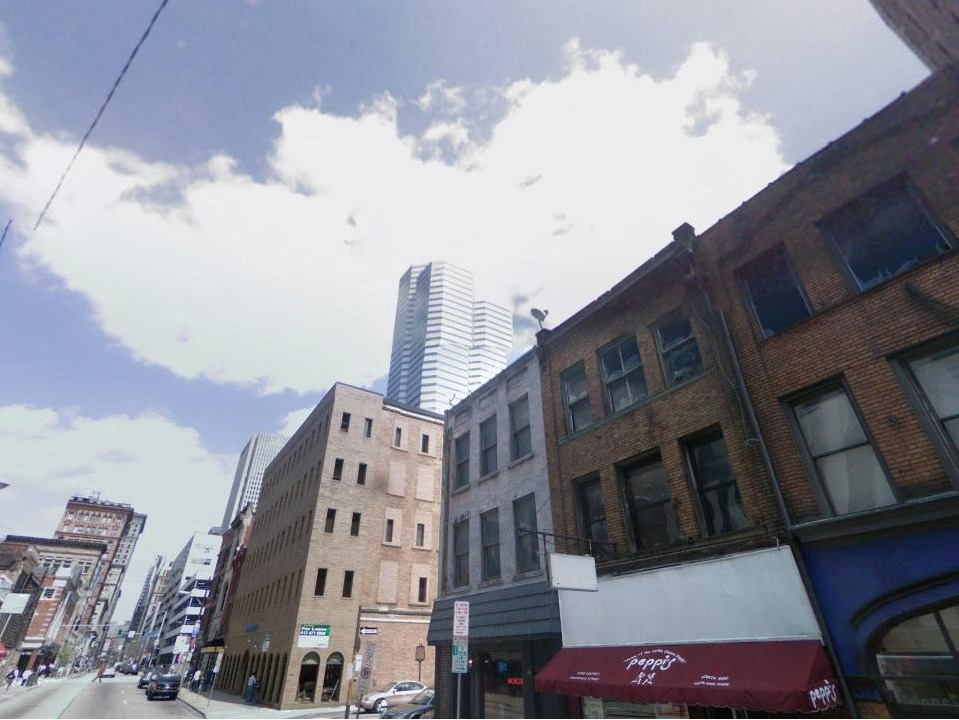
\includegraphics[height=16mm]{imgs/ex4/FV2.jpg}}
        \colorbox{myRed}{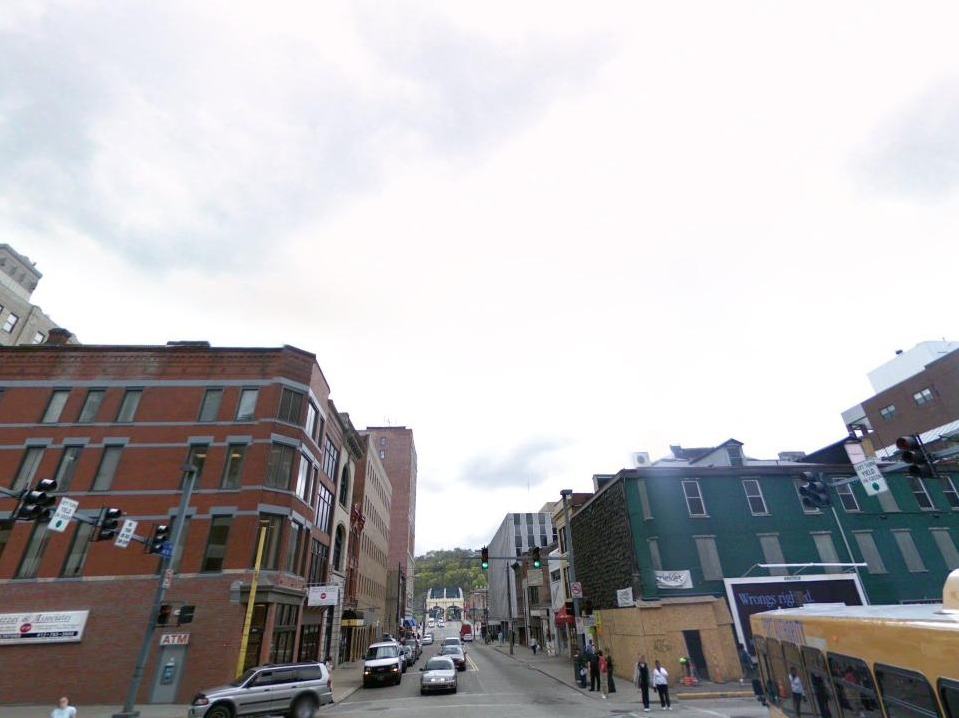
\includegraphics[height=16mm]{imgs/ex4/FV3.jpg}}
        \colorbox{myRed}{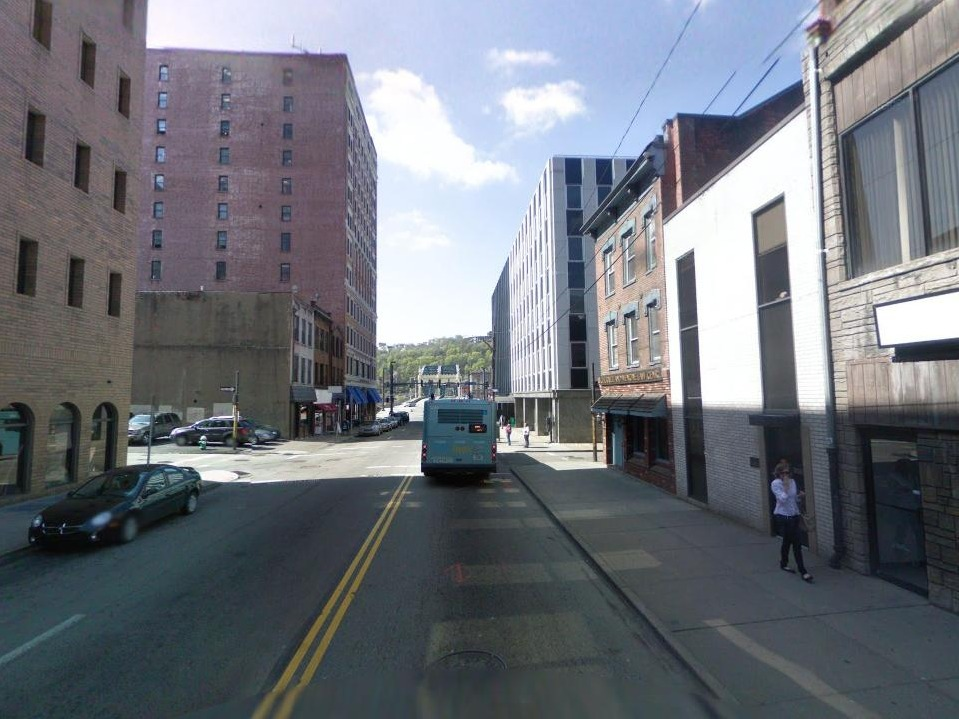
\includegraphics[height=16mm]{imgs/ex4/FV4.jpg}}
    \end{minipage} 
\end{minipage}
%%%%%%%%%%%%%%%%%%%%%%%%%%%%%%%%%%%%%

    In figure~\ref{fig:3qVSw} we visualize the learnt SVM weights on BOW for \emph{p-val}. We visualize the contribution of each feature to the SVM score for the corresponding query image. Red circles represent features with negative weights while green circles correspond to features with positive weights. The area of each circle is proportional to the contribution of the corresponding feature to the SVM score.For instance for the left figure notice that the correctly localized queries (c) contain more green colored features than queries from other places (b) and (a). Query (b) gets a high score because the building has orange and white stripes similar to the the sun-blinds of the bakery, which are features that also have large positive weights in the query image (c) of the correct place.

    In the top row we visualize the calibration of raw SVM score for three different queries. The calibration function of the target image $j$ is shown in the blue and the corresponding SVM scores of the three queries are denoted by red circles. Notice that both images (b) and (c) have high calibrated score even their respective SVM score was different.

    Examples of correctly and incorrectly localized queries are shown in figure \ref{fig:images}. The query image is show in the left column, the shortlist of top four retrieved images is displayed on the right. The first row shows images retrieved by \emph{w-norm} method for FV128 while the second row shows images retrieved by raw Fisher vector.

   % %%%%%%%%%%%%%%%%%%%%%%%%
   % \subsection{Scalability.}
   % %%%%%%%%%%%%%%%%%%%%%%%% 
   %    The linear SVM classifiers trained for each database image are currently non-sparse,
   %    which increases the computational and memory requirements
   %    at query time compared to the original bag-of-visual-words representation.
   %    For a database of 25,000 images, applying all classifiers on a query image takes currently on average 1.72s. The method could be further sped-up by, for example: (i) reducing the dimensionality of the input vectors~\cite{Jegou12}, or (ii) enforcing additional sparsity constraints on learnt weight vectors $w$.


%%%%%%%%%%%%%%%%%%%%%
\section{Conclusions}
%%%%%%%%%%%%%%%%%%%%%
TODO...
Place recognition can be cast as learning \newline
Two calibration methods \newline
Two descriptors \newline
Performance demonstrated on two datasets \newline



\begin{acknowledgements}
   This work was supported by the MSR-INRIA laboratory, the EIT-ICT labs.
   {
   \small
   \noindent
   Supported by the Intelligence Advanced Research Projects Activity (IARPA) via Air Force Research Laboratory. The U.S. Government is authorized to reproduce and distribute reprints for governmental purposes notwithstanding any copyright annotation thereon. Disclaimer:  The views and conclusions contained herein are those of the authors and should not be interpreted as necessarily representing the official policies or endorsements, either expressed or implied, of IARPA, AFRL or the U.S. Government.
   }
\end{acknowledgements}

%%%%%%%%%%%%%%%%%%%%%%%%%%%%%%%%%%%%%%%%%%%%%%%%%%%%%%%%%%%%%%%%%%%%%%%%%%%%
  \begin{figure*}%[tbp]
  \begin{minipage}{0.48\linewidth}
          \begin{minipage}{0.65\linewidth}
            \centering
            {\scriptsize Calibrated classifier score $f_j$}
            \\
            \vspace{2mm}
            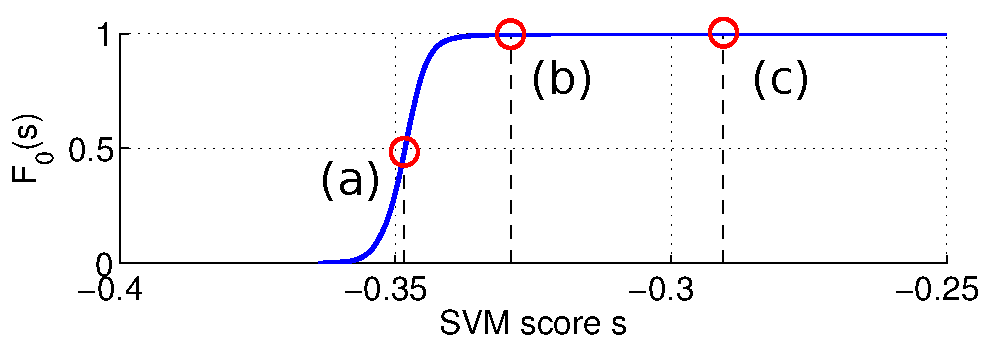
\includegraphics[width=\linewidth]{imgs/wVS3q/2882/graphBigO.pdf}
          \end{minipage} 
          %
          \begin{minipage}{\wii}
            \centering
            \centerline{\scriptsize Target database image $j$}
            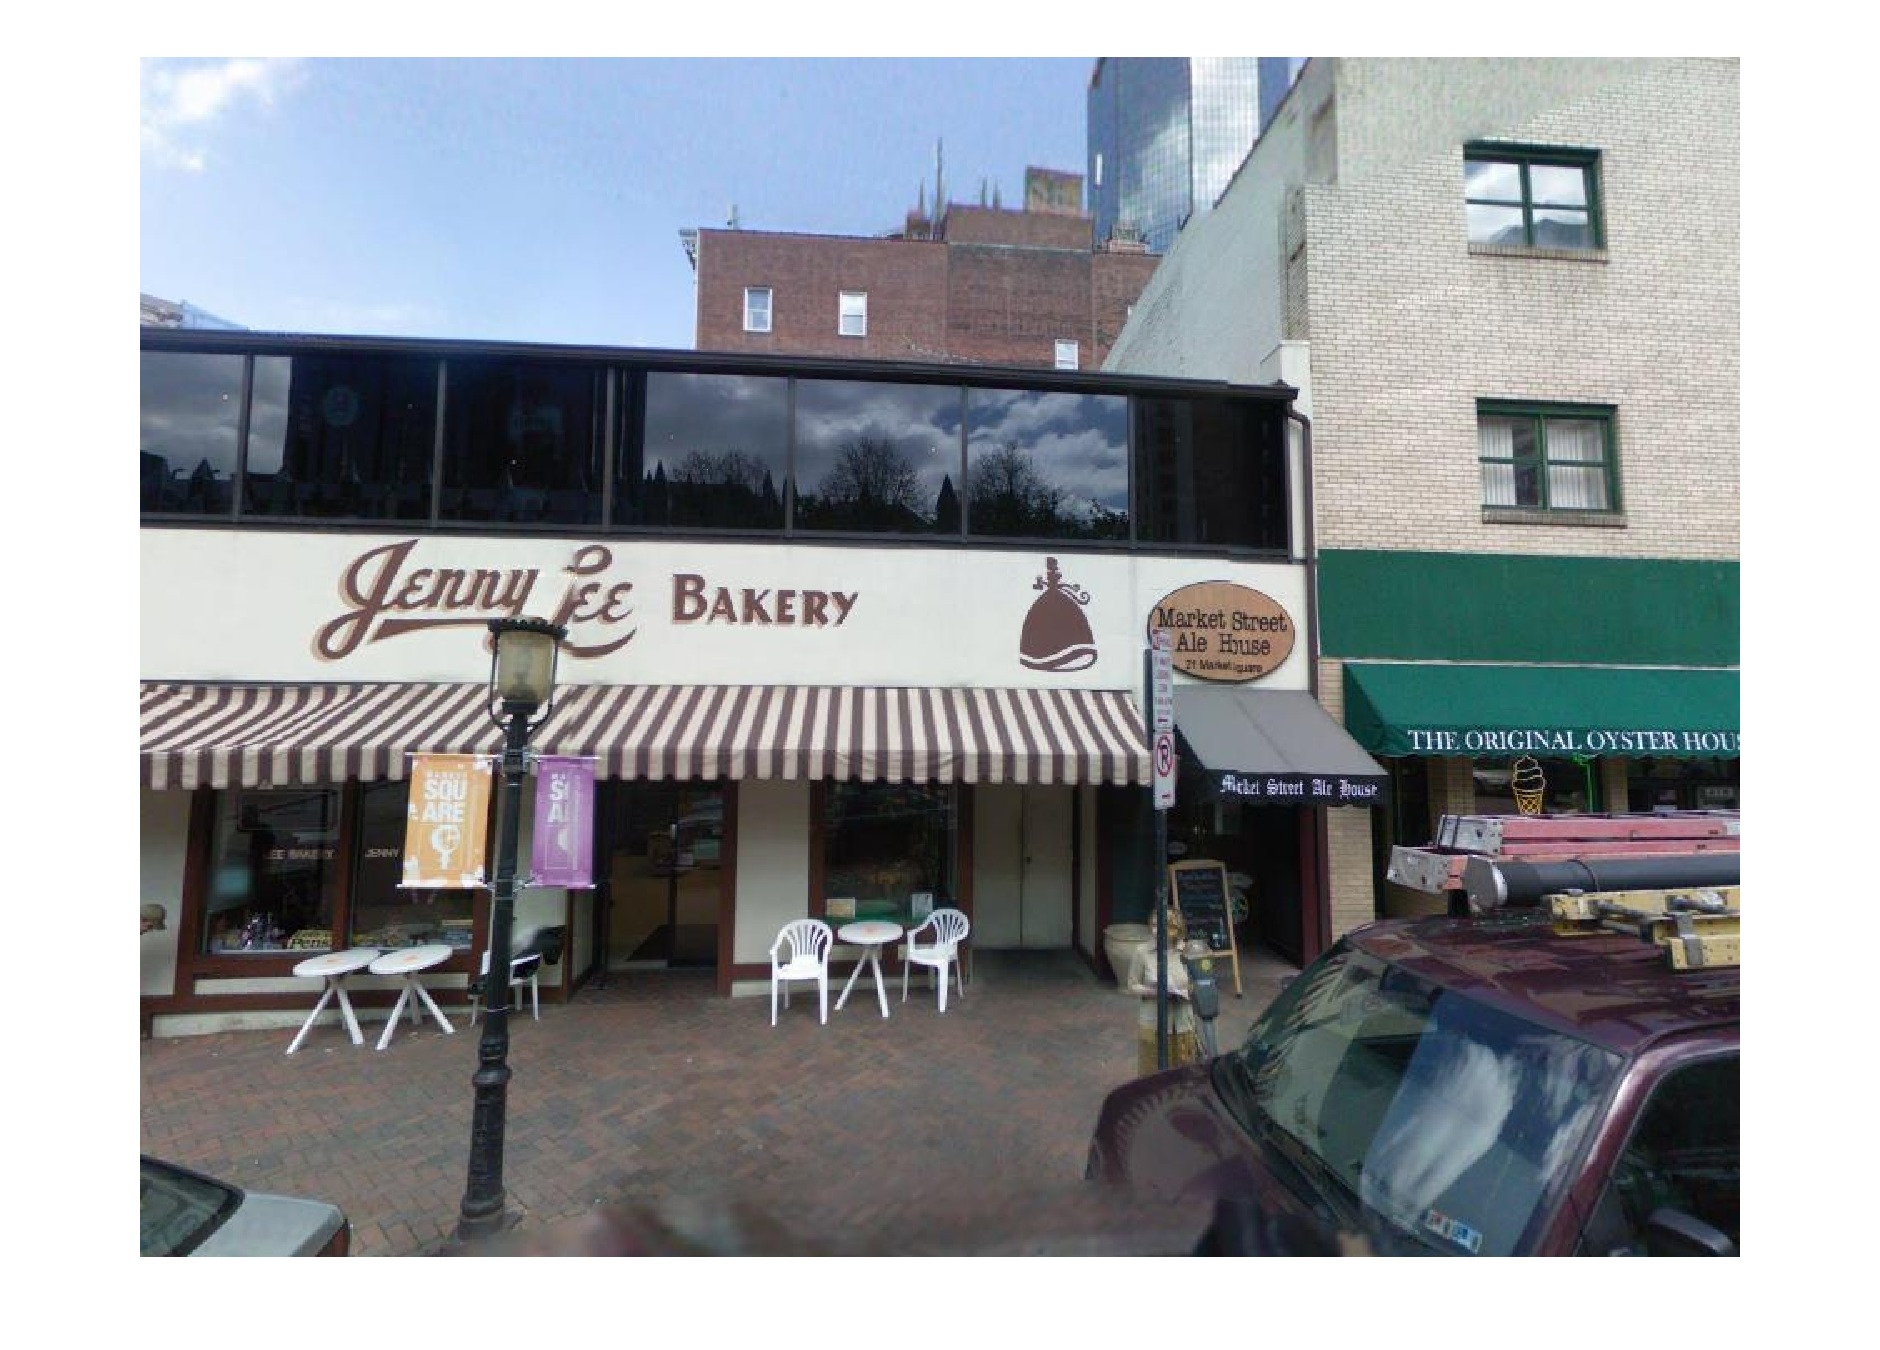
\includegraphics[width=\linewidth]{imgs/wVS3q/2882/j.jpg}
          \end{minipage}  
          \vspace{3mm}
          \\
          \centerline{\scriptsize Classified query images $f_j(q)$} 
          \\
          \begin{minipage}{\wii}
            \centering
            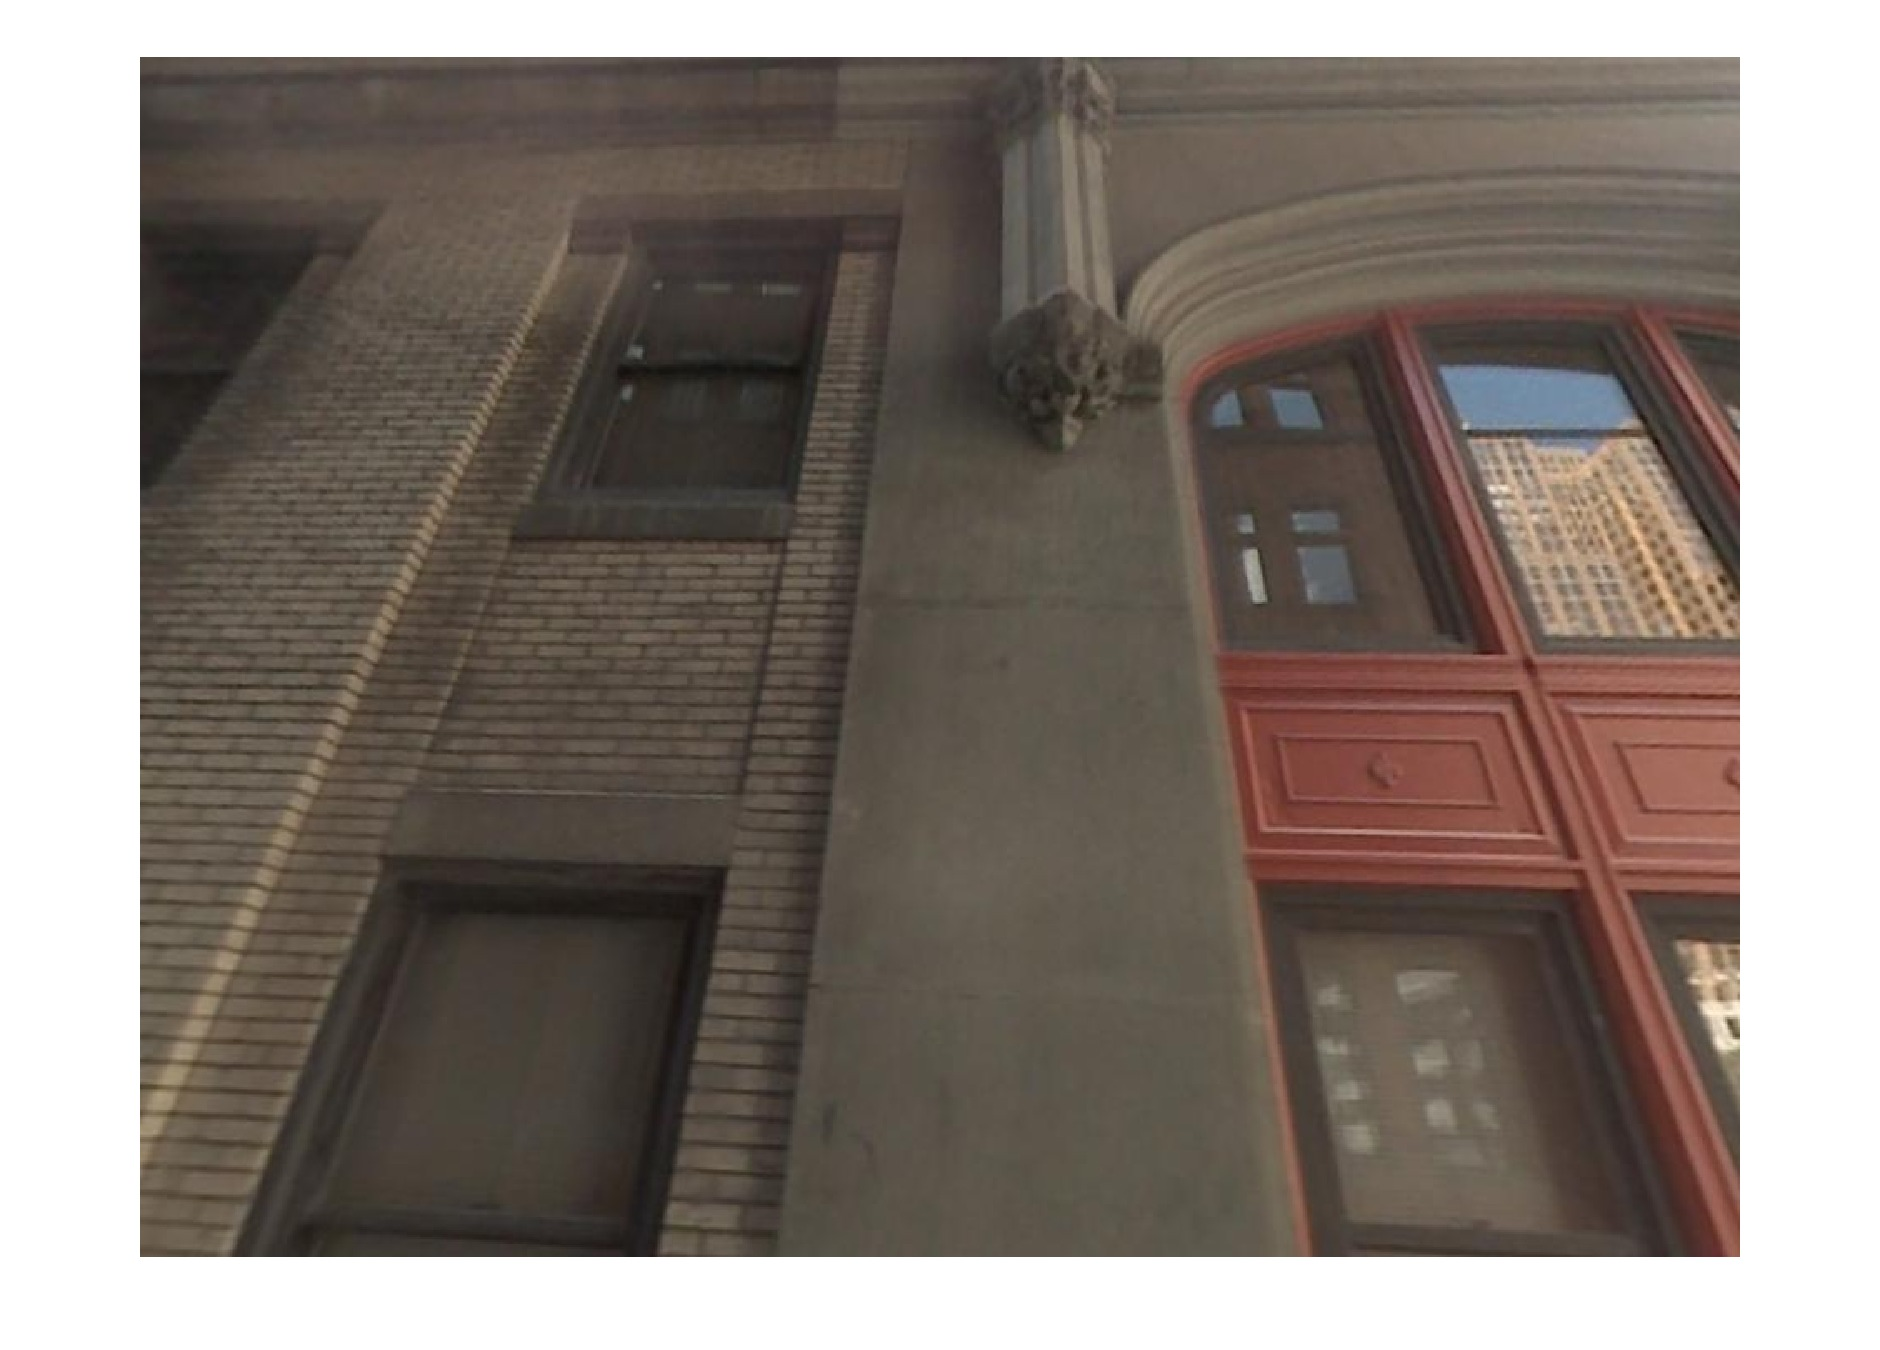
\includegraphics[width=\linewidth]{imgs/wVS3q/2882/a.jpg}
          \end{minipage}
          %  
          \begin{minipage}{\wii}
            \centering
            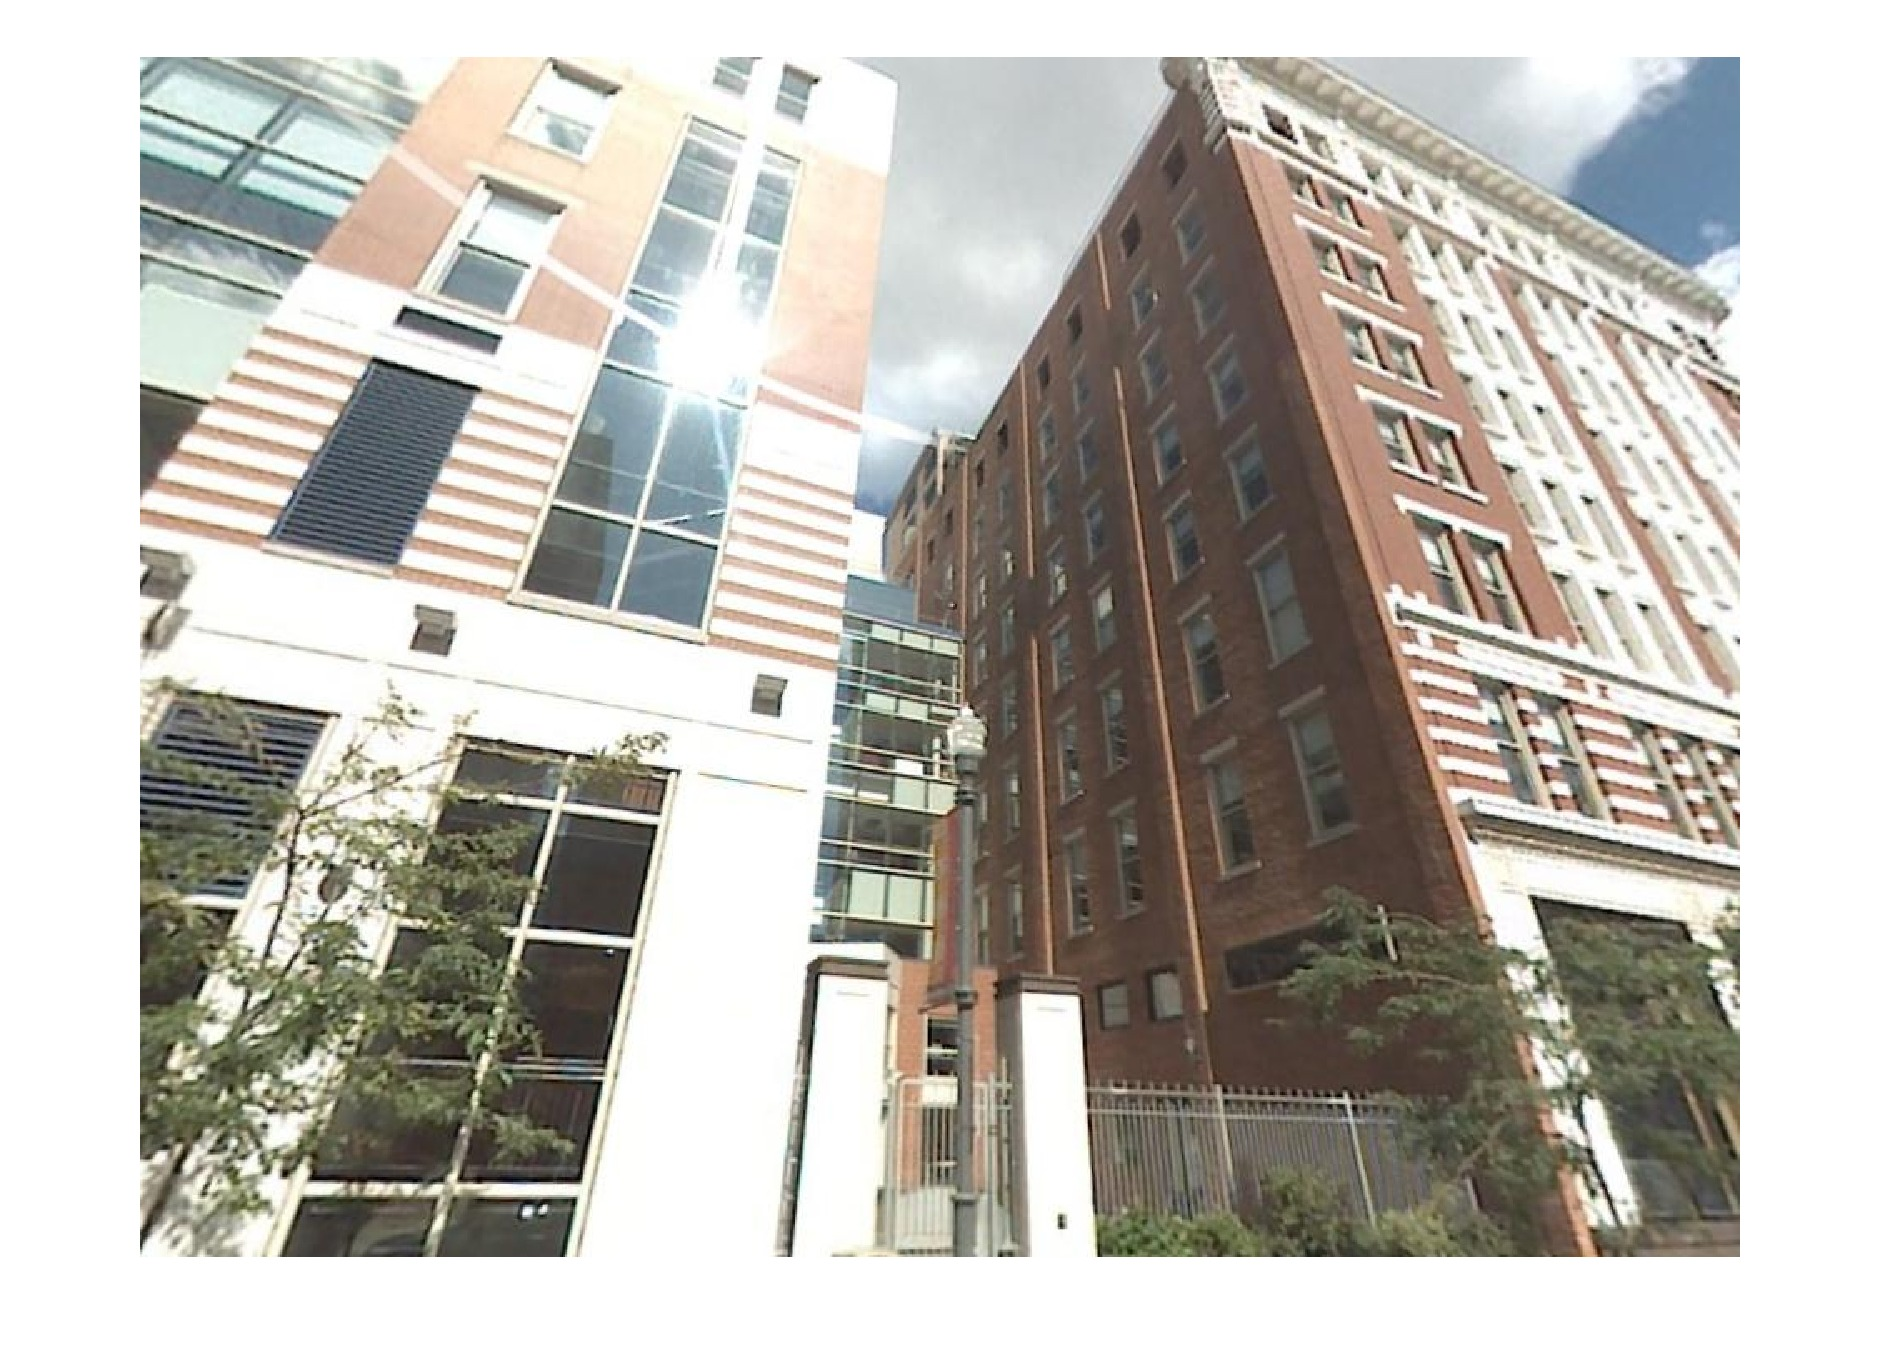
\includegraphics[width=\linewidth]{imgs/wVS3q/2882/b.jpg}
          \end{minipage}
          %  
          \begin{minipage}{\wii}
            \centering
            \includegraphics[width=\linewidth]{imgs/wVS3q/2882/c.jpg}
          \end{minipage} 
          \\
          \begin{minipage}{\wii}
            \centering
            \includegraphics[width=\linewidth]{imgs/wVS3q/2882/aftrs.jpg}
            \newline
            (a)
          \end{minipage}  
          \begin{minipage}{\wii}
            \centering
            \includegraphics[width=\linewidth]{imgs/wVS3q/2882/bftrs.jpg}
            \newline
            (b)
          \end{minipage}  
          \begin{minipage}{\wii}
            \centering
            \includegraphics[width=\linewidth]{imgs/wVS3q/2882/cftrs.jpg}
            \newline
            (c)
          \end{minipage} 
    \end{minipage}% left figure
    %
    %%%%%%%%%%%%%%%%%%%%%%%%%%%%%%%%%
    \begin{minipage}{0.04\linewidth}
      \hspace{\linewidth}
    \end{minipage}
    %%%%%%%%%%%%%%%%%%%%%%%%%%%%%%%%%
    % RIGHT FIGURE
    \begin{minipage}{0.48\linewidth}
          \begin{minipage}{0.66\linewidth}
            \centering
            {\scriptsize Calibrated classifier score $f_j$}
            \\
            \vspace{2mm}
            \includegraphics[width=\linewidth]{imgs/wVS3q/2932/graphBigO.pdf}
          \end{minipage} 
          %
          \begin{minipage}{\wii}
            \centering
            \centerline{\scriptsize Target database image $j$}
            \includegraphics[width=\linewidth]{imgs/wVS3q/2932/j.jpg}
          \end{minipage}  
          \vspace{3mm}
          \\
          \centerline{\scriptsize Classified query images $f_j(q)$} 
          \\
          \begin{minipage}{\wii}
            \centering
            \includegraphics[width=\linewidth]{imgs/wVS3q/2932/a.jpg}
          \end{minipage}  
          \begin{minipage}{\wii}
            \centering
            \includegraphics[width=\linewidth]{imgs/wVS3q/2932/b.jpg}
          \end{minipage}  
          \begin{minipage}{\wii}
            \centering
            \includegraphics[width=\linewidth]{imgs/wVS3q/2932/c.jpg}
          \end{minipage} 
          \\
          \begin{minipage}{\wii}
            \centering
            \includegraphics[width=\linewidth]{imgs/wVS3q/2932/aftrs.jpg}
            \newline
            (a)
          \end{minipage}  
          \begin{minipage}{\wii}
            \centering
            \includegraphics[width=\linewidth]{imgs/wVS3q/2932/bftrs.jpg}
            \newline
            (b)
          \end{minipage}  
          \begin{minipage}{\wii}
            \centering
            \includegraphics[width=\linewidth]{imgs/wVS3q/2932/cftrs.jpg}
            \newline
            (c)
          \end{minipage} 
    \end{minipage}% right figure
    %
    \vspace*{-2mm}
    \caption{\myCap}
    \label{fig:3qVSw}
        \vspace*{2mm}
    \end{figure*}

% BibTeX users please use one of
%\bibliographystyle{spbasic}      % basic style, author-year citations
%\bibliographystyle{spmpsci}      % mathematics and physical sciences
%\bibliographystyle{spphys}       % APS-like style for physics
%\bibliography{}   % name your BibTeX data base

%\bibliographystyle{spbasic}
%\bibliographystyle{spphys}       % APS-like style for physics
\bibliographystyle{spmpsci}      % mathematics and physical sciences

{\footnotesize
\bibliography{shortstrings,vggroup,cvww_template,mybib}
}
%
%% Non-BibTeX users please use
%\begin{thebibliography}{}
%%
%% and use \bibitem to create references. Consult the Instructions
%% for authors for reference list style.
%%
%\bibitem{RefJ}
%% Format for Journal Reference
%Author, Article title, Journal, Volume, page numbers (year)
%% Format for books
%\bibitem{RefB}
%Author, Book title, page numbers. Publisher, place (year)
%% etc
%\end{thebibliography}

\end{document}
% end of file template.tex

